\documentclass[12pt,a4paper]{report}
%\documentclass[12pt,a4paper]{book}
\usepackage[utf8]{inputenc}
\usepackage{fancyhdr}
\usepackage{verbatim}
\usepackage[english]{babel}
\usepackage[superscript,biblabel]{cite}
\usepackage{newlfont}
\usepackage{graphicx}
\usepackage{float}
\usepackage{xpatch}
\usepackage{dirtree}
%\usepackage{listings, xcolor}
\usepackage[hyphenbreaks]{breakurl}
\usepackage[hyphens]{url}
\usepackage{geometry} 
\usepackage[footnotesize,bf]{caption2}
\usepackage{afterpage}
\usepackage{lipsum}
\usepackage{changepage}
\usepackage{caption2}
\usepackage[table]{xcolor}
\usepackage{multirow}
\usepackage{xcolor}
\usepackage{lettrine}
\usepackage{hyperref}
\usepackage{amsbsy}
\usepackage{amsmath}
\usepackage{fancyhdr}
\usepackage{amssymb}
\usepackage{mathtools}
\usepackage{amsthm}
\usepackage{mathrsfs}
\usepackage{mdframed}
\usepackage{tocloft}
\usepackage[most]{tcolorbox}%se hai problemi con immagini, rimuovi most e rivedi fillfigure
\usepackage{pgfplots}
\usepackage{eso-pic}
\usepackage{tikz}
\usepackage{physics}
\usepackage{blkarray, bigstrut} %
\usepackage[explicit]{titlesec}


%%%%%%%%%%%%%%%%%%%%%%%%%%%%%%%%%%%%%%%%%%%%%%%%%%%%%%%%
%%%%%%%%%%%%%%%%%%%%%%%%% MISC %%%%%%%%%%%%%%%%%%%%%%%%%
%%%%%%%%%%%%%%%%%%%%%%%%%%%%%%%%%%%%%%%%%%%%%%%%%%%%%%%%

\setcounter{tocdepth}{4}
\tcbuselibrary{theorems}
\textwidth=5000pt\oddsidemargin=0pt
\geometry{top=20mm, bottom=20mm, left=20mm, right=20mm}
\renewcommand{\baselinestretch}{1.1}
\renewcommand{\chaptermark}[1]{%
  \markboth{#1}{}}
\makeatletter \renewcommand{\@citess}[1]{\textsuperscript{\,[#1]}} \makeatother

\hypersetup{
  urlcolor=green!70!black
}
%%%%%%%%%%%%%%%%%%%%%%%%%%%%%%%%%%%%%%%%%%%%%%%%%%%%%%%%%%%%%%%%
%%%%%%%%%%%%%%%%%%%%%%%%% FAST PICTURE %%%%%%%%%%%%%%%%%%%%%%%%%
%%%%%%%%%%%%%%%%%%%%%%%%%%%   and   %%%%%%%%%%%%%%%%%%%%%%%%%%%% 
%%%%%%%%%%%%%%%%%% FAST FILLHEIGHT PICTURE PICTURE  %%%%%%%%%%%%
%%%%%%%%%%%%%%%%%%%%%%%%%%%%%%%%%%%%%%%%%%%%%%%%%%%%%%%%%%%%%%%%

\newcommand{\fastpic}[3]{
\begin{figure}[H]
                \centering
                        \includegraphics[width=#3\textwidth]{#1}
 \caption{#2} 
\end{figure}
}

\newcommand\remheight{\dimexpr\pagegoal-\pagetotal-\baselineskip\relax}
\newtcolorbox{fillfigure}[1][]{height fill, space to=\myspace,#1}

\newcommand{\fastfpic}[2]{
\begin{fillfigure}[blanker]
            \centering 
            \includegraphics[ height=\myspace]{#1}\\
            \captionof{figure}{#2}
            \end{fillfigure}
}

%%%%%%%%%%%%%%%%%%%%%%%%%%%%%%%%%%%%%%%%%%%%%%%%%%%%%%%%
%%%%%%%%%%%%%%%%%%%% OTHER FAST COMMANDS %%%%%%%%%%%%%%%
%%%%%%%%%%%%%%%%%%%%%%%%%%%%%%%%%%%%%%%%%%%%%%%%%%%%%%%%

%%FAST RNNLCOMB, IN CHAPTER 5 RNN, (JUST A COMPACT NOTATION)
\newcommand{\rnnlcomb}[1]{\left( \ov{W}_{#1}\ov{x}_t+\ov{U}_{#1}\ov{h}_{t-1}+\ov{V}_{#1}\ov{c}_{t-1} +\ov{b}_{#1} \right)}

%FAST OVERLINE
\newcommand{\ov}[1]{\overline{#1}}

%math things
\newcommand{\bs}[1]{\boldsymbol{#1}}
\newcommand{\R}{\mathbb{R}}
\newcommand{\Z}{\mathbb{Z}}
\newcommand{\T}{\mathbb{T}}
\newcommand{\I}{\mathbb{I}}
\newcommand{\N}{\mathbb{N}}
\newcommand{\E}{\mathbb{E}}
\newcommand{\A}{\mathbb{A}}
\newcommand{\bfE}{\mathbf{E}}
\newcommand{\bfP}{\mathbf{P}}
\newcommand{\red}[1]{\textcolor{red}{#1}}
\newcommand{\blue}[1]{\textcolor{blue}{#1}}
\newcommand{\Lagr}{\mathcal{L}}
\newcommand{\Sm}{\mathbb{S}^{(m)}}
\newcommand{\nrm}[1]{\left\Vert{#1}\right\Vert}
\NewDocumentCommand{\evalat}{sO{\big}mm}{%
  \IfBooleanTF{#1}
   {\mleft. #3 \mright|_{#4}}
   {#3#2|_{#4}}%
}

\DeclarePairedDelimiter\floor{\lfloor}{\rfloor}
\DeclarePairedDelimiter\ceil{\lceil}{\rceil}

%Partial derivate shortcommand
\newcommand{\deinde}[2]{\frac{\partial #1}{\partial #2}}

%centered italic highlighted text, with/without rules
\newcommand{\hhhRule}[1]{
 \begin{adjustwidth}{25mm}{25mm}
                 \rule[0.1cm]{12cm}{0.6mm}\\
                 \centering
                    \textit{#1}\\
        \rule[0.1cm]{12cm}{0.6mm}\\
\end{adjustwidth}
}
\newcommand{\hhhNoRule}[1]{
 \begin{adjustwidth}{25mm}{25mm}
                 \centering
                    \textit{#1}\\
\end{adjustwidth}
}

%For circled numbers, require tikz
\newcommand*\circled[1]{\tikz[baseline=(char.base)]{
            \node[shape=circle,draw,inner sep=2pt] (char) {#1};}}
            
\title{More than one Author with different Affiliations}
\author{Lorenzo Epifani}



%for equation emum
\newcommand{\myequation}{\begin{equation}}
\newcommand{\myendequation}{\end{equation}}
\let\[\myequation
\let\]\myendequation


%bg equation env
\newtcolorbox{eqbox}[1][]
{
colback=gray!10,
arc=0pt,
boxrule=-1pt,
title=#1 % I would like to make this (one of these in general) assignment optional depending on #1, #2...
}

 \newenvironment{eqwbg}[1][]{
    \begin{eqbox}[#1]
    \[
 }{
   \]
   \end{eqbox}\vspace{-17pt} \phantom{a}\\\noindent} %MACRO, COMANDI E CONFIG VARIE

\begin{document}
\newcommand{\pyin}[1]{\colorbox{light-gray}{{\texttt{\lstinline[language=Python]{#1}}}}}
\definecolor{light-gray}{gray}{0.95}
\definecolor{COMMENT}{HTML}{339966}
\definecolor{KEY1}{HTML}{993399}
\definecolor{NUM}{HTML}{ccff33}
\definecolor{STRING}{HTML}{cc6600}
\definecolor{KEY2}{HTML}{0000FF}
\definecolor{KEY3}{HTML}{0066ff}

\lstset{
  backgroundcolor=\color{light-gray},  % choose the background color
  basicstyle=\footnotesize,
  breaklines=true,                % automatic line breaking only at whitespace
  escapeinside={\%*}{*)},         % if you want to add LaTeX within your code
}

\lstdefinelanguage{Python}{
columns=fullflexible,  %Delete this line if you don t want to copy/paste code from pdf
showstringspaces=false,
morestring=[b]",
morestring=[b]',
morecomment=[l]{\#},
commentstyle=\color{COMMENT},   
numberstyle=\tiny\color{NUM},
stringstyle=\color{STRING},
basicstyle=\ttfamily\footnotesize,
breakatwhitespace=false,
classoffset=1,
    morekeywords={False,None,True},
    keywordstyle=\color{KEY2}\bfseries,
classoffset=2,
    morekeywords={and,as,assert,break,class,continue,def,del,elif,else,except,finally,for,from,global,if,import,in,is,lambda,nonlocal,not,or,pass,raise,return,try,while,with,yield,this},
    keywordstyle=\color{KEY1}\bfseries,
classoffset=3,
    morekeywords={ArithmeticError, AssertionError, AttributeError, BaseException, BlockingIOError, BrokenPipeError, BufferError, BytesWarning, ChildProcessError, ConnectionAbortedError, ConnectionError, ConnectionRefusedError, ConnectionResetError, DeprecationWarning, EOFError, Ellipsis, EnvironmentError, Exception, False, FileExistsError, FileNotFoundError, FloatingPointError, FutureWarning, GeneratorExit, IOError, ImportError, ImportWarning, IndentationError, IndexError, InterruptedError, IsADirectoryError, KeyError, KeyboardInterrupt, LookupError, MemoryError, ModuleNotFoundError, NameError, None, NotADirectoryError, NotImplemented, NotImplementedError, OSError, OverflowError, PendingDeprecationWarning, PermissionError, ProcessLookupError, RecursionError, ReferenceError, ResourceWarning, RuntimeError, RuntimeWarning, StopAsyncIteration, StopIteration, SyntaxError, SyntaxWarning, SystemError, SystemExit, TabError, TimeoutError, True, TypeError, UnboundLocalError, UnicodeDecodeError, UnicodeEncodeError, UnicodeError, UnicodeTranslateError, UnicodeWarning, UserWarning, ValueError, Warning, ZeroDivisionError, _, __build_class__, __debug__, __doc__, __import__, __loader__, __name__, __package__, __spec__, abs, all, any, ascii, bin, bool, bytearray, bytes, callable, chr, classmethod, compile, complex, copyright, credits, delattr, dict, dir, divmod, enumerate, eval, exec, exit,filter, float, format, frozenset, getattr, globals, hasattr, hash, help, hex, id, input, int, isinstance, issubclass, iter, len, license, list, locals, map, max, memoryview, min, next, object, oct, open, ord, pow, print, property, quit, range, repr, reversed, round, set, setattr, slice, sorted, staticmethod, str, sum, super, tuple, type, vars, zip},
    keywordstyle=\color{KEY3}\bfseries,
}




 %PYTHON STYLE LANG
\definecolor{FRM}{HTML}{337BA1}
\definecolor{BGF}{HTML}{EDF1F2}
\definecolor{BRD}{HTML}{343742}

\newcommand{\boxA}[1]{
\begin{tcolorbox}[enhanced,sharp corners=uphill,
    width=10cm,
    colback=BGF,
    colframe=FRM,
    coltext=black,
    fontupper=\Large\bfseries,
    arc=6mm,
    boxrule=8pt,
    boxsep=2mm,
    borderline={2pt}{8pt}{BRD}]
    \centering
\textbf{#1} \\
\textbf{notes}
\end{tcolorbox}
}

\newcommand{\boxB}[1]{
\begin{tcolorbox}[enhanced jigsaw,
                  colback=bgframe,%gray background
                  colframe=frame,% black frame colour
                  width=6cm,% Use 5cm total width,
                  arc=3mm, auto outer arc,
                  boxrule=3pt,
                  drop shadow={frame!80}
                 ]
                 \centering
\textbf{#1} \\
\textbf{notes}
\end{tcolorbox}
}





\begin{titlepage}
\begin{picture}(50,50)
%\put(-15,-185){\hbox{\includegraphics[scale=0.30]{pics/fronts/unisalento.png}}}
\end{picture}
%\includegraphics[viewport= -3400 1500 0 0, scale=0.12]{pics/NODE.png}

%width=\paperwidth
%height=\paperheight

\AddToShipoutPictureBG*{\includegraphics[width=\paperwidth]{pics/fronts/bg3.jpg}}

%\includegraphics[viewport= -100 470 0 0, scale=1]{pics/brainLogo.png}
\begin{center}
\scalebox{1.5}{
\boxA{Applied Data Science}
      }
\end{center}
\vspace{140mm}
\begin{large}
    \begin{flushleft}
    \end{flushleft}
\end{large}
\end{titlepage}  %FRONTESPIZIO
\noindent \textbf{Author}:\phantom{xxxix} Lorenzo Epifani\\
\textbf{Email}:\phantom{xxxxxx} lorenzo.epifani1@studenti.unisalento.it
\\\vspace{50px}\phantom{a}\\
\noindent These notes have been written with the  purpose of synthesizing in a single document the different topics dealt with in the second-level master's degree course "\href{https://www.dii.unisalento.it/master/applied-data-science}{\textbf{Applied Data Science}} - \textbf{University of Salento}". 
This document is the result of the integration between the transcription of the content of the didactic courses and the material (mainly books and academic papers) indicated in the "Bibliography" section.
\pagebreak %PREAMBOLO
%%%%%%%%%%%%%%%%%%%%%%%%%%%%%%%%%%%%%%%%%%%%%%%%%%%%%%%%%%%%%%%%
%%%%%%%%%%%%%%%%%%%%%%%%% CHAPTER STYLE %%%%%%%%%%%%%%%%%%%%%%%%
%%%%%%%%%%%%%%%%%%%%%%%%%%%%%%%%%%%%%%%%%%%%%%%%%%%%%%%%%%%%%%%%

%NUMBERED CHA
\titleformat{\chapter}[display]
  {\normalfont\huge\bfseries}
  {}
  {20pt}
  {%
    \begin{tcolorbox}[
      borderline north = {0.65mm}{3.2mm}{black},
      borderline south = {0.65mm}{3.2mm}{black},
      enhanced,
      colback=BGF,
      boxrule=0.25cm,
      colframe=FRM,
      arc=0pt,
      outer arc=0pt,
      leftrule=0pt,
      rightrule=0pt,
      fontupper=\color{black}\sffamily\bfseries\huge,
      enlarge left by=-1in-\hoffset-\oddsidemargin, 
      enlarge right by=-\paperwidth+1in+\hoffset+\oddsidemargin+\textwidth,
      width=\paperwidth, 
      left=1cm+\hoffset+\oddsidemargin, 
      right=\paperwidth-1in-\hoffset-\oddsidemargin-\textwidth,
      top=0.9cm, 
      bottom=0.15cm,
      overlay={
        \node[
          circle, 
          fill=BGF,
          draw=FRM,
          line width=0.20cm,
          inner sep=0pt,
          text width=2cm,
          minimum height=2cm,
          align=center,
          font=\color{black}\sffamily\bfseries\fontsize{30}{36}\selectfont
        ] 
        (chapname)
        at ([xshift=-4cm]frame.north east)
        {\huge \scalebox{1.7}{\thechapter}};
        \node[font=\small,anchor=south,inner sep=2pt] at (chapname.north)
        {\scalebox{1.5}{\MakeUppercase\chaptertitlename}};  % if using amsbook, this should be \chaptername
      } 
    ]
    \scalebox{1}{#1}
    \end{tcolorbox}%
    \vspace{-2.5cm}
  }


%%%% UNNUMBERED  CHA
\titleformat{name=\chapter,numberless}[display]
  {\normalfont\huge\bfseries}
  {}
  {20pt}
  {%
    \begin{tcolorbox}[
      borderline north = {0.65mm}{3.2mm}{black},
      borderline south = {0.65mm}{3.2mm}{black},
      enhanced,
      colback=BGF,
      boxrule=0.25cm,
      colframe=FRM,
      arc=0pt,
      outer arc=0pt,
      leftrule=0pt,
      rightrule=0pt,
      fontupper=\color{black}\sffamily\bfseries\huge,
      enlarge left by=-1in-\hoffset-\oddsidemargin, 
      enlarge right by=-\paperwidth+1in+\hoffset+\oddsidemargin+\textwidth,
      width=\paperwidth, 
      left=1cm+\hoffset+\oddsidemargin, 
      right=\paperwidth-1in-\hoffset-\oddsidemargin-\textwidth,
      top=0.9cm, 
      bottom=0.15cm,
    ]
    \scalebox{1}{#1}
    \end{tcolorbox}%
    \vspace{-2.5cm}
  }
%%%%%%%%%%%%%%%%%%%%%%%%%%%%%%%%%%%%%%%%%%%%%%%%%%%%%%%%%%%%%%%%
%%%%%%%%%%%%%%%%%%%%%%%%% SECTION STYLE %%%%%%%%%%%%%%%%%%%%%%%%
%%%%%%%%%%%%%%%%%%%%%%%%%%%%%%%%%%%%%%%%%%%%%%%%%%%%%%%%%%%%%%%%  

%NUMBERED SEC
\titleformat{\section}[display]
  {\normalfont\large\bfseries}
  {}
  {20pt}
  {%
    \begin{tcolorbox}[
      enhanced,
      hbox,
      colback=FRM,
      boxrule=0.07cm,
      colframe=black,
      arc=0pt,
      outer arc=0pt,
      leftrule=0pt,
      rightrule=0.07cm,
      fontupper=\color{black}\sffamily\bfseries\Large,
      enlarge left by=-1in-\hoffset-\oddsidemargin, 
      enlarge right by=-\paperwidth+1in+\hoffset+\oddsidemargin+\textwidth,
      width=\textwidth, 
      left=0.4in+\hoffset+\oddsidemargin, 
      right=\paperwidth-1in-\hoffset-\oddsidemargin-\textwidth,
      top=0.5cm, 
      bottom=0.1cm,
      overlay={
        \node[
          fill=BGF ,
          draw=FRM,
          line width=0.07cm,
          inner sep=0pt,
          text width=5cm,
          minimum height=0.8cm,
          align=center,
          font=\color{black}\sffamily\bfseries\fontsize{30}{36}\selectfont
        ] 
        (chapname)
        at ([xshift=+3cm, yshift=+4pt ]frame.north west)
        {\Large Section: \thesection};
        \node[font=\small,anchor=south,inner sep=2pt] at (chapname.north)
        {};  % if using amsbook, this should be \chaptername
               \draw[line width=8pt, BGF] (0,-0.06) -- (0.8\paperwidth,-0.06);
      } 
    ]
    \scalebox{1.1}{\textcolor{white}{#1}}
    \end{tcolorbox}%
    \vspace{-1cm}
  }
  
% UNNUMBERED SEC
\titleformat{name=\section, numberless}[display]
  {\normalfont\large\bfseries}
  {}
  {20pt}
  {%
    \begin{tcolorbox}[
      enhanced,
      hbox,
      colback=FRM,
      boxrule=0.07cm,
      colframe=black,
      arc=0pt,
      outer arc=0pt,
      leftrule=0pt,
      rightrule=0.07cm,
      fontupper=\color{black}\sffamily\bfseries\Large,
      enlarge left by=-1in-\hoffset-\oddsidemargin, 
      enlarge right by=-\paperwidth+1in+\hoffset+\oddsidemargin+\textwidth,
      width=\textwidth, 
      left=0.4in+\hoffset+\oddsidemargin, 
      right=\paperwidth-1in-\hoffset-\oddsidemargin-\textwidth,
      top=0.5cm, 
      bottom=0.1cm,
      overlay={
      \node[
          anchor=south,
          fill=BGF,
          line width=0pt,
          inner sep=0pt,
          text width=\paperwidth,
          right=2cm,
          minimum height=0.9mm,
          align=center,
        ] 
        (aa)
        at ([xshift=-2cm,yshift=-1.5cm]frame.north west)
        {};
        \draw[line width=8pt, BGF] (0,-0.06) -- (0.8\paperwidth,-0.06);}
    ]
    \scalebox{1.1}{\textcolor{white}{#1}}
    \end{tcolorbox}%
    \vspace{-1cm}
  }
%%%%%%%%%%%%%%%%%%%%%%%%%%%%%%%%%%%%%%%%%%%%%%%%%%%%%%%%%%%%%%%%
%%%%%%%%%%%%%%%%%%%%%%%%% SUBSECTION STYLE %%%%%%%%%%%%%%%%%%%%%%%%
%%%%%%%%%%%%%%%%%%%%%%%%%%%%%%%%%%%%%%%%%%%%%%%%%%%%%%%%%%%%%%%%

%NUMBERED SUB
\titleformat{\subsection}[display]
  {\normalfont\large\bfseries}
  {}
  {20pt}
  {%
    \begin{tcolorbox}[
      enhanced,
      hbox,
      colback=BGF,
      boxrule=0pt,
      colframe=FRM,
      arc=0pt,
      outer arc=0pt,
      leftrule=0pt,
      rightrule=0pt,
      fontupper=\color{black}\sffamily\bfseries\Large,
      width=\textwidth-3cm, 
      left=0.3in,
      enlarge left by=-1in-\hoffset-\oddsidemargin, 
      right=\paperwidth-1in-\hoffset-\oddsidemargin-\textwidth,
      top=0.1cm, 
      bottom=0.1cm,
      overlay={
        \node[
          fill=FRM,
          line width=0pt,
          inner sep=0pt,
          text width=5cm,
          minimum height=0.8cm,
          align=center,
          font=\color{black}\sffamily\bfseries\fontsize{30}{36}\selectfont
        ] 
        (chapname)
        at ([xshift=+1.8cm, yshift=+12pt]frame.north west)
        {\small  \textcolor{white}{Subsection \thesubsection:} };
        \node[font=\small,anchor=south,inner sep=2pt] at (chapname.north)
        {};  % if using amsbook, this should be \chaptername
      } 
    ]
    \scalebox{0.9}{#1}
    \end{tcolorbox}%
    \vspace{-0.8cm}
  }
  
%UNNUMBERED SUB
\titleformat{name=\subsection,numberless}[display]
  {\normalfont\large\bfseries}
  {}
  {20pt}
  {%
    \begin{tcolorbox}[
      enhanced,
      hbox,
      colback=BGF,
      boxrule=0pt,
      colframe=FRM,
      arc=0pt,
      outer arc=0pt,
      leftrule=0pt,
      rightrule=0pt,
      fontupper=\color{black}\sffamily\bfseries\Large,
      width=\textwidth-3cm, 
      left=0.3in,
      enlarge left by=-1in-\hoffset-\oddsidemargin, 
      right=\paperwidth-1in-\hoffset-\oddsidemargin-\textwidth,
      top=0.1cm, 
      bottom=0.1cm,
    ]
    \scalebox{0.9}{#1}
    \end{tcolorbox}%
    \vspace{-0.8cm}
  }
%%%%%%%%%%%%%%%%%%%%%%%%%%%%%%%%%%%%%%%%%%%%%%%%%%%%%%%%
%%%%%%%%%%%%%%%%%%% HEADER AND FOOTER %%%%%%%%%%%%%%%%%%
%%%%%%%%%%%%%%%%%%%%%%%%%%%%%%%%%%%%%%%%%%%%%%%%%%%%%%%%

\fancypagestyle{myheader}{%
  \fancyhf{}% Clear all headers/footers
  \fancyhead[R]{%
  \begin{tcolorbox}[enhanced,hbox,
  arc=0pt,
  outer arc=0pt,
  left=2pt,
  right=2pt,
  top=2pt,
  bottom=2pt,
  leftrule=0pt,
  bottomrule=1.5pt,
  rightrule=1.5pt,
  toprule=1.5pt,
  colback=BGF,colframe=FRM]
  \hfill \leftmark
\end{tcolorbox}\vspace{-32pt}}% Header Centred
  \fancyfoot[C]{\thepage}% Footer Centred
  %\fancyfoot[L]{\rightmark}
  
  \renewcommand{\headrulewidth}{1.5pt}% 2pt header rule
  \renewcommand{\headrule}{\hbox to\headwidth{%
    \color{FRM}\leaders\hrule height \headrulewidth\hfill}}
    
  \renewcommand{\footrulewidth}{2pt}% No footer rule
  \renewcommand{\footrule}{\hbox to\headwidth{%
    \color{FRM}\leaders\hrule height \footrulewidth\hfill}}
}
\setlength{\headheight}{21pt}%
\pagestyle{myheader}

%%%%%%%%%%%%%%%%%%%%%%%%%%%%%%%%%%%%%%%%%%%%%%%%%%%%%%%%
%%%%%%%DEFINITIONS/PROPERTIES/THEOREMS  STYLE  %%%%%%%%%
%%%%%%%%%%%%%%%%%%%%%%%%%%%%%%%%%%%%%%%%%%%%%%%%%%%%%%%%

\theoremstyle{definition}

%customdef
\newmdtheoremenv[linewidth=2.0pt,%
backgroundcolor=gray!8!blue!5,
innertopmargin=0pt,
linecolor=blue!40,%
roundcorner=5pt,%
]
{customDef}{\colorbox{blue!40}{Definition}}[chapter]

%customProp
\newmdtheoremenv[linewidth=2.0pt,%
backgroundcolor=gray!8!red!5,
innertopmargin=0pt,
linecolor=red!40,%
roundcorner=5pt,%
]{customProp}{\colorbox{red!40}{Property}}[chapter]

%customTheo
\newmdtheoremenv[linewidth=2.0pt,%
backgroundcolor=gray!8!green!5,
innertopmargin=0pt,
linecolor=green!40,%
roundcorner=5pt,%
]{customTheo}{\colorbox{green!40}{Theorem}}[chapter]

%%%%%%%%%%%%%%%%%%%%%%%%%%%%%%%%%%%%%%%%%%%%%%%%%%%%%%%%%%%%%%%%
%%%%%%%%%%%%%%%%%%%%%%%%% TOC STYLE %%%%%%%%%%%%%%%%%%%%%%%%
%%%%%%%%%%%%%%%%%%%%%%%%%%%%%%%%%%%%%%%%%%%%%%%%%%%%%%%%%%%%%%%% 
\makeatletter
\renewcommand\tableofcontents{%
  \null 
  \begin{tcolorbox}[enhanced,hbox,sharp corners=uphill,
    coltext=black,
    colback=BGF,
    fontupper=\Large\bfseries,arc=6mm,boxrule=2.5mm,boxsep=5mm,
    colframe=FRM,
    right=3cm,
    borderline={0.6mm}{0mm}{black},
    overlay={
        \node[
          fill=FRM,
          line width=0pt,
          inner sep=0pt,
          text width=11cm,
          right=2cm,
          minimum height=1.3mm,
          align=center,
        ] 
        (chapname)
        at ([xshift=7.17cm, yshift=-1.2cm]frame.north west)
        {};
        \node[
          fill=FRM,
          line width=0pt,
          inner sep=0pt,
          text width=8cm,
          right=2cm,
          minimum height=1.3mm,
          align=center,
        ] 
        (chapname)
        at ([xshift=-10cm, yshift=-1.2cm]frame.north west)
        {};
      } 
    ]
 \scalebox{1.6}{\contentsname}
\end{tcolorbox}
  \hfill\null\par
  \@mkboth{\MakeUppercase\contentsname}{\MakeUppercase\contentsname}%
  \@starttoc{toc}%
}

%TOC CONTENT STYLE
\xpatchcmd\l@chapter{#1}{\colorbox{FRM}{\textcolor{white}{#1}}}{}{}

\xpatchcmd\l@section{#1}{\colorbox{BGF}{\textcolor{black}{#1}}}{}{}

\xpatchcmd\l@subsection{#1}{\colorbox{BGF}{\textcolor{black}{#1}}}{}{}


\makeatother
%%%%%%%%%%%%%%%%%%%%%%%%%%%%%%%%%%%%%%%%%%%%%%%%%%%%%%%%
%%%%%%%%%%%%%%%%%%%%%%    MISC    %%%%%%%%%%%%%%%%%%%%%%
%%%%%%%%%%%%%%%%%%%%%%%%%%%%%%%%%%%%%%%%%%%%%%%%%%%%%%%%
   %IMPOSTAZIONI GRAFICHE
\tableofcontents %TOC

%\chapter{Data Mining}

Today, the collected data is one of the biggest assets of a company. Data are interesting under different points of view (commercial, scientific, social).\\
The goal of the \textbf{Data mining} discipline is to find inside data, \textbf{patterns} and \textbf{models} that are:
     \textbf{valid},
     \textbf{useful},
     \textbf{unexpected},
    \textbf{understandable}.
To extract this kind of knowledge, data needs to be cleaned and analyzed. 
While dealing with \textbf{big data} (enormous \textbf{size} and \textbf{dimension}), traditional approaches are not exploitable. Big data management techniques are of different kind, for example: \begin{itemize}
    \item When we don't have the time for a complete analysis, only a \textbf{subset} of data is chosen (\textbf{sub-linear w.r.t. time}),
    \item When the data are too big to fit in main memory, we can store on disk \textbf{(sub-linear in I/O)} or throw some of them away (\textbf{sub-linear w.r.t. space}),
    \item When the data are too big to fit in a single machine, if we do not want to throw them away, then we need to store them in multiple machines (\textbf{sublinear w.r.t. communication}),
    \item When data are represented by a (computational) infinite \textbf{stream}, we can avoid to store them and proceed with a \textbf{real time} processing
\end{itemize} 
All these examples shows that we have to face \textbf{physical} limitations while dealing with big data. Moreover, there are \textbf{algorithm scaling} limitations too: while processing  data of an high dimension, we have to choose the right algorithms if we dont want to incur in a computationally infeasible analysis. For example, a generic image \textbf{img} can be represented with a matrix $A$ such that:
\begin{eqwbg}
 \text{Dim}(A) = \text{height}(\textbf{img})*\text{width}(\textbf{img})
\end{eqwbg}
Algorithms that scale poorly w.r.t. \textbf{datapoint dimension} should be avoided in this case.\\
Patterns and models discovered with data mining are spent in 2 main families of tasks:\begin{itemize}
    \item \textbf{Descriptive methods}: find human-interpretable patterns that describe the data (\textit{clustering, ranking, association-rule discovery} and so on),
    \item \textbf{Predictive methods}: allow to discover a method or a model to predict unknown
or future behavior of some variables(\textit{recommendation systems, classification, regression and so on})
\end{itemize} 
TODO (correlation, bonferroni's principle and culture)
\section{"Frequent Items" streaming algotithms}
The \textbf{frequent items} algorithms are a family of algorithms that are be used to estimate the \textbf{frequency (occurrency)} of an item. A \textbf{streaming} algorithm is used when we have a specific kind of data model called \textbf{stream}.
\subsection{The "stream" data model \label{txt:frq:stream}}
The \textbf{stream} data model has some main characteristics: \begin{itemize}
    \item Data are accessed \textbf{sequentially},
    \item Data are accessed \textbf{only once},
    \item Data are \textbf{not} stored,
    \item The sequence of data can be \textbf{infinite},
\end{itemize}
A \textbf{streaming algorithm} scan and process data from a \textbf{stream} while building a \textbf{summary (synopsis)}.
\begin{figure}[H]
                \centering
                        \includegraphics[width=400px]{pics/streaming.png}
                        \caption{Streaming algorithm and stream data model}
\end{figure}

The \textbf{synopsis} has some core characteristics:\begin{itemize}
    \item It answers to \textbf{queries} about the stream,
    \item It uses a \textbf{bounded} amount of memory,
    \item It is updated \textbf{while} items arrive,
    \item The time required to compute an element of the stream (and then to update the synopsis) is \textbf{limited}.

\end{itemize}
\subsection{Mathematical models for stream related concepts}
The mathematical model of a \textbf{stream} is described as follow: \begin{itemize}
\item Suppose having an \textbf{universe} of possible items, represented by the \textbf{set} $\mathbb{S}^{(m)}$:
\begin{eqwbg}
\mathbb{S}^{(m)}:=\{s^{(1)},s^{(2)},...s^{(m)}\}
\end{eqwbg}
    \item We can define the \textbf{stream} $\sigma$ as the \textbf{sequence} of $n$ items taken from $\Sm$:
    \begin{eqwbg}
    \sigma:=\{s_1,s_2...s_n\|\,s_i\in \Sm\}
    \end{eqwbg}
Observes that there are \textbf{no constraints} on either the \textbf{uniqueness} of the stream elements or on the fact that $n$ is \textbf{finite}.\end{itemize} 
\begin{customDef}{\textbf{(Frequency)}}\\
Given a \textbf{stream} $\sigma$ of $n$ items, the \textbf{frequency} of an item $s\in\mathbb{S}^{(m)}$ respect to the \textbf{stream} $\sigma$ is defined as $f_\sigma(s)$:\[ 
f_{\sigma}(s)=|\{s_i|\,s_i\in \sigma,s_i=s\}| 
\]
That is, the \textbf{number of occurrencies(!)} of $s$ in $\sigma$
\end{customDef}
\begin{customDef}{\textbf{($\phi$-frequent items)}}\\
Given a \textbf{stream} $\sigma$ of $n$ items, and given \\$\phi \in \R \mid\,0<\phi <1$, we define the \textbf{set} of the $\phi$\textbf{-frequent} \textbf{items} the set $F_\phi$: \[ 
F_\phi= \{s\in\Sm\mid\,f_{\sigma}(s)\geq n\phi \}  
\]
That is, the \textbf{set} of \textbf{items} of the \textbf{stream} $\sigma$ with a \textbf{frequency} greater or equal than $n \phi $ 
\end{customDef}
\begin{customDef}{\textbf{(K-majority items)}}\\
Given a \textbf{stream} $\sigma$ of $n$ items, and given $k\in \N,\,k\geq 2$, we define a \textbf{k-majority} item \textbf{each item} that belongs to the following \textbf{set} :\[ 
F_k= \{s\in\mathbb{S}^{(m)}|f_{\sigma}(s)\geq \floor*{\frac{n}{k}+1} 
\]
A \textbf{k-majority} item is $\phi$-\textbf{frequent} with $\phi=\frac{1}{k}$.
\end{customDef}
\begin{customDef}{\textbf{(K-majority Lemma)}}\\
Given a \textbf{set} $N$ of $n$ items and an \textbf{integer} $k\mid\,2\leq {k} \leq {n}$, there are \textbf{at most} $k-1$ distinct \textbf{k-majority} items.
\end{customDef}
\begin{customDef}{\textbf{(Frequency vector)}}\\
Given a \textbf{stream} $\sigma$ whose \textbf{items} are drawn from $\Sm$ we can define its  \textbf{frequency vector} $\overline{f}$ \[ 
\overline{f}=(f_1,f_2...f_m)
\]
Where $f_i=f_\sigma \left(s^{(i)}\right )$ is the frequency (\textbf{number of occurencies}) of the item $s^{(i)}\in \Sm$
\end{customDef}
\begin{customDef}{\textbf{($\bs{\varepsilon}$-approximate frequency estimation)}}\\
Given a stream $\sigma$ of $n$ items drawn from $\Sm$  and given an \textbf{error bound} $\varepsilon\mid 0 < \varepsilon <1$; the  $\bs{\varepsilon}$\textbf{-approximate problem} consist in finding $\widehat{f}$: \[
\widehat{f}=(\widehat{f_1},\widehat{f_2}...\widehat{f_n})\quad\textrm{\textbf{such that}}\quad |\widehat{f_i}-f_i| \leq \varepsilon\cdot\|\overline{f}\| \quad \forall s^{(i)}  \in \Sm
\]
where $\|\overline{f}\|$ can be either:\[
    \|\overline{f}\|_1 = \sum_{i=1}^{m}|f_i|\]\[ 
    \|\overline{f}\|_2 = \sqrt{\sum_{i=1}^{m}{f_i}^2}
\]
\end{customDef}
\begin{customDef}{\textbf{($\bs{\phi}$-frequency for weighted items)}}\\
Given a \textbf{weighted stream}:\[
\sigma=\{(s_i,w_i)\}_{i=1..n} 
\]where, for each \textbf{pair} $(s_i,w_i)$,  $s_i$ represents the \textbf{item} and $w_i$ its \textbf{weight}, we can define the $\phi$\textbf{-frequent items} ($0<\phi<1$) as the \textbf{items} belonging to the set: \[
\begin{aligned}
F=\{s\in\Sm:&f_\sigma(s)\geq\phi C\};\quad\,\,\,\textrm{where}\\
&C=\sum_{i=1}^{m}w_i
\end{aligned}
\]
The \textbf{weighted frequency} of an item $\Dot{s}\in\Sm$ w.r.t a \textbf{stream} $\sigma$ is defined as\[
\begin{aligned}
&f_\sigma(\Dot{s})=\sum_{j}w_j \quad\textrm{where} \\
&w_j \in\{w|(s,w)\in \sigma,\,s=\Dot{s}\}
\end{aligned}
\]
A \textbf{weightless} stream can be interpreted as a \textbf{weighted} stream $\sigma = \{(s_i,w_i)\}_{i=1...n}$ where $w_i=1 \quad \forall i\in\{1,2...n\}$ .
\end{customDef}
\subsection{Streaming models and algorithms classification\label{txt:frq:class}}
We can classify \textbf{weighted streams}\textbf{, streaming algorithms} and \textbf{type of approximation} into different families:\begin{itemize}
\item\textbf{Weighted streams:}\\
Weighted streams models are classified according to their \textbf{frequencies} and their \textbf{weights}:
\begin{itemize}
    \item \textbf{Turnstyle:} weights $w_i$ and frequencies $f_\sigma(s_i)$ can be negative
    \item \textbf{Strict turnstyle:} weights $w_i$; frequencies $f_\sigma(s_i)$ \textbf{cannot};
    \item \textbf{Cash register:} \textbf{both} weights $w_i$ and frequencies $f_\sigma(s_i)$ \textbf{cannot} be negative.
\end{itemize}
\item\textbf{Streaming algorithms:}
There are 2 main categories of streaming algorithms, defined according the \textbf{error bound }$\bs{\varepsilon}$ of an algorithm:\begin{itemize}
    \item \textbf{Deterministic}: These algorithms always guarantee their $\varepsilon$ as error bound.
    \item \textbf{Randomized}: These algorithms guarantee an error  $\leq\varepsilon$ with \\an \textbf{uncertainity} of $\delta$.

\end{itemize}
\item\textbf{Approximation for randomized algorithms:}
Given a streaming $\sigma$ and an uncertainity of $\delta$, suppose that the algorithm $A(\sigma,\delta)$ produces an output $a(\sigma)$ that is expected to be $f(\sigma)$. Under these assumptions,
we can distinguish are 2 different types of approximations for \textbf{randomized} algorithms:\begin{itemize}
    \item \textbf{Additive:} 
    \begin{eqwbg}
    \textrm{\textbf{If:}}\quad p(|a(\sigma)-f(\sigma)|>\varepsilon)\leq\delta
    \end{eqwbg}
    
    We can state that $A(\sigma,\delta)$ \textbf{approximates} $f(\sigma)$ with an uncertainity of $\delta.$
    \item \textbf{Multiplicative:}
        \begin{eqwbg}
    \textrm{\textbf{If:}}\quad p\left(\left|\frac{a(\sigma)}{f(\sigma)}-1 \right|> \varepsilon\right ) \leq \delta
        \end{eqwbg}
    Then the algorithm $A(\sigma,\delta)$ \textbf{approximates} $f(\sigma)$ with an uncertainity of $\delta$
\end{itemize}
\end{itemize}

\subsection{"MJRTY" algorithm for the Majority problem}
Suppose having a list of $n$ numbers. We wish to decide if there is a \textbf{k-majority number with k=2} ($50\%+1$ of the total) and \textbf{what} number is.\\
The \textbf{MJRTY algorithm} is a \textbf{deterministic streaming algorithm} that solves this problem. It considers the list of numbers as a \textbf{stream} $\sigma$(properties described in section \ref{txt:frq:stream}). For this algorithm, the \textbf{synopsis} mantained while scanning the stream consist on a \textbf{pair} $(s,\widehat{f})$ where $s$ represent a \textbf{candidate 2-majority item}  and $\widehat{f}$ represent an \textbf{esteem} for $f_\sigma(s)$.\\ The steps of \textbf{MJRTY} are described as follow:\begin{itemize}
    \item \textbf{Initialization step}: the \textbf{first} item of the \textbf{stream} $\sigma$ is stored as the \textbf{monitored} $s$, and $\widehat{f}$ is set to 1,
     \item  \textbf{Loop step}: if the \textbf{following} item, let's say $\Dot{s}$,  coincides with the \textbf{monitored} item $s$, we have to increment $\widehat{f}$ by 1. If not, $\widehat{f}$ is decremented by 1. If the $\widehat{f}$ reaches $0$ the new \textbf{monitored} item become $\Dot{s}$.\\ Loop this step until \textbf{the end of the stream}.
and $f$ is set to 1. 
\end{itemize}
%\begin{lstlisting}[language=Python]
%#Python implementation of MJRTY TODO
%pass
%pass
%pass
%\end{lstlisting}
\subsection{"Misra-Gries" and "Frequent" algorithm}
In 1982, \textbf{Misra and Gries} generalized the \textbf{MJRTY} algorithm to determine \textbf{k-majority items} also for $k>2$. 
Instead of holding a single pair $(s,\widehat{f})$, the "\textbf{Misra-Gries}" algorithm stores $k-1$ \textbf{pairs} ${\{(s_j,\widehat{f}_j)\}}$, with $j=1...k-1$. The steps of this algorithm are described as follow\\\begin{itemize}
    \item When an item $\Dot{s}$ arrives, if at least one of the $k-1$ \textbf{slots} is available, then a new \textbf{pair}  $(\Dot{s},1)$ is initialized.
    \item If there are no free slots, the incoming item $\Dot{s}$ is compared with the items \textbf{stored} in the $k-1$ \textbf{pairs}. The corresponding frequency is \textbf{incremented} by $1$  if it is among them. If it is not among them, all the $k-1$ counters are \textbf{decremented} by $1$
\item When counters are decremented, if the \textbf{frequency counter} of a pair become 0, then its slot is allocated to the pair $(\Dot{s},1)$.
\end{itemize}
%\begin{lstlisting}[language=Python]
%#MisraGries implementation in python TODO
%pass
%%pass
%pass
%
%\end{lstlisting}
\textbf{"Frequent"} is the name of another algorithm that produces the same results of \textbf{"Misra-Gries"}. It only differs in the \textbf{data structures} used to implement the \textbf{summary}, improving from the overall \textbf{complexity}
$O(n\log k)$   of the \textbf{Misra-Gries} algorithm to $O
(n)$. The new data structure remove the $O(k)$ complexity term required to decrement the $k-1$ values.
These two algorithms \textbf{underestimate} the \textbf{true frequency} $f_i$ of each monitored item, according to the following \textbf{theorem}:
\begin{customTheo}\textbf{Misra-Gries error bound}\\
Given a \textbf{stream} $\sigma$ of length $n$ and a \textbf{parameter} $k\mid 2 \leq k \leq n$,  for each \textbf{item} $s_i\in \sigma$ with a \textbf{frequency} $f_\sigma(s_i)=f_i$ the \textbf{algorithm} provides a frequency \textbf{estimate} $\hat{f}_i$ such that
\[ 
f_i-\frac{n}{k} \leq \hat{f}_i \leq f_i
\]
\end{customTheo}
\subsection{"Space Saving" algorithm}
\textbf{Space Saving} is a \textbf{deterministic streaming algorithm}, similar to \textbf{"Frequent"}, that solves the \textbf{k-majority} problem. The steps of this algorithm  differ in the case in which there are \textbf{no free slots} and the incoming item is \textbf{different} to all the monitored ones. \textbf{"Space Saving"} stores $k$ (instead of  $k-1$) \textbf{pairs} $(s_i,\widehat{f}_i)$ and it \textbf{overstimates} the frequencies.\\
The algorithm may also optionally keeps track of an \textbf{upper bound} of the frequency estimation \textbf{error} made for each monitored item. In this case, each \textbf{counter} is a \textbf{triple} $(s_i,\widehat{f}_i,\widehat{e}_i)$ where $\widehat{e}_i$ is the bound. The steps of the algorithm are described as follow:\begin{itemize}
    \item When an item $\Dot{s}$ arrives, if \textbf{at least} one of the $k$ slots is available, then a new \textbf{triple}(pair) $(s,1,0)$ is initialized. 
    \item If there are \textbf{no} free slots, the incoming item $\Dot{s}$ is \textbf{compared} with the items of the \textbf{triples}(pairs) stored in the \textbf{summary}, and (if it is among them)
the corresponding \textbf{frequency} is \textbf{incremented} by $1$.
\item If $\Dot{s}$ is \textbf{not} among them, then the \textbf{triple}(pair) with the \textbf{lowest frequency $f_{low}$}, let's say $(s_{low},\widehat{f}_{low},\widehat{e}_{low})$ it is \textbf{replaced} with $(\Dot{s},\widehat{f}_{low}+1,\widehat{f}_{low})$.
\end{itemize}
%\begin{lstlisting}[language=Python]
%#Space Saving implementation in python TODO
%pass
%pass
%pass
%
%\end{lstlisting}
\textbf{Space Saving} holds the followings properties:
\begin{customProp}
Let's assume:\begin{itemize}
    \item $\sigma$ to be a stream of length $n$,
    \item $S$ to be the \textbf{summary} with $k$ \textbf{triples}(pairs) produced as output by \textbf{Space Saving} applied over $\sigma$:\[
    S:=\{(s_i,\widehat{f}_i,\widehat{e}_i)\},\quad i\in \{1,2...k\}
    \]
    \item $\Dot{s}$ to be an \textbf{item} and $f_\sigma(\dot{s})$ its \textbf{true} frequency respect to $\sigma$, 
    \item If $\Dot{s}$ is monitored by the \textbf{summary} $S$,  we can write (with a \textbf{misuse} of notation) that $\Dot{s}\in S$;  where $\hat{f}(\Dot{s})$ will be the esteem of its \textbf{frequency} and $\hat{\Dot{e}}(s)$ the esteem of its \textbf{error},
    \item $\hat{f}^{min}$ to be the \textbf{minimum} frequency value monitored in the \textbf{summary} $S$,
\end{itemize}  
Then the following \textbf{inequalities} hold:
    \[
    \begin{aligned}
        &\sum_{s\in S}\hat{f}(s) = n; \\
        &\hat{f}^{min} \leq \floor*{\frac{n}{k}}; \\
        \forall s  \in S;\hphantom{5}0\leq \hat{e}(s) \leq &\hat{f}^{min}
    \end{aligned}
    \]
    \[
    \begin{aligned}
                       \hat{f}_\sigma(s)-\hat{f}^{min} \leq &f(s)_\sigma \leq\hat{f}(s) \iff s\in S; \\
        &f_\sigma(s) \leq \hat{f}^{min} \iff  s\not\in S\\
    \end{aligned}
    \]
\end{customProp}
\begin{customProp}\textbf{(Monitoring guarantee)}\\
Any item $s$ with \textbf{true} frequency $f_\sigma(s) > \hat{f}^{min}$ is \textbf{guaranteeed} to be monitored.
\end{customProp}

\subsection{Algorithms metrics}
There are different metrics used to measure performances of algorithms:
\begin{figure}[H]
                \centering
                        \includegraphics[width=300px]{pics/TPTF.png}
                        \caption{Actual/result value table}
\end{figure}
\begin{itemize}
    \item \textbf{Precision:} measures the the \textbf{correctness} of the positive outcomes (in \%). 
    A Precision equal to 1 (or 100\%) means there are \textbf{no false positives} (i.e., precision is a
quality metric).
        \begin{eqwbg}
        \text{Precision}=\frac{TP}{TP+FP}
        \end{eqwbg}
    \item \textbf{Recall:} measures the fraction of the \textbf{total real positive} cases detected. Recall of 1 (or 100\%) means that there are \textbf{no undetected positive} (i.e. false negatives) cases 
            \begin{eqwbg}
        \text{Recall}=\frac{TP}{TP+FN}
            \end{eqwbg}

\end{itemize}  
    \textbf{Misra-Gries} and \textbf{Space Saving} both have a $\text{recall}=1$, but \textbf{Space Saving} has a better $\text{precision}$.
\section{Frequency estimation algorithms}
In this section are described algorithms that solves the $\bs{\varepsilon}$\textbf{-approximate frequency estimation} problem (Definition 1.6)
\subsection{The Count-Sketch basic algorithm}
\textbf{Count-Sketch} is a \textbf{randomic streaming algorithm} for the \textbf{frequency estimation}. It is designed to work with a \textbf{weighted turnstile} stream model (section \ref{txt:frq:class}), thus, we suppose to deal with a \textbf{stream} $\sigma$  made of $n$ pairs  $(s_i, w_i)$, where $s_i \in \Sm$ is the \textbf{item} and $w_i \in \Z$ is the relative \textbf{weight}.
The most basic version of this algorithm uses a vector
of \textbf{counters} $\overline{c} \in \Z^k$ and requires a \textbf{precision parameter}  $\varepsilon>0$ to be specified. The algorithm consist in 3 \textbf{procedures}:
\begin{itemize}
    
    \item \textbf{Initialize}$\bs{(\varepsilon)}$\textbf{:}\\
    \label{txt:frs:skcin}
   An array $\overline{c}=[c_1,c_2...c_k]$ with $k$ entries is \textbf{initialized} with $c_i=0,\,\forall i\in\{1,2...k\}$:
           \begin{eqwbg}
    \begin{aligned}
        &\overline{c} \gets \vec{0}\\
        &\text{where}\\
        &k:=\ceil*{\frac{e}{\varepsilon^2}}
    \end{aligned}
            \end{eqwbg}
    
    Then, choose 2 \textbf{pairwise independent} hash functions $h$ and $g$:
    \begin{eqwbg}
    \begin{aligned}
        &h: \Sm \to \{1,2...k\}\\
        &g: \Sm \to \{1,-1\}
    \end{aligned}
        \end{eqwbg}
    \item \textbf{Process}$\bs{(s',w')} $\textbf{:}\\
    for each incoming $(s',w')$ we compute $j={h(s')}$, then:
\begin{eqwbg}
    \begin{aligned}
           c_j \gets  c_j + w'\cdot g(s'),
    \end{aligned}
\end{eqwbg}
    \item \textbf{Query(s)}:\\
    After that we've \textbf{processed} the entire stream, if we wish to \textbf{query} for the frequency of $s$, we compute $j={h(s)}$ then we report $\hat{f}_s$:
\begin{eqwbg}
    \hat{f}_s \gets c_j  \cdot g(s) 
\end{eqwbg}
\end{itemize}
\subsection{Count sketch Error estimate}
Let's fix an arbitrary item $a \in \Sm$.\\
$\forall b \in \Sm, b\not = a$ colliding with $a$, the error contribution is $g(a)g(b)f_b$, where $f_b$ is the true frequency of item $b$. Note that :
\begin{eqwbg}
\begin{aligned}
&g(a)g(b)\in \{1,-1 \}\textrm{  with}\\
&p(1)=p(-1)=\frac{1}{2}
\end{aligned}
\end{eqwbg}
Now, for each $b$ previously defined, let $X_b$ be a random variable defined as follows:
\begin{eqwbg}
X_b=\begin{cases}
f_b\hspace{5mm}\textrm{\textbf{if} }h(a) = h(b) \wedge g(a)g(b)=1 \\
0\hspace{5mm}\textrm{\textbf{if}} h(a) \not = h(b) \\
-f_b\hspace{5mm}\textrm{\textbf{if }}h(a) = h(b) \wedge g(a)g(b)=-1 \\
\end{cases}
\end{eqwbg}
and note that, for (1.22): 
\begin{eqwbg}
\E[X_b]=0
\end{eqwbg}
 Now consider the output random variable $X_a$=$\hat{f}_a$, where $\hat{f}_a$ is the output  of \textbf{Query}$\bs{(a)}$, where $a$ was previously defined.\\
Let us now express $X_a$ in terms of the r.v. $X_b$ : 
\begin{eqwbg}
X_a=\hat{f}_a=f_a+ \sum_{b\in\Sm\char`\\\{a\}}X_b
\end{eqwbg}
Computing $\E[X_b]$, we obtain:
\begin{eqwbg}
\begin{aligned}
     \E[X_b]&=\E\left[f_a+ \sum_{b\in\Sm\char`\\\{a\}}X_b\right]\\
            &=\E[f_a] + \E\left[\sum_{b\in\Sm\char`\\\{a\}}X_b\right] \\
            &=f_a + \sum_{b\in\Sm\char`\\\{a\}}\E[X_b]  \\
            &=f_a
\end{aligned}
\end{eqwbg}
This means that $X_a=\hat{f}_a$ is an \textbf{unbiased estimator} for the desired frequency $f_a$.\\
We still need a bound for the error, since $\hat{f}_a-f_a \not=0$ in general.  \\The strategy is to compute the variance of $X_a$, then we will apply the \textbf{Chebyshev’s} inequality to bound the probability of getting a bad estimate:
\begin{eqwbg}
    \begin{aligned}
    Var[\hat{f}_a]&=Var\left[f_a+ \sum_{b\in\Sm\char`\\\{a\}}X_b\right]\\
                  &=Var\left[\sum_{b\in\Sm\char`\\\{a\}}X_b\right] \hspace{5mm}\\
                  &=\sum_{b\in\Sm\char`\\\{a\}}Var[X_b]
    \end{aligned}
\end{eqwbg}
Now, $f_a$ can be removed because while computing the variance, the contribution of a sum of any constant is equal to $0$.\\
In the third line, even if in general we have: 
\begin{eqwbg}
Var\left[\sum_{i=1}^nX_i\right]=\sum_{i=1}^nVar[X_i]+\sum_{i\not=j}^nCov[X_i,X_j]
\end{eqwbg}
Since we're used \textbf{pairwise independent} hash functions, then all the $X_i, X_j$ variables are still \textbf{pairwise independent}, and independent r.v. are always uncorrelated. It follows that, \textbf{in this case}, the variance of the sum is the sum of the variances.
Now we need to compute $Var[X_b]$.\\ Using the (1.24) and the fact that, in general, $Var[X]=\E[X^2]-\E[X]^2$, we just need to determine $\E[X_b^2]$. Remembering the (1.23), we can write:
\begin{eqwbg}
X_b^2=\begin{cases}
    f_b^2 \hspace{5mm}\textrm{\textbf{if  }} h(a)=h(b)\\
    0 \hspace{5mm}\textrm{\textbf{  if  }} h(a)\not = h(b)
\end{cases}
\end{eqwbg}
Thus, for the (1.32), with $B=[k]$, we can write 
\begin{eqwbg}
\E[X_b^2]=f_b^2\cdot p[h(a)=h(b)]=\frac{f_b^2}{k}
\end{eqwbg}
Let's now to introduce $\vec{f}=[f_1,f_2...f_m]$. For any $j\in \Sm$, let's also define the vector $\vec{f}_{-j}$ as the $m-1-$dimensional vector obtained by dropping the j-th entry of $\vec{f}$.\\ Now, we can go back to the last line of (1.27):
\begin{eqwbg}
\begin{aligned}
        \sum_{b\in\Sm\char`\\\{a\}}Var[X_b]&=\sum_{b\in\Sm\char`\\\{a\}}\frac{f_b^2}{k}\\
        &=\frac{\|\vec{f}_{-a}\|_2^2}{k}\\
        &= \frac{\|\vec{f}\|_2^2 -f_a^2}{k} \\ 
        &\leq \frac{\|\vec{f}\|_2^2}{k}
\end{aligned}
\end{eqwbg}
Therefore:
\begin{eqwbg}
Var[\hat{f}_a]=\|f_{-a}\|^2_2 \leq \frac{\|\vec{f}\|^2_2}{k}
\end{eqwbg}
Applying \textbf{Chebyshev} inequality (1.37) to $\hat{f}_a$ we obtain:
\begin{eqwbg}
p\left[|\hat{f}_a-f_a| \geq \frac{c\|f\|_2}{\sqrt{k}}\right]\leq \frac{1}{c^2}
\end{eqwbg}
Choosing then $k=\ceil*{\frac{e}{\varepsilon^2}} $ and $c=\sqrt{e}$ we finally get
\begin{eqwbg}
p[|\hat{f}_a-f_a|\geq \varepsilon\|f\|_2] \leq \frac{1}{e}
\end{eqwbg}
This means that, by setting $\varepsilon = \sqrt{\frac{e}{k}}$ the \textbf{estimate} is within $\varepsilon\|\vec{f}\|_2$ with \textbf{probability at least} $1-\frac{1}{e}$(confidence$\approx 64\%$). Solving for $k$, we obtain $k=\ceil*{\frac{e}{\varepsilon^2}} $.
\subsection{Probability error mitigation}
We would like to choose a $\delta| 0<\delta<1$ that gives us a confidence of at least $1-\delta$ instead of having a fixed $\delta=\frac{1}{e}$.\\  The idea consist in using $t$ independent copies of the sketch and giving as output the \textbf{median} estimate given by the t data structures in order to amplify the probability of success. So we 'll have as output the value that occurs in at least $50\%$ of the data structures.\\
Let $X_\varepsilon$ be a random variable equal to the  number of data structures that produce an answer \textbf{not within} $\varepsilon\|\vec{f}\|_2$ of the true answer.\\
Since each independent data structure has failure probability \textbf{at most} $\frac{1}{e}$, we can upper-bound $X$ with
a $Bin(t, \frac{1}{e})$ variable. We'll use the \textbf{Chernoff bound (1.41)} to evaluate $p\left[X_\varepsilon> \frac{t}{2}\right]$
\begin{eqwbg}
p\left[X>\frac{t}{2}\right]<e^{\frac{-t(\frac{1}{2}-\frac{1}{e})^2}{2(\frac{1}{e})}}\approx e^{-O(1)t}
\end{eqwbg}
\noindent That means that the probability of having a misprediction on at least half data structures \textbf{decreases exponentially} with the number of data structures $t$.\\
Choosing $t=O(log(\frac{1}{\delta}))$ ensures that $p\left[X_\varepsilon > \frac{t}{2}\right]\leq \delta$. Therefore, the probability of success is \textbf{at least} $1- \delta$
\subsection{The Count-Sketch full algorithm}
The full version of the \textbf{Count Sketch} takes in account the \textbf{error mitigation}. It works on $t=O(log(\frac{1}{\delta}))$ data structures and it gives the median $\hat{f}$ of an item over these $t$ structures while querying for that specific item:\begin{itemize}
    \item \textbf{Initialize($\bs{\varepsilon,\delta}$)}\\
    A vector ${C}$ of $t$ vectors of size $k$ (can be seen as a \textbf{matrix of size $t\times k$}) is \textbf{initialized} with all 0:
\begin{eqwbg}
    \begin{aligned}
    &C=\begin{bmatrix}
c_{11} & c_{12}&...  & c_{1k}\\
c_{21} & c_{22}&...  & c_{2k}\\
... & ...&...  &...\\
c_{t1} & c_{t2}&...  &c_{tk}\\
\end{bmatrix}\\
    &\text{where}  \\
    &k:= \ceil*{\frac{e}{\varepsilon^2}};\\
    &t=O(log(\frac{1}{\delta}))
    \end{aligned}
\end{eqwbg}
Each one of the $t$ \textbf{row vectors} can be seen as the $\overline{c}$ vector seen in the section \ref{txt:frs:skcin} while implementing the \textbf{basic} count sketch version. Thus, we have to choose $2t$ \textbf{pairwise independent} hash functions $h_i$ and $g_i$:
\begin{eqwbg}
    \begin{aligned}
        &h_1...h_t: \Sm \to \{1,2...k\}\\
        &g_1...g_t: \Sm \to \{1,-1\}
    \end{aligned}
\end{eqwbg}
    
    \item \textbf{Process(s',w')}\\
    for each incoming $(s',w')$ and for each $i=1...k$ we compute $j(i)={h_i(s')}$, then:
\begin{eqwbg}
    \begin{aligned}
           c_{j(i),i} \gets  c_{j(i),i} + w'\cdot g_i(s'),
    \end{aligned}
\end{eqwbg}
    \item \textbf{Query(s)}\\
    On query $s$, compute $j(i)=h_i(s)$ for each $i=1...k$, then we return $\hat{f}_a$:
    \begin{eqwbg}
    \hat{f}_a \gets \underset{1\leq i\leq t}{\text{median}}\left[g_i(s)c_{j(i),i}\right]
    \end{eqwbg}
\end{itemize}
%\subsection{The Count-Min sketch algorithm(TODO)}
%\subsection{Frequency estimation algorithms comparison(TODO)}
\section{The "Map-Reduce" model}
\textbf{Map-Reduce} is a parallel programming model. Unlike others parallel programming models, it focuses more on the \textbf{easiness} of implementation/codewriting instead of maximizing performance. Performances can still be improved exploiting the \textbf{horizontal scaling}.\\
MapReduce faces 4 main challenges:\begin{itemize}
    \item \textbf{Distribution of the computation across the cluster(1),}
    \item \textbf{Coding easiness(2)},
    \item \textbf{Machine-failure management(3)},
    \item \textbf{Minimizing the data-traffic across the network of the cluster(4)}
\end{itemize}
The model has 2 core components : the \textbf{file system} and the \textbf{programming paradigm}.
\subsection{The file system}
Data handled by MapReduce needs to be stored in an ad-hoc  distributed file system. There are 2 implementation \textbf{GFS} (Google File System, proprietary) and \textbf{HDFS} (Hadoop Distributed File System, open source). \\
HDFS and GFS are designed to work with huge files (100GBs to TBs) and clusters with even millions of nodes.
\begin{figure}[H]
                \centering
                        \includegraphics[width=350px]{pics/MapreduceArch.png}
                        \caption{Example of a possible cluster architecture}
\end{figure}
\noindent These file systems operate with 2 assumpions:  data is rarely updated in place and the most commons operations are reads and appends; \\There are 3 core components:\begin{itemize}
    \item \textbf{Chunk servers:}\\
    In these servers are stored \textbf{file chunks (16-64MB)}. A chunk is a piece of the file that needs  to be processed and it is usually replicated 2x or 3x on different racks in order to handle \textbf{ data loss on machine failures(3)}. \\Chunk servers are usually compute servers too, since  HDFS focuses on\textbf{ bringing computations to data(4)} minimizing the traffic across the network.
    \begin{figure}[H]
                \centering
                        \includegraphics[width=350px]{pics/chunks.png}
                        \caption{Schema of chunk servers and data chunks}
\end{figure}
    
    \item \textbf{Master nodes}\\
    A Master node (\texttt{NAME} node in hdfs) stores metadata about the physical location of the file chunks (that is, which rack/node of the cluster). They re usually replicated too in order to avoid \textbf{points of failures}. \\When a file need to be accessed, for first is required to interrogate a master node. The Master node will answer specifying the location of the file required allowing to access it.
    \item \textbf{Client libraries for file access}\\
    This is a software component that offers the necessay API's to work with the file system. It allows to talk to master nodes in order to find the right chunk server and then to connect directly to the chunk servers to access data.
\end{itemize}
\subsection{Coding paradigm}
The name "MapReduce" is both referred to the general model and the programming paradigm/style. \\The progrmming style was designed to make easy parallel programming and to work with very large-scale data managing transparently hardware/software failures. \\
It has are several implementation including
Hadoop, Spark (becoming dominant), Flink, and
the original Google implementation just called
“MapReduce.”\\
It works as follow:\begin{enumerate}
    \item A MapReduce job starts with a collection of input
elements of a single type: all types are \textbf{key-value pairs}.
    \item A function called \textbf{mapper} applies an user-written function called \textbf{map function}. This is done to each $(key,value)$ input
pair, in parallel. \\
Many mappers grouped in a \textbf{Map task}, that is the \textbf{unit of the paralleism}.
    \item The output of the Map function is a set of 0, 1, or
more \textbf{key-value pairs}. The system sorts all the key-value pairs by key ,
forming ($key,[list\_of\_values]$). This phase is called \textbf{Sort and Shuffle}.
    \item A function called \textbf{reducer} applies another user-written function called  \textbf{reduce function} to each $(key,[list\_of\_values])$ pair . Many reducers are often grouped into a Reduce task.
    \item Each reducer produces some output, and the
output of the entire job is the union of what is
produced by each reducer.
\end{enumerate}
    \begin{figure}[H]
                \centering
                        \includegraphics[width=\textwidth]{pics/mapreduceschema.png}
                        \caption{Schema for MapReduce}
\end{figure}
The only thing that the programmer must code are the \textbf{Map} and \textbf{Reduce} functions .
\subsection{Data-flow}
Only input and final output are stored on the
distributed file system;
intermediate and sort and shuffle results are stored locally
on Map and Reduce workers.\\
MapReduce tasks have the \textbf{blocking
property}: no output is used until the task is
complete, this means that we can restart a Map task that failed
without fear that a Reduce task has already
used some output of the failed Map task.

\subsection{Scheduling}
Master node takes care of coordination.
There are 2 core types of tasks: \textbf{map tasks} that groups mappers and \textbf{reduce tasks} that group reducers. A task can be in 3 different status: \textit{idle}, \textit{in-progress} or \textit{completed}.
\textit{Idle} tasks get scheduled as workers become available.\\
When a map task completes, it sends the master
the location and sizes of its R intermediate files,
one for each reducer; then  the Master pushes this info to reducers. All the $(key,values[])$ pairs with the same $key$ are sent to the same reducer.
\subsection{Errors and Failures}
MapReduce is \textbf{fault tolerant}: it is designed to deal with compute
nodes failing to execute a Map task or Reduce
task.\\
The master pings workers periodically to detect
failures. There are 3 different kind of failures:\begin{itemize}
    \item \textbf{Map worker failure}:\\ If a map worker fails,  its task is always rescheduled since intermediate output are stored locally on workers (it doesn t matter if the task was completed or in progress). Reduce workers are notified when a map task is rescheduled
on another worker
    \item \textbf{Reduce worker failure}:\\
    In this case, only in-progress tasks are reset to idle, then they're restarted
    \item \textbf{Master failure}:\\
    The entire MapReduce task is aborted and client is notified.
\end{itemize}
\subsection{Optimizations}
\subsubsection*{Tasks Balancing}
If $M$ is the number of Map tasks and $R$ is the number of Reduce tasks, a good practice is to keep $M$ much larger than the number of nodes in the cluster. This improves dynamic load balancing and speeds up
recovery from worker failures.
\subsubsection*{Backup tasks}
Another optimization trick is about \textbf{slow workers:} they significantly lengthen the job
completion time. A good solution is to spawn backup copies of tasks. Whichever one finishes first “wins”, anf the incomplete task copies are aborted. This dramatically shortens job completion time.
\subsubsection*{Combiners}
This optimization works only if the reduce
function is \textbf{commutative and associative}.
Often a Map task will produce many pairs of
the form $(key,value)$ ... for the same $key$. A part of the network time can be saved if the map output (before the sort and shuffle phase) is pre-aggregated in $(key,values[])$ pairs and executed by the \textbf{combiner function}, that usually is the same of the reduce function. Then the output is sent to the reduce functions.
\begin{figure}[H]
                \centering
                        \includegraphics[width=\textwidth]{pics/combiners.png}
                        \caption{Schema of the combiner execution}
\end{figure}
\subsubsection*{Partition function}
Inputs to map tasks are created by contiguous
splits of input file.
Reducers needs to ensure that $(key,values[])$ pairs with the
same  key  end up at the same worker. This is obtained with the \textbf{partition function}. The default one will have the form \[hash(key) mod (R)\] where $R$ is the number of reducers. 
Sometimes it can be useful to override the hash
function; for example, an hypotetical partition function in the form \[hash(hostname(URL)) mod R\] ensures that URLs
from the same host end up in the same output file
%\subsection{Cost Measure(TODO)}
\section{Frequent Itemsets and Association rules discovery}
An \textbf{association rule} is a statement with the syntax: 
\begin{eqwbg}
\label{eqn:ard:asr}
\begin{aligned}
       &X\implies Y \\
       \textrm{where } &X=\{x_1...x_n\}; Y=\{y_1...y_m\},\\
       &n,m\in \N
\end{aligned}
\end{eqwbg}
\noindent The previous association rule can be read like "\textbf{If X, then probably Y}" . More verbosely, it says that :
 \begin{adjustwidth}{25mm}{25mm}
                 \rule[0.1cm]{12cm}{0.6mm}\\
                 \centering
                    \textit{If a \textbf{set} contains the \textbf{itemset}  \textbf{X} it  also contain the \textbf{itemset} \textbf{Y} with \textbf{high} probability}\\
        \rule[0.1cm]{12cm}{0.6mm}\\
\end{adjustwidth}
In use cases involving the use of \textbf{association rules}, the so-called \textbf{market-basket} model is used. In this model, "container" sets are represented by \textbf{baskets}. The relationship between \textbf{baskets} and "content" objects (simply referred to as \textbf{items}) is $N$-$N$, as the same object is representative of a \textbf{class/category}, and therefore can be present in \textbf{several} baskets. There are different variations of the \textbf{market-basket} model, some implementation examples could be:
\begin{itemize}
    \item \textbf{Example 1:}\\\\
    \textbf{Baskets}: sentences (each basket labeled with a sentence)\\
    \textbf{Items}: textual documents.\\\\
    In this model, if an \textbf{item} (document) is in a \textbf{basket} (sentence) this means that the document \textbf{contains} the sentence. If for example, the pair $\{\textrm{doc}_1,\textrm{doc}_2\}$ is common, this means that they \textbf{share} a lot of sentences and we are facing a possible case of \textbf{plagiarism}
    
    \item \textbf{Example 2:}\\\\
    \textbf{Baskets}: Patients,\\
    \textbf{Items}: drugs and side effects (etherogeneous itemset)\\\\
    In this case, if an association rule like  $\{\text{drug}_1\} \implies \{\text{side}_1\}$ is valid, this can be interpreted as: \hhhRule{"Users that assume $\text{drug}_1$ are \textbf{likely to have} the $\text{side}_1$ side effect."} This means that an association rule is indicative of a \textbf{possible correlation}  between the \textbf{drug} and the \textbf{side effect}. In this case, the \textbf{absence} of an item should be monitored and analyzed too.
\end{itemize}
\subsection{Basket market model metrics}
In the model described so far, there are different \textbf{metrics} used to describe the element of the model:
\begin{customDef}\textbf{Support}\\
Let' s assume:
\begin{itemize}
    \item $B$ to be a list of n \textbf{baskets}, $B=\{b_1,b_2,b_3...b_n\}$,
    \item Each \textbf{basket} to be $b=\{i_1,i_2...i_k\}$ where each $i$ is an \textbf{item},
    \item $b^*$ to be a generic \textbf{itemset}, $b^*=\{i_1,i_2...i_h\}$ where each $i$ is an \textbf{item},
\end{itemize}
We define the \textbf{support of $b$ over $B$} as the \textbf{number} of baskets belonging to $B$ that contains \textbf{all} the items of the \textbf{itemset} $b^*$:\[
\begin{aligned}
           \text{supp}_B\left(b^*\right)=\left|\left\{b \in B\mid\,b \supseteq b^* \right\}\right|
\end{aligned}
\]
\end{customDef}
\begin{customDef}\textbf{Frequent itemset}\\
With the same assumptions, we define an itemset $b^*$ a \textbf{frequent itemset over $B$} if, given a support \textbf{threshold} $s$, we have that:\[
\begin{aligned}
           \text{supp}_B\left(b^*\right) \geq s
\end{aligned}
\]
\end{customDef}
\begin{customDef}\textbf{Association Rule and support}\\
As said in \ref{eqn:ard:asr}, an association rule is a statement in the form \[
\begin{aligned}
       &X\implies Y \\
       \textrm{where } &X=\evalat{\{x_i\}}{i=1..n};\\ 
       &Y=\evalat{\{y_i\}}{i=1..m};
\end{aligned}
\]
Where $X,Y$ are two generic \textbf{itemsets}.\\
We define the \textbf{support} of an \textbf{association rule} over a \textbf{list of baskets} $B$ as:\[
\text{supp}\textbf{}(X\implies Y) := \text{supp}(X \cup Y)_B
\]
\end{customDef}
\begin{customDef}\textbf{Confidence}\\
Given the 2 generics \textbf{itemsets} $X = \{x_1...x_n\}$ and $ Y = \{y_1...y_m\}$, we define the \textbf{confidence} over $B$ of the \textbf{association rule} $X \implies Y$  as:\[
\label{eqn:ard:conf}
\begin{aligned}
        \text{conf}_B(X\implies Y) &:= \frac{\text{supp}_B(X \cup Y)}{\text{supp}_B(Y)}\\
        &=\frac{\text{supp}_B(X \implies Y)}{\text{supp}_B(Y)}
\end{aligned}
\]
\end{customDef}
\begin{customDef}\textbf{Interest}\\
With the same assumptions, we define the \textbf{interest} over $B$ of the \textbf{association rule} $X \implies Y$ as:\[
\text{inter}_B(X\implies Y)= \text{conf}_B (X \implies Y)- p_B(X)
\]
where $p_B (X)$ (\textbf{probability} of $X$ over $B$) can be defined as: \[ 
p_B(X)=\frac{\text{supp}_B(X)}{|B|}
\]
When an association rule $R$ has $|\text{inter}(R)|>k_{int}$ where $k_{int}$ is a chosen \textbf{threshold} (usually $k_{int} \geq \frac{1}{2}$), then $R$ it's said to be an \textbf{interesting rule}, 
\end{customDef}
\subsection{Itemsets properties}
\begin{customProp}\phantom{a}\\
\label{eqn:ard:atlq}
For a generic \textbf{itemset} $X$ and a generic \textbf{baskets} list $B$, it holds
\[
\text{supp}_B\left(X-\{x\}\right) \geq \text{supp}(X)
\]
This means that the \textbf{support} of the \textbf{itemset} $X-\{x\}$  will be \textbf{at least equal} to the \textbf{support} of $X$, where $x$ is a generic \textbf{item} such that $x\in X$. 
\end{customProp}
\begin{customProp} \textbf{Confidence anti-monotony\label{txt:ard:antim}}\\
Let $X,Y,V,W$ be 4 \textbf{itemsets} and let $B$ to be a generic \textbf{baskets} list. It holds the following property:\[
\begin{aligned}
           &\text{conf}_B\left(\{X,Y,V\} \implies \{W\}\right) \geq \\
           &\text{conf}_B\left(\{X,Y\} \implies \{V,W\}\right) \geq \\
           &\text{conf}_B\left(\{X\} \implies \{Y,V,W\}\right) 
\end{aligned}
\]
This property \textbf{follows} from the \ref{eqn:ard:conf} and the \ref{eqn:ard:atlq}.
\end{customProp}
\begin{customDef}\textbf{Immediate superset}\\
Given an itemset $X$, we we define its \textbf{immediate superset} as any itemset $Y$:\[
Y=X \cup \{i\}
\]
where $i$ is a generic item.
\end{customDef}
\begin{customDef}\textbf{Maximal and Closed itemsets}\\
Given a basket list $B$, an itemset $\{X\}$ is said to be \textbf{closed frequent} if it is a f\textbf{requent itemset} (given a \textbf{threshold} $s$) and there is not any \textbf{immediate superset} $Y$ such that \[
\text{supp}_B(X)=\text{supp}_B(Y)
\]
With the same assumptions, the \textbf{itemset} $X$ is said \textbf{maximal frequent} if (given a \textbf{threshold} $s$) it is a \textbf{frequent itemset} and there are no \textbf{immediate supersets} that are frequent too. \\
Observe that  a \textbf{maximal frequent} itemset is also a \textbf{closed frequent} one, \textbf{but not vice versa}:\[
X\textrm{  is maximal frequent} \longrightarrow X\textrm{  is closed frequent}
\]
\end{customDef}
\subsection{Finding interesting associations rules}
For a \textbf{baskets} list $B$, the standard procedure to find association rules with  high \textbf{interest} and \textbf{confidence} provides 2 main steps:\begin{enumerate}
    \item Finding all the \textbf{frequent itemsets} (for a given threshold $s$),
    \item \textbf{Rules generation}.
\end{enumerate} 
The first step is the \textbf{challenging} one and it is treated in subsequent sections. Since the second step acts only over the \textbf{frequent itemsets}, that is only a small portion of $B$, it usually does not have any \textbf{computational feasibility} issue. Anyway, there are different ways to \textbf{reduce} further the number of \textbf{frequent itemsaets}, for example choosing only the \textbf{closed} or the \textbf{maximal} ones.\\ In order to describe the \textbf{second step}, suppose having the \textbf{list of frequent itemsets} $I_k$ (given a threshold s) over a basket lists B, lets' call it $I_{B,s}=\evalat{\{I_k\}}{k=1..n}$. \\\\
\noindent\textbf{Rules generation:}\\
This procedure \textbf{must} be applied for each $I_k$, we' ll refer to $I_k$ with $I$ to make a \textbf{less verbose} notation .
\begin{itemize}
    \item For each \textbf{subset} $A$ of $I$, generate the rule $R_A$ 
    \begin{eqwbg}
    \begin{aligned}
    &R_A:="A\implies I\setminus A";\\
    &\forall A \subset I
    \end{aligned}
    \end{eqwbg}
Observe that, since $I$ is frequent by \textbf{assumption}, $A$ is also \textbf{frequent} as a consequence of property \ref{eqn:ard:atlq}.
    \item Compute the \textbf{confidence} over $B$ for each rule generated in the previous step:
    \begin{eqwbg}
    \text{conf}_B(R_A)=\frac{\text{supp}_B(A \cup I \setminus A)}{\text{supp}_B(A)}=\frac{\text{supp}_B(I)}{\text{supp}_B(A)}
    \end{eqwbg}
    \item If the result is above a chosen \textbf{confidence threshold} $k_c$, \textbf{output the rule} $R_A$
\end{itemize}
Note that points 2 and 3 can take big advantage and optimizations by using the \textbf{anti-monotony} property (\ref{txt:ard:antim})
\subsection{Data model for frequent itemsets}
Before to introduce algorithms, we need to make some assumptions about the \textbf{model} of the data that we 're going to \textbf{mine}.
\begin{itemize}
    \item We have a list of baskets $B=[b_1,b_2...b_n]$.\\We have \textbf{many} baskets ($n$ is \textbf{big}),
    \item Each basket $b$ is a set of items, $b=\{i_1,i_2...i_k\}$ where each $i$ is an \textbf{item}.\\ \textbf{Baskets are small} (average $k$ is \textbf{small}),
    \item Items composing \textbf{baskets} are taken from an \textbf{universe} of possible items, let's say $\I=\evalat{\{i_j\}}{j=1...h}$.\\ We have \textbf{many possible items} ($h$ is big)
    \item Data is kept is \textbf{big flat files} (instead of having a \textbf{database}) that store baskets \textbf{sequentially}.
\end{itemize}
In this model, the true \textbf{cost} of mining \textbf{disk-resident} data is usually the number of \textbf{input/output operations} because $n$ (number of baskets) is big for assumpion. For this reason, the cost of any algorithm for the \textbf{mining} of \textbf{frequent itemset} is measured  by evaluating the number of
\textbf{passes} (sequential readings) an algorithm makes over the data.\\
As a result of the assumptions made, generating all the \textbf{possible} \textbf{pairs} of items (that are, $h^2$ pairs) in \textbf{main memory} requires a time that is \textbf{ much less} than the time it took to \textbf{read} all the baskets \textbf{from disk}. \\If we want to generate all the \textbf{subsets} of \textbf{size}  $s$ of a basket with $k$ \textbf{items}, the time required goes with $\simeq \frac{k^s}{s!}$.\\ Since we usually need only \textbf{small frequent itemsets} ($s$ never grows beyond 2 or 3) when we do need the itemsets for a large size
$s$, it is usually possible to eliminate many of the items in
each basket as not able to participate in a frequent
itemset, so \textbf{the value of $k$ drops as $s$ increases}.\\
Finding \textbf{frequent pairs of items} is a core task: the \textbf{probability} for an itemset of being \textbf{frequent}, on \textbf{average}, drops \textbf{exponentially} as the \textbf{size} of the itemset \textbf{increases}.(?rivedi) 
, therefore we can focus on finding \textbf{frequent pairs}, then extend the method to \textbf{larger itemsets}.\\
Swapping counter in/outs the main memory/disks \textbf{must be avoided} because we have a lot of I/O operations (we have a lot of baskets \textbf{to read}); this means that  for the main memory must be \textbf{feasible} to store the counters for \textbf{all} the \textbf{monitored pairs}.
\subsection{Na{\"i}ve algorithm \label{txt:ard:naiv}} 
This is the simplest algorithm for the \textbf{mining of frequent pairs} for a given baskets list $B$. It has 2 variants, and  they re both built around the assumption of having $\I=\{a_1,a_2...a_n\}$ as \textbf{universe} of the $n$ {possible items} that compose \textbf{baskets}.
\begin{itemize}
    \item \textbf{Approach 1: Triangular Matrix}\\
    We generate a \textbf{triangluar matrix} $A$:
    \begin{eqwbg}
    \begin{aligned}
&\text{\phantom{Where AA =}}A=\begin{bmatrix}
a_{ij}
\end{bmatrix}\\
&\textrm{Where} \quad a_{ij}=
\begin{cases}
\textrm{supp}_B\left(\{a_i,a_j\}\right) \textrm{for }i<j ;\\
0\textrm{ otherwise}
\end{cases}
    \end{aligned}
    \end{eqwbg}
    Remind that $\textrm{supp}_B\left(\{a_i,a_j\}\right)$ represents the \textbf{number of occurriencies} in $B$ for  the pair $\{a_i,a_j\}$. The matrix $A$ stores the index $a_{ij}$ only for $i>j$ as $a_{ij}$ and $a_{ji}$ represent the \textbf{same pairs} and storing both coefficients would be a \textbf{waste} of space.\\
    In order to save further space, we can  represent the \textbf{information} conveyed by $A$ exploiting the  \textbf{lexicographic order} of its indices, using a \textbf{vector} as  \textbf{data structure}, let'say $\overline{v}=[v_1,v_2,v_3...v_m]$, where $m=n\frac{(n-1)}{2}$. With this method we know that $\textrm{supp}_B\left(\{a_i,a_j\}\right)$ is \textbf{stored} by $v_k$ where:
    \begin{eqwbg}
    k= (i - 1)\left(n - \frac{i}{2}\right) + (j - i)
    \end{eqwbg}
    With this method we store the \textbf{support} of \textbf{every possible} pair (even if a pair has count $0$). According with $m$, the \textbf{total number of bytes} required scales with $2n^2$. Each pair requires 4 bytes.
     \item \textbf{Approach 2: Hash table:}\\
     With this method we store \textbf{supports} in an \textbf{hash table}.\\ If we have that $\textrm{supp}_B\left(\{a_i,a_j\}\right)=c_{ij}$, we store the $\{\textrm{key},\textrm{value}\}$ \textbf{pair}, where $\textrm{key}=(i,j)$ and $\textrm{value}=c_{ij}$. With this method, we \textbf{only} monitor pairs with a \textbf{positive} \textbf{support}. Each $\{\textrm{key},\textrm{value}\}$ pair requires 12 bytes

\end{itemize}
It follows that the approach 2 \textbf{beats} approach 1 if \textbf{less} than $\frac{1}{3}$ of
possible pairs have a \textbf{positive support}. If we have \textbf{too many items} (support counts don't fit into memory) \textbf{both methods fail}.
\subsection{A-priori algorithm}
A multi-step approach algorithm
\textbf{A-Priori} optimize the usage of
\textbf{main memory}. The idea is to take advantage of the \textbf{monotonicity} of the \textbf{frequency} of an itemset respect to the \textbf{number} of items in that itemset:
\begin{customProp} \textbf{A-priori principle (Itemsets frequency monotonicity)}\\
Given a generic \textbf{baskets} list $B$, and an \textbf{itemset} $b$, it holds:\[
\begin{aligned}
\textrm{supp}_B(b)=s_b &\implies \forall b_{sub}\mid\,b_{sub} \subseteq b : \textrm{supp}_B(b_{sub})\geq s_b\\
&\implies \forall b_{sup}\mid\,b_{sup} \supseteq b : \textrm{supp}_B(b_{sup})\leq s_b
\end{aligned}
\]
As a consequence of this property, we can state that if an itemset is \textbf{frequent}, then \textbf{all of its subsets must also be
frequent}.\\ Vice-versa, if an itemset is \textbf{not frequent}, then \textbf{none of its supersets
can be frequent}.
\end{customProp}
\begin{figure}[H]
                \centering
                       \includegraphics[width=300px]{pics/ap1.png} \includegraphics[width=300px]{pics/ap2.png}
                        \caption{Illustration of the  A-priori principle}
\end{figure}
\noindent Therefore, consider having \textbf{list} of \textbf{itemsets}  $\I$, a list of \textbf{baskets} $B$ and a frequency \textbf{threshold} $f_t$ (itemsets with a \textbf{support} over $B$ $\geq f_t$ are considered \textbf{frequent} in $B$), the \textbf{3} steps of the \textbf{A-priori} algorithm are described as follow:\begin{itemize}
 \item \circled{1}: \textbf{Initialisation}:\\
 We initialize $\I$ with the \textbf{universe} of all the possible \textbf{items} (i.e. itemsets with \textbf{cardinality} 1).
    \item \circled{2} \textbf{Filter frequent:}\\Read baskets from $B$ and count in \textbf{main memory} the occurrences of \textbf{each itemset} $\in \I$ in order to find \textbf{frequent} itemsets.
 This task requires only memory \textbf{proportional} to $|\I|$
    \item \circled{3} \textbf{Generate $\I^*$:}\\
    In this step we \textbf{generate} a new \textbf{list} of itemsets $\I^*$ starting from the frequent ones of $\I$ found in the previous phase. Generation \textbf{criteria} are described separately. Go back to \circled{2}  using $\I^*$ as the new $\I$ looping 

\end{itemize}
\textbf{In the first iteration}, $\I$ contains only \textbf{single} items, and the goal of the step \circled{2} will be to find \textbf{frequent items}. Thus, at the end of the first iteration, $\I^*$ will be: 
\begin{eqwbg}
\I^*=\left\{\{a_i,a_j\}\mid\, \text{supp}_B(a_i)\geq f_t,\,\text{supp}_B(a_j)\geq f_t\right\}
\end{eqwbg}
That is, the set of all \textbf{possible pairs} made with the \textbf{frequent items}.
With each \textbf{successive} iteration, the required \textbf{memory} of the algorithm \textbf{drops exponentially}. This means that the memory required by the step \circled{2} of the \textbf{first iteration} has a bigger order of \textbf{magnitude} than the following \textbf{steps} of the following \textbf{iterations}. After the step \circled{2} of the second iteration, we have all the \textbf{frequent pairs}. This result can be achieved with \textbf{A-Priori} without storing the \textbf{support} for each \textbf{possible pair} as we did in the previous algorithm (section \ref{txt:ard:naiv}).
\begin{figure}[H]
                \centering
                       \includegraphics[width=0.75\textwidth]{pics/Apriori.png}
                        \caption{Schema of the single iteration of the A-priori algorithm. There are different possible criteria to generate $\I^*$ (\textbf{Generate} step ). }
\end{figure}
\subsection{Park-Chen-Yu algorithm}
In the problems discussed so far, the memory \textbf{is always the bottleneck}. Thus, these algorithms tries to optimize memory usage.
Before to indroduce \textbf{Park-Chen-Yu} algorithm (also said \textbf{PCY}), we need to discuss some observations about \textbf{A-Priori}: \begin{itemize}
        \item During the first step of the first iteration, we store in memory only the count of each item: \textbf{most memory is idle},
        \item Can we \textbf{optimize the usage of this idle memory} in order to reduce the memory used in subsequent steps?
    \end{itemize}
The idea is to fill all the remaining memory with an \textbf{hash table}. That's how the \textbf{first step of PCY works}:\begin{itemize}
    \item We fill the idle memory with an \textbf{hash table}. Each bucket-key correspond to the output of an hash function whereas all bucket values are initialized with $0$,
    \item For each basket of the basket list $B$, we count the occurrency of each item we and store the count, 
    \item For each basket of the basket list $B$, we find all possible pairs, 
    \item While we find pairs, we compute the hash of each pair and we increment the count of the corresponding bucket.\\
\end{itemize} 
\textbf{N.B.}: For each bucket just keep the count, not the actual
pairs that hash to the bucket.
\begin{figure}[H]
                \centering
                        \includegraphics[width=400px]{pics/pcyInit.png}
                        \caption{Pseudocode of the teps introduced so far. The new part is highlighted}
\end{figure}
\noindent It's important to underline that  if two pairs \textbf{collide} under the chosen hash, they will increment the count of the same bucket. For this reason, we have following properties:
\begin{itemize}
    \item A bucket is \textbf{frequent} if its count is \textbf{at least} the support (\#occurrencies) threshold $s$
    \item If a bucket contains a frequent pair, then
the bucket \textbf{is surely frequent}.\\However, even without any frequent pair, a bucket can
still be frequent
    \item If bucket is \textbf{not} frequent, \textbf{none of its pairs can be frequent}.
\end{itemize}
From the last point of the list, we deduce that can\textbf{ eliminate} pairs that hash to non-frequent buckets.
Now, we can replace the hash table computed so far with a \textbf{bit vector}: each bucket become $1$ if it's frequent, $0$ if it's not. Thus, if we have a pair, \textbf{we can check if it matched a frequent bucket} by calculating its hash. Note that by converting the hash-table to a bit vector, \textbf{we reduced the memory usage} to $\bs{\frac{1}{32}}$.
Therefore, the \textbf{second step of PCY} consist on \textbf{computing the bitmap}, discovering \textbf{frequent items} (trivial, we got items counts in the first step) and \textbf{counting the candidate pairs}. \\ During the second step, a pair is a \textbf{candidate frequent} if it satisfies 2 conditions:\begin{enumerate}
    \item The items of the pair are both \textbf{frequent items},
    \item The pair hashes to a bucket whose bit in
the bit-vector is 1 (i.e. \textbf{frequent bucket})
\end{enumerate}
Being a candidate frequent itemset is a \textbf{necessary but not sufficient condition} to be a frequent itemset. Thus, we count the occurrency of these candidate pairs in the baskets.
\begin{figure}[H]
                \centering
                        \includegraphics[width=400px]{pics/PCY2Step.png}
                        \caption{Memory schema during the first and the second step of the PCY algorithm}
\end{figure}
\noindent On second pass, a table of $(item, item, count)$ triples is
essential, since we cannot use the triangular matrix with the lexicographic-ordered vector
approach because there is no known
way of compacting the matrix to avoid leaving space
for the uncounted pairs.\\
Thus, the hash table \textbf{must eliminate approximately $\frac{2}{3}$
of the candidate frequent pairs for PCY to beat A-Priori}
\subsection{PCY refinement: Multistage}
\noindent If we want to reduce further the \textbf{counts of candidate pairs} in pass 2, (\textbf{Fig. 1.10)} we can compute another \textbf{bit vector} from the \textbf{hash table} built with only the \textbf{candidate frequent pairss}. What we've just described it's the another step of the PCY algorithm. This is the \textbf{multistage} version of the algorithm: steps that follows the second one are similar, each new onw just introduce a new bit vector that reduce further the number of the candidate frequent pairs. Each new bit vector is computed over the hash table of the candidate frequent pairs of the previous step.
\begin{figure}[H]
                \centering
                        \includegraphics[width=400px]{pics/PCYmulti.png}
                        \caption{Memory schema of the multistage PCY with 3 steps}
\end{figure}
\noindent\textbf{N.B.} The two hash functions for the two hash table are different and independent.\\
In this new version, \textbf{we can generalize} the requirements for an itemset to be a frequent candidate one:\begin{enumerate}
    \item The items of the pair must be both \textbf{frequent items},
    \item If we re at the step \textbf{n}, the pair must hashes to 1 for the all the \textbf{n-1} hash function i.e. \textbf{the pair always maps to frequent buckets} in all the n-1 bit vectors
\end{enumerate}
\subsection{PCY refinement: Multihash}
The \textbf{multihash} extension of \textbf{PCY} use several independent hash tables
on the first pass. In our example we will use 2 hash tables in the same pass.
\begin{figure}[H]
                \centering
                        \includegraphics[width=350px]{pics/multih.png}
                        \caption{Memory schema of the multihash PCY with 2 hash tables}
\end{figure}
    \noindent As we can see in the figure, in the second pass we end up like in the third pass of the multistage version. In the basic version of the PCY the hash table fills the memory. In this version, the 2 hash tables do the same but use half as much memory (i.e. number of buckets) as in the basic PCY. The risk is the fact that  halving the number of buckets \textbf{doubles the average count} of each one, since each hash function will have an image set image set whose dimension is halved.
    We have to be sure that most buckets will still not reach
 the frequency threshold $s$. If we are confident of this, we can get a benefit like multistage,
\textbf{but in only 2 passes}.
\section{Frequent Itemsets algotirhms with $\leq$ 2 passes}
\subsection{Random Sampling}
This is the easiest method that allows to find frequent itemsets in less than 2 passes. \textbf{Random sampling} rely on the \textbf{A-priori} algorithm, but before to execute it, it performs a pre-processing of the baskets list.
\\Suppose that we have a  basket list $B\mid\#(B)=m$ and a frequency threshold $f_t$ : \begin{itemize}
    \item We choose the \textbf{sampling probability} $p_s$,
    \item Each basket belonging to $B$ will be \textbf{sampled} with probability $p_s$
    \item At the end we' ll have a \textbf{sampled version} of $B$, let's say $\overline{B}\mid\#(\overline{B})=p_s\#(B)=p_sm$,
    \item While reducing the number of baskets we 're reducing the \textbf{average count of each itemset}, so we have to choose a \textbf{new frequency threshold} $\overline{f_t}=kf_tp_s$, where $k$ is usually $0.7<k<0.95$ in order to \textbf{reduce false negative}
\end{itemize}
A bigger $k$ will require more space, a smaller one produce more false negatives.
Since this method reduce the size of the datased, it can be useful to avoid \textbf{memory trashing}. 
\subsection{SON}
As in Random Sampling, let's suppose that we have a  basket list $B\mid\#(B)=m$ and a frequency threshold $f_t$. Then we proceed as folows: 
\begin{itemize}
    \item We split $B$ in more memory-sized subsets $C_i$. Suppose that each of these chunk is a fraction $q$ of the whole dataset: $\#(C_i)=qm$
    \item We have to define $\overline{f_t}=kf_tq$ as the chunk threshold, where $k$ has the same goal as in random sampling. If an itemset has a frequency $\geq \overline{f_t}$ in a chunk, then it's said frequent in that chunk.
    \item An itemset becomes a \textbf{candidate frequent} if it is found to
be frequent in at least one or more subset chunks of $B$.
\item Finally, count all the candidate
itemsets and determine which are frequent in
the entire set.
\end{itemize}
\noindent The \textbf{SON} algorithm focus on splitting the dataset (the file with the basket list) in memory-sized chunks and to process them in parallel. It also rely on the fact that an itemset \textbf{cannot
be frequent} in the entire set of baskets unless
it is frequent in \textbf{at least one subset}.\\(TODO: SON MAPREDUCE)
\subsection{Toivonen}
Toivonen’s algorithm is based on 2 passes: one over a
small sample and one over all the data- This algorithm has no false negative or false positive but there is an arbitrarily small but finite probability
of failure. In case of failure, the algorithm must be restarted with a different sample. Before introducing the algorithm, we require some statements:
\begin{customDef}\textbf{Negative Border}\\
Given a basket list $B$ and a frequency threshold $f_t$ we define the \textbf{negative border} as the set of all itemset that are \textbf{not} frequent in  but which all immediate subsets are frequent.
\end{customDef}
\begin{customTheo}\textbf{Negative Border theorem}\\
If there is an itemset that is frequent in the
full data, but not frequent in a sample, then
there is a member of the negative border for
the sample that is frequent in the full data.
\end{customTheo}
\noindent Let' s suppose that we have a basket List $B$ and a frequency threshold $f_t$.\begin{itemize}
    \item The first steps of Toivonen are the same of \textbf{Random Sampling}, so we end up in having a sample $\overline{B}\mid\#(\overline{B})=p_s\#{B}$ and a $\overline{f_t}=kf_tp_s$. 
    \item Determine the candidate frequent itemsets
using the sample. We must choose carefully $k$, because if we have false negatives in this phase, the entire algorithm will fail. So even if we waste more memory, it is better to choose a lower $k$ than we would choose in random sampling
    \item Compute the itemsets of the negative border of the sample
    \item During the second pass, process $B$ entirely. If no itemset from the negative border turns
out to be frequent, then the candidates found
to be frequent in the full data are exactly the
frequent itemsets: there are no false
negatives and no false positives. Otherwise, the algorithm has failed and must be repeated
selecting a new random sample 
\end{itemize} 
(TODO)
\section{Similar items detection}
Finding similar documents/items is a common task in multi-dimensional data processing. It can be seen as finding the nearest neighbour in an high dimensional space.
There are a lot of use cases that can be approached of the similar items detection: plagiarism detection for text-documents, scene completion for images, customer who purchase similar products etc...\\
We can state the problem more formally as follow:\\
 \begin{adjustwidth}{25mm}{25mm}
        \centering
                 \rule[0.1cm]{12cm}{0.6mm}\\
                    \textit{"Given a set of high-dimensional data points $\evalat{\{\overline{x_k}\}}{k=1....N}$, find pairs $(\overline{x_i},\overline{x_j})\mid d(\overline{x_i},\overline{x_j})\leq s$, where $"s"$ is a distance threshold."}\\
        \rule[0.1cm]{12cm}{0.6mm}\\
\end{adjustwidth}
\vspace{10mm}
 To achieve this, we need to know an explicit distance function $d(\overline{x_1},\overline{x_j})$. \\If we have $N$ data points, as we said previously, we need $\frac{N(N-1)}{2}$ comparison in order to analyze all the possible pairs. This scales with $O(N^2)$ and it's not computationally feasible with the magnitute of $N$ that we wish to handle. The algorithm that will be described in this section can obtain this result with a complexity of $O(N)$ (despite some false positives/negatives).
Let' s introduce the distance metric that will be uses in this section:
\begin{customDef}\textbf{Jaccard Similarity and Distance}\\
Suppose that we have two sets $C_1$ and $C_2$. We define the \textbf{Jaccard similarity} of the two sets as: \[
J_s(C_1,C_2)=\frac{|C_1\cap C_2|}{|C_1\cup C_2|}
\]
Thus, we define the \textbf{Jaccard distance} (our $d(\overline{x_1},\overline{x_j})$)  as: \[
\begin{aligned}
    J_d(C_1,C_2)&=1-J_s(C_1,C_2)\\
                &=1-\frac{|C_1\cap C_2|}{|C_1\cup C_2|}
\end{aligned}
\]
\end{customDef}
\noindent
We can now introduce the 3 steps of the algotithm which allows us to solve the problem previously stated even for \textbf{an huge number $N$ of data points}, since it scales with $O(N)$.
In the following sections we will describe procedures with the following assumptions:\begin{itemize}
    \item We have $\evalat{\{\overline{x_k}\}}{k=1....N}$, that is a set of high-dimensional data points (pictures, textual documents etc),
    \item $N$ is so big that we cannot use functions/algorithms/procedures with a complexity that scales with $O(N^2)$,
    \item We know $d(\overline{x_i},\overline{x_j})$ that is the distance function
    \item We know $s$, that is the distance threshold.
\end{itemize}
Again, our final goal is to find pairs $(\overline{x_i},\overline{x_j})\mid d(\overline{x_i},\overline{x_j})\leq s$, that we can consider similar pair for the given distance function.
\subsection{Shingling}
Before to introduce the shingling, we need to define what a \textbf{k-shingle} is:
\begin{customDef}\textbf{k-Shingle (or k-Gram)}\\
A \textbf{k-Shingle} is a sequence of k tokens that appears in a data point.\\For example, if the data poit is a textual document, a 3-shingle could be any set of 3 characters (tokens) that appear sequentially in the document. Tokens can be anything: in the previous example we could have used words instead
\end{customDef}
\noindent In this section we can always imagine the datapoints as textual-documents and the k-shingles as the sets of k sequential charachters that appears in a document. 
\noindent Thus, let's introduce the core goal of this stage:
 \begin{adjustwidth}{25mm}{25mm}
                 \rule[0.1cm]{12cm}{0.6mm}\\
                    \textit{The goal of the \textbf{shingling} stage is to convert each \textbf{data point} in a set (or multiset) of \textbf{k-shingles}
}\\
        \rule[0.1cm]{12cm}{0.6mm}\\
\end{adjustwidth}
After this transformation it is possible to compute the distance %$d(\overline{x_1},\overline{x_2})$
between two sets of shingles that represent the data points. The shingle lenght $k$ is a core parameter for this step since it tunes a lot of aspects.\\The following points are all interdependent. \textbf{As $k$ increases}: \begin{itemize}
    \item For  a given data point, the number of shingles decreases,
    \item  The possible values that the k-shingles can assume increase exponentially. Indeed, if each token can have \textbf{n} different values (e.g. for token=character  $n=30$, alphabet + grammar) and the lenght of the shingle is $k$, we have $n^k$ possible shingles,
    \item Consequently, Assuming an uniform probability of appearing for all the possible shingles, the probability of each shingle to appear decreases exponentially,
    \item The probability to have items in common for two sets of shingles (that represents 2 data points) deacreases. This means that also deacreases the expected (Jaccard) distance between sets of shingle.
\end{itemize}
\noindent The parameter $k$ then must be chosen in order to have a small probability for a $k$ shingle to appear in a data point, according with the size of the data points (e.g email $k=5$, book $k=10$). 
Once that the shingles of each document are computed, in real implementation will be stored the list of the hash values of the shingles that belong to a document., since hashes  make comparison easier and allows to compress long shingles. To argue the compression, we can assume that not all the $n^k$ possible k-shingles are valid (some never occur: think about all the possible shingles that can appear in a given language). This means that, if we store directly the list of shingles, we re wasting some space. Thus, at the end of this step, each data point will be represented  by a bit-vector (usually sparse), where each bit represents the presence of the hash of a shingle. Computing Jaccard similarity now it's a trivial task.
\subsection{Min-Hashing}
Now that we have represented each data point with a bit vector, the next step is to compress it, also considering that these vectors are usually very sparse.
 \begin{adjustwidth}{25mm}{25mm}
                 \rule[0.1cm]{12cm}{0.6mm}\\
                    \textit{The goal of the \textbf{min-hash} step is to convert each \textbf{set of k-shingles} in a small \textbf{signature}. \textbf{Distance is preserved}: comparing two signatures allows to determine the distance between the two sets that they represent.}\\
        \rule[0.1cm]{12cm}{0.6mm}\\
\end{adjustwidth}
As a result of the compression, we can put more signature (that bit vectors) in memory in order to make comparison. Distance preservation is the condition that allows us to perform this comparison. Remind that, as we said in the initial condition in \textbf{Section 1.7}, we cannot perform pairwise comparison between signatures since $N$ is too big. This issue is tackled by the next step of the algorithm (LSH). Now, given two bit-vectors $\overline{v_1}$ and $\overline{v_2}$, we wish to find a function $f_s$ that convert a bit vectior in a signature. This function needs the following properties: 
\begin{eqwbg}
\begin{aligned}
    &d(\overline{v_1},\overline{v_2}) \textrm{ is low } \implies p(f_s(\overline{v_1})=f_s(\overline{v_2}))  \textrm{ is high };\\
    &d(\overline{v_1},\overline{v_2}) \textrm{ is high } \implies p(f_s(\overline{v_1})\neq f_s(\overline{v_2}))  \textrm{ is low }
\end{aligned}
\end{eqwbg}
The $f_s$ must depend by the distance metric that we re using. With the Jaccard distance we can use the \textbf{Min-Hash}. Here's how it works:\begin{itemize}
    \item Suppose having a matrix $M$, where columns represents the bit-vectors (the datapoints) and each row then represent a shingle (remember that each index of the bit-vector represent a shingle, 1 if it occur, 0 if not),
    \item Consider a random permutation of rows $\pi$,
    \item The permuted version of the vector (column) $\overline{v}$ is $\overline{v}^{(\pi)}$ 
    \item We define the min hash function $h_{\pi}(\overline{v})$ of a bit-vector (column) as the index $j^{(\pi)}$ of the first entry of the permuted vector $\overline{v}^{(\pi)}$ that is $1$
  :
  \begin{eqwbg}%[\textbf{Prova}]
\begin{aligned}
           &\overline{v}=\{v_0,v_1...v_T\}, v_i \in \{0,1\};\\
           &h_{\pi}(\overline{v})= j^{(\pi)}=\evalat{min}{i}(v^{(\pi)}_i=1);
\end{aligned}
\end{eqwbg}
\end{itemize}
Thus, it holds that
\begin{eqwbg}
\begin{aligned}
        & \overline{v}^{(\pi)} \textrm{ at index }  j^{(\pi)} \textrm{ is } 1;\\
           & v^{(\pi)}_i = 0\textrm{ }\forall i<j^{(\pi)}       
\end{aligned}
\end{eqwbg}
We will use as signature the sequence of the output of $n$ min hash functions defined with $n$ different permutations $\pi$. To give a quantitative measure, a big book has a signature made with about 100 minhash. Supposing 4 byte to store a minhash value, the information of each book is compressed in 400 byte (TODO, dimostrazione- approssimazione di $\pi$ con hash function)
\subsection{Locally sensitive hashing}
As we stated in the initial assumptions,\textbf{(Section 1.7)} $N$ is too big to make pairwise comparisons between all the possible datapoints. At this point we have $N$ compressed vectors that preserve the distance information respect the data points they come from. Therefore, even if we can now easily compute the Jaccard distance, we cannot make pairwise comparison between all the possible bit-vectors in order to determine similar datapoints. \textbf{The min-hashing problem}. 
 \begin{adjustwidth}{25mm}{25mm}
                 \rule[0.1cm]{12cm}{0.6mm}\\
                    \textit{The \textbf{Locally Sensitive Hashing} stage uses hash functions over fractions of signatures with the goal of discovering data points that are candidate to be similar, with a complexity O(N). 
                    %(represented by the sets of k shingles that each signature represent)
                    }\\
        \rule[0.1cm]{12cm}{0.6mm}\\
\end{adjustwidth}
We can consider two columns (i.e. data points) similar if they share at least a fraction $s$ of their signatures. \textbf{LSH} stage produces a set of  \textbf{candidate similar} pairs of signatures. The idea is to split the signature matrix in $b$ bands, each one made by $r$ rows. Then, we compute the hash for each column band using as many buckets as possible. Columns (i.e. data points, signatures) that hashes at least one band in the same bucket are \textbf{candidate similar}.
\begin{figure}[H]
                \centering
                        \includegraphics[width=400px]{pics/partition1.png}
                        \caption{Representation of a partitioned signature. Remember that the signature matrix is ideal and never built in real cases.}
\end{figure}
\begin{figure}[H]
                \centering
                        \includegraphics[width=400px]{pics/partition2.png}
                        \caption{Representation of the hashing of signature bands. If two columns (signatures) shares at least one bucket, they're \textbf{candidate similar}. This procedure is repeated for each band.}
\end{figure}
(TODO) STIMA ERRORE
\begin{figure}[H]
                \centering
                        \includegraphics[width=400px]{pics/minhash.png}
                        \caption{Schema of the 3-steps algorithm. The steps are: \textit{Shingling, Min-Hashing and Locally Sensitive Hashing (LSH)}}
\end{figure}
\section*{Appendix for Data Mining}
 \addcontentsline{toc}{section}{Appendix 1}
\subsection*{Hash functions}
% \addcontentsline{toc}{subsection}{Hash functions}
\begin{customDef}
An \textbf{hash function h} projects a value $\bs{a \in  A}$
to a value $\bs{b \in B}$; where $\#A>>\#B$.
\[
    h: A \to B
\]
$\#A$ can also be $\infty$.
\end{customDef}
\vspace{10mm}\noindent
There are 3 faimilies of hash functions:
    \begin{customDef}\textbf{(Uniform hash functions)}\\
    A family of hash functions  $\mathcal{H} = \{h:A\to B\}$ is \textbf{uniform} if:\[
    \begin{aligned}
           &\forall h \in \mathcal{H},\\
           &\forall a \in A, b \in B,\\
           &\textrm{we have}\\
           &p(h(a)=b)=\frac{1}{\#B}
    \end{aligned}
    \]
    \end{customDef}
    \begin{customDef}\textbf{(2-universal hash functions)}\\
    A family of hash functions  $\mathcal{H} = \{h:A\to B\}$ is \textbf{2-universal} if:\[
    \begin{aligned}
           &\forall h \in \mathcal{H},\\
           &\forall a_1,a_2 \in A|a_1\neq a_2, \\
           &\textrm{we have}\\
           &p[h(a_1)=h(a_2)]=\frac{1}{\#B}
    \end{aligned}
    \]
    
    \end{customDef}
    \begin{customDef}\textbf{(Pairwise independent hash functions)}\\
    A family of hash functions  $\mathcal{H} = \{h:A\to B\}$ is \textbf{pairwise independent} if:\[
    \begin{aligned}
           &\forall h \in \mathcal{H},\\
           &\forall a_1,a_2 \in A|a_1\neq a_2,\\
           &\forall b_1, b_2 \in B, \\
           &\textrm{we have}\\
           &p[h(a_1)=b_1 \wedge h(a_2)=b_2]=\frac{1}{(\#B)^2}
    \end{aligned}
    \]
    \end{customDef}
    \subsection*{Chebyshev’s inequality}
    \begin{customTheo}\textbf{(Chebyshev’s inequality):}\\
    Let $X$ be a random variable with finite expected value $\E[X]$ and finite
    non-zero variance $Var[X]$. For any real number $c>0$: \[
    \begin{aligned}
               p[ | X-\E&[X]|\geq c]\leq \frac{Var[X]}{c^2}\\
               &\textrm{or equivalently}\\
            p[ | X-\E[X]&|\geq c\sqrt{Var[X]}]\leq \frac{Var[X]}{c^2}\\
    \end{aligned}
    \]
    \end{customTheo}
    \subsection*{Markov’s inequality}
    \begin{customTheo}\textbf{(Markov’s inequality):}\\
    statement
    \[
    \begin{aligned}
               expression\\
               expression\\
               expression
    \end{aligned}
    \]
    \end{customTheo}
    \subsection*{Chernoff bound}
    \begin{customTheo}\textbf{(Chernoff bound)}\\
    Let $X=bin(n_b,p_b)$ be a \textbf{binomial distribution}. It can be proved that if $p_b<\frac{1}{2}$, then\[
    p\left[X>\frac{n}{2}\right]<e^{\frac{-n(\frac{1}{2}-p)^2}{2p}}
    \]
    
    \end{customTheo}


  %CAPITOLI
\chapter{Mathematics and statistics for Data Science}
Before to introduce concepts for this chapter, it's important to underline what \textbf{probability} and \textbf{statistic} are, their differences and how they overlap.\\
Probability is a branch of pure mathematics. Probability questions can be posed and solved using axiomatic reasoning, and therefore there is one correct answer to any probability question.\\
Statistical questions can be converted to probability questions by the use of probability models. Once we make certain assumptions about the mechanism generating the data, we can answer statistical questions using probability theory.\\ 
However, the proper formulation and checking of these probability models is just as important, or even more important, than the subsequent analysis of the problem using these models.\\
One could say that statistics comprises of two parts.\\ The first part is the question of how to formulate and evaluate probabilistic models for the problem; this endeavor lies within the domain of "philosophy of science". The second part is the question of obtaining answers after a certain model has been assumed. This part of statistics is indeed a matter of applied probability theory, and in practice, contains a fair deal of numerical analysis as well \footnote{Source: \href{https://stats.stackexchange.com/questions/665/whats-the-difference-between-probability-and-statistics/8536\#8536}{Stackexchange.com}.}


 \begin{adjustwidth}{25mm}{25mm}
                 \rule[0.1cm]{12cm}{0.6mm}\\
                 \centering
                    \textit{\textbf{Statistics} deals with data, \textbf{probability} deals with models.  
                    %(represented by the sets of k shingles that each signature represent)
                    }\\
        \rule[0.1cm]{12cm}{0.6mm}\\
\end{adjustwidth}
A common task in applied data sciences is to build models that are capable to approximate/simulate real processes/events. These \textbf{models} are designed and built starting from available \textbf{data}.\\
It's important to underline that indicators like mean or variance have a slight different meaning in probability and in statistic. In probability, these indicators are \textbf{functions of the probability density function}; in statistic they are \textbf{functions evaluated with data as argument}. Thus, when we refer to an indicator with a function of the random variable $f(X)$, it's \textbf{the probabilistic version}, instead when we use a constant to indicate it we're describing \textbf{the one computed over the set of samples}.\\
In data sciences, \textbf{bayesian statistics} has a key role. 
Bayesian statistics is a theory in the field of statistics based on the Bayesian interpretation of probability:
 \begin{adjustwidth}{25mm}{25mm}
                 \rule[0.1cm]{12cm}{0.6mm}\\
                    \textit{\textbf{Classical (or frequentist)} interpretation of probability see probabilities in terms of the frequencies
                    of random, repeatable events. In \textbf{Bayesian} interpretation of probability, probabilities provide a quantification of uncertainty. 
                    %(represented by the sets of k shingles that each signature represent)
                    }\\
        \rule[0.1cm]{12cm}{0.6mm}\\
\end{adjustwidth}
\noindent This uncertainty may be based on prior knowledge about the event, such as the results of previous experiments, or on personal beliefs about the event.
\textbf{Bayesian statistical} methods use Bayes' theorem to compute and update probabilities after obtaining new data. (Todo approccio bayesiano e statistico nel ml).
\section{Fundamentals}
\subsection{Random variables}
We need to give two different definitions for discrete and for continuous random variable, since they  require different assumptions

\begin{customDef}\textbf{Discrete random variable}\\
Suppose having a finite discrete \textbf{set of values} that the variable X can assume:\[
X=\{x_i\}, \; i \in \A,\;\A \subset \N,\;|\A|<\infty
\]
if exists  a function $\bs{p(x_i)}$ (shortened version of $p(X=x_i)$) such that:\[
\begin{aligned}
&i \not \in \A \implies p(x_i) = 0, \\
&i \in \A \implies p(x_i) \in [0,1]\\
&\sum_{i\in \A}p(x_i)=1
\end{aligned}
\]
Then we can define \textbf{X} a \textbf{discrete random variable} and \textbf{p} its (\textbf{discrete) probability density function}.\\
We can also define 2 other functions realted to the random variable:

\begin{itemize}
    \item The \textbf{(discrete) cumulative distribution function} : 
\[
P(t)=\sum_{\substack{i\leq t,\\ i\in \A}}p(x_i)
\]
\item The \textbf{indicator function} :
\[
    \bs{1}_p(x)=\
    \begin{cases}
        1\;\textrm{if}\;p(x) > 0 \\
        0\;\textrm{if}\;p(x) = 0 \\
    \end{cases}
\]
\end{itemize}

\end{customDef}
\begin{customDef}\textbf{continuous random variable}\\
Suppose having a value $x^* \in \R$ and a function $p(x)$ such that:\[
\begin{aligned}
\int_{-\infty}^{\infty} &p(x) \,dx = 1, \\ 
&p(x) \geq 0 \;\;\forall x \in \R, 
\end{aligned}
\]
If it holds that\[
\lim_{\delta x\rightarrow 0} p(x^* \in (x,x+\delta x)\;)= p(x)\delta x
\]
Then we can state that the probability that $x^*$ will lie in an interval (event) $(a,b)$ is given by\[
p(x\in (a,b))=\int_{a}^{b}p(x)\,dx
\] 
Thus $p(x)$ is the \textbf{(continuous) probability density functions}.  All the possible intervals  lying in $supp(p(x))$ are the events that make up the continuous random variable.
\begin{figure}[H]
                \centering
                        \includegraphics[width=350px]{pics/prob_dens_func.png}
                        \caption{The concept of probability for discrete variables can be extended to that of a probability density $p(x)$ over a continuous variable $x$ and is such that the
probability of $x$ lying in the interval $(x, x + \delta x)$ is given by $p(x)\delta x$
for $\delta x \rightarrow 0$. $P(x)$ is the cumulative distribution function}
\end{figure}
\noindent We can also define 2 other functions related to the random variable:

\begin{itemize}
    \item The \textbf{(continuous) cumulative distribution function} : 
\[
P(t)=\int_{-\infty}^{t}p(x)\,dx
\]
\item The \textbf{indicator function} : (same as the discrete case)
\end{itemize}
\end{customDef}
\subsection{Joint and conditional probability(todo)}
\subsection{Main rules and theorems}
The following properties are described for discrete random variables, but they are valid for continouus one too.\
Suppose having 2 random variables $X$ and $Y$; where 
\begin{eqwbg}
\begin{aligned}
& X=\{x_i\},\; i=1...M\\
& Y=\{y_j\},\; j=1...L\\
\end{aligned}
\end{eqwbg}
Suppose now taking $N$ \textbf{statistical trials}, where:\begin{itemize}
    \item  The \textbf{number of trials} such that $Y=y_j$ and $X=x_i$ is $n_{i,j}$
    \item  The \textbf{number of trials} such that $X=x_i$,  is :
    \begin{eqwbg}
    c_i = \sum_{j=1}^Ln_{ij}
    \end{eqwbg}
    \item The \textbf{number of trials} such that $Y=y_j$,  is :
    \begin{eqwbg}
    r_j = \sum_{i=1}^Mn_{ij}
    \end{eqwbg}
\end{itemize} 
\begin{figure}[H]
                \centering
                        \includegraphics[width=350px]{pics/prob_theory.png}
                        \caption{Representation of the random variables introduced so far}
\end{figure}
We will use $p(x_i):= p(X=x_i)$ and $p(x_i,y_j):= p(X=x_i,Y=y_j)$ to simplify notation. The function $p(x,y)$ is also called \textbf{joint probability} of $X$ and $Y$ \\\textbf{For} $\bs{N \rightarrow \infty}$, the following properties holds:
\begin{eqwbg}
p(x_i,y_j)=\frac{n_{ij}}{N}
\end{eqwbg}
\begin{eqwbg}
p(x_i)=\frac{c_i}{N},\quad p(y_j)=\frac{y_j}{N}
\end{eqwbg}
\begin{eqwbg}
\begin{aligned}
p(y_j\mid\; x_i)=\frac{p(x_i,y_j)}{p(x_i)}=\frac{n_{ij}}{c_i}\\
p(x_i \mid \; y_j)=\frac{p(x_i,y_j)}{p(y_j)}=\frac{n_{ij}}{r_j} 
\end{aligned}
\end{eqwbg}
\noindent Thus, we derive the \textbf{Sum rule}, and the \textbf{Product rule}:
\begin{customTheo}\textbf{Sum rule (marginal probability rule)}\\
\[ p(x_i)=\sum_{j=1}^Lp(x_i,y_j)\]
This procedure is also called \textbf{marginalization} of Y over X. 
\end{customTheo}
\begin{customTheo}\textbf{Product rule}\\
\[
p(x_i,y_j)=p(y_j\mid x_i)p(x_i)
\]
\end{customTheo}
\noindent From the \textbf{Product rule} and the \textbf{Simmetry property} ($p(X,Y)=p(Y,X)$) we derive the \textbf{Bayes' theorem}:
\begin{customTheo}\textbf{Bayes' theorem}\\
\label{theo:bayes}
\[
p(Y\mid X)=\frac{p(X\mid Y)p(Y)}{p(X)}
\]
\end{customTheo}
Using again the \textbf{Sum rule} and the \textbf{Product rule}, the denominator in (2.16) can be expressed in term of quantities appearning in the numerator:
\begin{customDef}\textbf{Bayes' theorem (2)}\\
\[
p(Y\mid X)=\frac{p(X\mid Y)p(Y)}{\displaystyle \sum_Yp(X\mid Y)p(Y)}
\]
\end{customDef}
From the \textbf{Product rule} we can also derive the \textbf{Chain Rule of Conditional Probabilities}:\begin{customTheo}
\textbf{Chain Rule of Conditional Probabilities}\\
 Any joint probability distribution over $n$ random variables may be decomposed
into conditional distributions over \textbf{only one variable}:\[
p(X^{(1)},X^{(2)}...X^{(n)})=p(X^{(1)})\prod_{i=2}^np(X^{(i)}\mid X^{(1)},...,X^{(i-1)})
\]
\end{customTheo}
\subsection{Mean and Median}
As we mentioned in the introductions, indicators such as mean, mode, variance and other moments
have a slightly different definition depending on whether they refer to probability distributions or datasets:
\begin{customDef}\textbf{Mean}:\\
Given a r.v. $X$ and its p.d.f $p(x)$, we define the \textbf{statistic mean} (or \textbf{expectation} or \textbf{expected value}) the function:\[
\begin{aligned}
E[X]&=\sum_{i\in A \subset N}x_ip(x_i) \textrm{ (\textbf{discrete})}\\
&= \int_{-\infty}^\infty xp(x)\,dx \textrm{ (\textbf{continuous})}\\
\end{aligned}
\]
Thus, given a set of samples $Y=\{y_1,y_2...y_N\}$ we define the \textbf{sample mean} $\mu$:\[
\mu=\frac{1}{N}\sum_{i=1}^{N}y_i
\]
\end{customDef}
The mean is a \textbf{linear operator}, thus, for $k \in \R$ and two r.v. $X$ and $Y$ :
\begin{eqwbg}
\begin{aligned}
&E[k]=k,\\
&E[kX]=kE[X],\\
&E[E[X]]=E[X],\\
&E[X+Y]=E[X]+E[Y],\\
\end{aligned}
\end{eqwbg}
Moreover, \textbf{IFF} $X$ and $Y$ are \textbf{independent}, then:
\begin{eqwbg}
E[XY]=E[X]E[Y]
\end{eqwbg}
\begin{customDef}\textbf{Median, quartiles and percentiles}:\\
Given a r.v. $X$ and its cumulative distribution function $P(t)$, we define the \textbf{statistic median} (\textbf{2nd quartile}) $Q_2(X)$: 
\[
Q_2(X) := t^*\mid P(t^*) = \frac{1}{2} 
\]
This definition is valid both for continuous and discrete.\\
We can also give the general definition of the \textbf{$\bs{i}$-th quartile} and the \textbf{$\bs{i}$-th percentile} $Q_i$:
\[
Q_i(X):=t^* \mid P(t^*)=\frac{i}{4} \quad\textrm{(\textbf{quartile})}
\]
\[
\%_i(X):=t^* \mid P(t^*)=\frac{i}{100} \quad\textrm{(\textbf{percentile})}
\]
Thus, given a set of samples $Y=\{y_1,y_2...y_N\}$ we define the \textbf{sample median} $Q_2$ that value $y_m$ such that:\[
|\{y_1,y_2...y_{m-1}\}| = |\{y_{m+1},y_{m+2}...y_N\}| 
\]
If $N$ is even, the median is the mean between the two samples that compete to be the median. \\
The \textbf{sample median} leaves half of the observations on the left ($y<Q_2$) and one half on the right ($y>Q_2$). Samples $\bs{i}$\textbf{-th quartiles} ( $\bs{i}$\textbf{-th percentiles}) then leave respectively $\frac{i}{4}$ samples to the left and $1-\frac{i}{4}$ to the right ($\frac{i}{100}$ on the left and $1-\frac{i}{100}$ on the right for percentiles).
\end{customDef}
%\begin{customDef}\textbf{Mode(todo)}:\\
%\end{customDef}
\subsection{Moments}
The \textbf{moments} of a function are quantitative measures related to the shape of the function's graph. The most general definition of moment is the following:
\begin{customDef} \textbf{Moment}\\
The $\bs{n}$\textbf{-th moment}  centered in $c$ of a real-valued continuous function $f(x)$ of a real variable is the integral:
\begin{eqwbg}
\sigma_c^n(f)= \int_{-\infty}^\infty(x-c)^nf(x)\,dx
\end{eqwbg}
\end{customDef}
\noindent In probability, our interest is about moments centered in the \textbf{expectation} and where $f(x)$ is a probability density function $p(x)$. Then, the subscript can be omitted and we'll refer to the $n$-th moment centered in the mean as $\sigma^n(X)$. Moments in probability and statistics often require a standardization process after their general formulation. Having a set of observations $X^*=\{x_i\},\;i=1...N$, we can also give the general definition of the \textbf{sample moment of order $\bs{k}$} $\sigma^k$:\[
\sigma^k=\sum_{i=1}^Nx^k
\]
\begin{customDef}\textbf{Variance and standard deviation}\\
Variance is the \textbf{second} standardized moment.\\
Given a r.v. $X$ and its p.d.f. $p(x)$, we define it as $\sigma^2(X)$ (or $Var(X))$:\[
    \begin{aligned}
    Var(X)&=\int_{-\infty}^{\infty}(x-E[X]\,)^2p(x)\,dx \quad \textrm{\textbf{(continuous)}}\\ 
    &=\sum_{i \in \A \subset \N}(x_i-E[X]\,)^2p(x_i) \quad\textrm{\textbf{(discrete)}} \\
    &= E[\,(X-E[X]\,)^2]\\
    &= E[X^2]-E[X]^2
    \end{aligned}
\]
The third equality can be proved by expanding the second one.\\
We also define the \textbf{sample variance} $\sigma^2$ of a set of samples $Y=\{y_1,y_2...y_N\}$  as: \[
\sigma^2=\frac{1}{N}\sum_{i=1}^N(y_i-\mu)^2
\]
The variance describe how much a distribution (dataset) is spread around the mean.\\
Finally, we definde the \textbf{\textbf{standard deviation}} $\sigma$ as:\[
\sigma = \sqrt{Var(X)}
\]
The previous definition is valid both for statistical variance and sample one.
\end{customDef}
\begin{customDef}\textbf{Skew}\\
Skew is the \textbf{third} standardized moment.\\
Given a r.v. $X$ and its p.d.f. $p(x)$, we define it as $\sigma^3(X)$ (or Skw(X)):\[
\begin{aligned}
 Skw(X)&=\int_{-\infty}^{\infty}\left(\frac{x-E[X]}{\sigma}\,\right)^3p(x)\,dx \quad \textrm{\textbf{(continuous)}}\\ 
    &=\sum_{i \in \A \subset \N}\left(\frac{x_i-E[X]}{\sigma}\,\right)^3p(x_i) \quad\textrm{\textbf{(discrete)}} \\
    &= E\left[\,\left(\frac{X-E[X]}{\sigma}\,\right)^3\right]\\
    \end{aligned}
\]
In probability theory and statistics, skewness is a measure of the asymmetry of the probability distribution about its mean.
\end{customDef}
\begin{customDef}\textbf{Kurtosis}\\
Kurtosis is the \textbf{fourth} standardized moment.\\
Given a r.v. $X$ and its p.d.f. $p(x)$, we define it as $\sigma^4(X)$ (of Kur(X):\[
\begin{aligned}
 Kur(X)&=\int_{-\infty}^{\infty}\left(\frac{x-E[X]}{\sigma}\,\right)^4p(x)\,dx \quad \textrm{\textbf{(continuous)}}\\ 
    &=\sum_{i \in \A \subset \N}\left(\frac{x_i-E[X]}{\sigma}\,\right)^4p(x_i) \quad\textrm{\textbf{(discrete)}} \\
    &= E\left[\,\left(\frac{X-E[X]}{\sigma}\,\right)^4\right]\\
    \end{aligned}
\]
In probability theory and statistics, kurtosis is a measure of the "tailedness" of the probability distribution
\end{customDef}
 \subsection{The Gini index and the Lorentz curve}
It's important to remember that  indicators (mean,variance,covariance etc) only describe some \textbf{specific properties} of distributions or data-sets.\\
The Gini coefficient measures the \textbf{inequality} among values of a frequency distribution (for example, levels of income). A Gini coefficient of zero expresses perfect equality, where all values are the same (for example, where everyone has the same income). Before to see how to find it, it's required to introduce the \textbf{Lorentz curve}:
\begin{customDef}\textbf{Lorentz curve}\\
For a random variable $X$ with probability density function \textbf{p(x)}, we define the \textbf{Lorentz curve} $L(x)$ as:\[
L(t)=\frac{\displaystyle\int_{-\infty}^txp(x)\,dx}{\displaystyle\int_{-\infty}^\infty xp(x)\,dx}=\frac{\displaystyle\int_{-\infty}^txp(x)\,dx}{E(X)}
\]
\end{customDef}
A concave curve represent an inhomogeneous distribution of X, since the curve represent the ratio between the expected value computed over a partial support (from $-\infty$ to $t$) and the expected value itself. A linear curve means that the distribution is uniform. The Gini index and the Lorentz curve are both used to determine the \textbf{relative degree of inequality} of a distribution. They're commonly used to represent the relative income inequality or wealth inequality within a nation or any other group of people. 
 \begin{figure}[H]
                \centering
                        \includegraphics[width=\textwidth]{pics/Gini.png}
                        \caption{Derivation of the Lorenz curve and Gini coefficient for global income in 2011}
\end{figure}
As shown in figure, the Lorentz curve define the 2 areas \textbf{A} and \textbf{B}. The linear dashed function, represent the Lorenz curve for an hypothetical uniform distribution. We define the \textbf{Gini index} as:
\begin{eqwbg}
G=\frac{A}{A+B}
\end{eqwbg}
As we can see, $G\in[0,1]$, where $0$ represent the uniform distribution case.
%\subsection{Operations with random variables}
\subsection{Central Limit Theorem}
\begin{customTheo}\textbf{Central Limit Theorem}\\
Given a sequence of $n$ equidistributed independent random variables $X_i$ with expectation $\mu$ and variance $\sigma^2$, we define $S_n$ as:\[
\displaystyle S_n=\frac{\sum_{i=1}^nX_i-n\mu}{\sigma\sqrt{n}}
\]
The theorem states that $S_n$ \textbf{approaches a normal distribution} $\mathcal{N}(0,1)$ as $n$ approaches infinity:\[
\lim_{n\rightarrow\infty}S_n = \mathcal{N}(0,1)
\]
\end{customTheo}
\subsection{Random sequence convergence}
The notion of convergence of a random sequence can have several interpretations, that are interconnected as in the following picture.
 \begin{figure}[H]
                \centering
                        \includegraphics[width=270px]{pics/venn_prob.jpg}
                        \caption{Venn diagram of different kind of convergence.}
\end{figure}
\noindent The most important convergence notions are the \textbf{convergence in Probability} and the \textbf{Almost-sure convergence}.
\begin{customTheo}\textbf{Convergence in Probability (weak)\\}
 Given a sequence of random variables $X_n$ and an arbitrary small number $\epsilon$, we can state that it converges \textbf{almost surely} to the distribution $Y$ if:\[
 \lim_{n \rightarrow\infty}p(\mid X_n-Y|>\epsilon)=0
 \] 
 \begin{figure}[H]
                \centering
                        \includegraphics[width=270px]{pics/conv_prob.jpg}
                        \caption{Convergence in probability for the case where the limiting random variable is a constant x}
\end{figure}
\end{customTheo}
\begin{customTheo}\textbf{Almost-sure (strong) convergence\\}
 Given a sequence of random variables $X_n$, we can state that it converges \textbf{almost surely} to the distribution $Y$ if:\[
 \lim_{n \rightarrow\infty}p(X_n=Y)=1
 \]
  \begin{figure}[H]
                \centering
                        \includegraphics[width=270px]{pics/as_conv.jpg}
                        \caption{Almost sure convergence.}
\end{figure}
\end{customTheo}
\subsection{Sample selection and biases: school ranking example(TODO)}
\section{Correlation and dependancy}
\begin{customDef}\textbf{Covariance}\\
 The \textbf{covariance} $Cov(X,Y)$ of two variables $X,Y$ provides a measure of how much the two are linearly related
to each other, as well as the scale of these variables:\[
 \begin{aligned}
 Cov(X,Y)&=E[(X-E[X])(Y-E[Y])]\\
 &=E[XY] - E[X]E[Y]
 \end{aligned}
 \]
 The term $E[XY]$ is said \textbf{correlation} term.
\end{customDef}
\begin{customDef}\textbf{Uncorrelated random variables}\\
 If two random variables $X,Y$ have $Cov(X,Y)=0$ then they are said \textbf{uncorrelated}.\[
 \begin{aligned}
  X,Y\textrm{ uncorrelated} \quad:=\quad Cov(X,Y)=0 
 \end{aligned}
 \]
 \textbf{Important:}\\ Stating that $Cov(X,Y)=0$ is equivalent to state that $E[XY] =E[X]E[Y]$, where  $E[XY]$ is the \textbf{correlation} term: 
  \begin{adjustwidth}{25mm}{25mm}
                 \rule[0.1cm]{12cm}{0.6mm}\\
                    \textit{ Two \textbf{uncorrelated} random variables have \textbf{zero covariance}, or also \textbf{correlation equals to the product of their means}.
                    }\\
        \rule[0.1cm]{12cm}{0.6mm}\\
\end{adjustwidth}
 
 

\end{customDef}
 \noindent For the (2.22) independent variables have covariance$=0$, thus they re \textbf{uncorrelated}:
 \begin{eqwbg}
 X,Y \textrm{ independent} \implies X,Y \textrm{ uncorrelated}
 \end{eqwbg}
 Converse implication is not always true, that means that there are cases in which random variables are \textbf{uncorrelated} but \textbf{dependent}.
 Variance can also be seen as a specific case of covariance, $Var(X)=Cov(X,X)$.

 \subsection{Pearson correlation coefficient }
 It is a measure of linear correlation between two distribution (probability) or two sets of data (statistics).
\begin{customDef}\textbf{Pearson correlation coefficient(PCC) })\\
 Given two random variables $X,Y$, we define the \textbf{PCC} as: \[
 \rho(X,Y)=\frac{Cov(X,Y)}{\sqrt{Var(X)Var(Y)}} \quad\textrm{\textbf{(probability)}}
 \]
 If we have 2 sets of data $\overline{X}=\{x_i\}, \overline{Y}=\{y_i\}$ with mean respectively $\mu_X,\: \mu_Y$, we define it as:\[
\rho = \frac{\sum_i[(x_i-\mu_X)(y_i-\mu_Y)]}{\sqrt{\sum_i[(x_i-\mu_X)^2(y_i-\mu_Y)^2]}}=\frac{\sigma^2_{XY}}{\sqrt{\sigma_X^2\sigma_Y^2}} \quad\textrm{\textbf{(statistics)}}
 \]
\end{customDef}
 This coefficient $\in [-1,1]$. A negative value indicates an \textbf{inverse linearity relationship} between variables/data. If the value is near $0$, then there is no correlation.
 \subsection{Linear regression}
 The \textbf{linear regression} is the simplest model fitting problem. Its goal is to find a linear function in the form $y=mx+q$ that \textbf{better approximates} the behavior of 2 sets of data $\overline{X}=\{x_i\}$ and $\overline{Y}=\{y_i\}$. 
 \begin{figure}[H]
                \centering
                        \includegraphics[width=300px]{pics/lin_reg.png}
                        \caption{Linear regression.}
\end{figure}
\noindent Thus, supposing that we have $N$ data points ${p_i}$ such that $p_i=(x_i,y_i)$ we wish to minimize the function 
\begin{eqwbg}
E(m,q):=\frac{1}{N}\sum_{i=1}^N(y_i-mx_i+q)^2
\end{eqwbg}
Solving the following system:
\begin{eqwbg}
\begin{cases}
\displaystyle
    \frac{\delta E(m,q)}{\delta m}=0\\
\\
\displaystyle

    \frac{\delta E(m,q)}{\delta q}=0
\end{cases}
\end{eqwbg}
we obtain:
\begin{eqwbg}
\begin{aligned}
 &q=\mu_Y-m\mu_X\\
 &m=\frac{\sigma_{XY}^2}{\sigma_X^2}
\end{aligned}
\end{eqwbg}
Where:\begin{itemize}
\item $\mu_X,\, \mu_Y$ are the sample means of $\overline{X},\,\overline{Y}$, 
\item $\sigma^2_{XY}$ is the covariance of $(\overline{X},\overline{Y})$,
\item $\sigma^2_X$ is the variance of $\overline{X}$
\end{itemize}
This method is also called \textbf{Least Squares Method}.
\subsection{Spurious correlation}
 A \textbf{spurious correlation} occur when two or more random variables or variables are correlated but not causally related, due to either coincidence or the presence of a certain third,\textbf{ hidden, unobserved or unseen factor} referred to as a \textbf{confounding factor} (or "lurking variable").
It's always important to remember that: 
\begin{adjustwidth}{25mm}{25mm}
                 \rule[0.1cm]{12cm}{0.6mm}
                 \centering
                    \textit{ Correlation \textbf{does not} implies causation.
                    }\\
        \rule[0.1cm]{12cm}{0.6mm}\\
\end{adjustwidth}
 \begin{figure}[H]
                \centering
                        \includegraphics[width=300px]{pics/Spurious.png}
                        \caption{Example of a spurious correlation with a confounding variable.}
\end{figure}
\subsection{Bidirectional causation}
Cause-effect relationship are not always unidirectional and can have very complex models. A good example of a bidiretional causation model are the \textbf{Lotka-Volterra} equations, also known as the \textbf{predator–prey} equations:
\begin{eqwbg}
\begin{cases}
    \displaystyle \frac{dx}{dt}= \alpha x - \beta xy\vspace{3mm}\\
    \displaystyle \frac{dy}{dt}= \gamma y - \delta xy
\end{cases}
\end{eqwbg}
We can imagine the two variables $x,y$ as the population of a prey and relative predator that vary over time $t$ in an ecosystem.
 \begin{figure}[H]
                \centering
                        \includegraphics[width=300px]{pics/lotka.png}
                        \caption{A prey-predator system, where prey=$x$ and predator =$y$}
\end{figure}

%\section{Distributions and densities(TODO)}
%In this section will be described some of the most common distributions.\\(TODO)
%(INTRODUCE HERE OPERATIONS BETWEEN R.V., SUM/CONVOLUTION OF RV AND SUM OF VARIANCE/MEAN)
%\subsection{Gaussian }
%\subsection{Poisson }
%\subsection{Binomial and Bernoulli }
%\subsection{Log-normal}
%\subsection{Power law}
%\subsection{Zipfian}
%\subsection{Pareto}

\section{Random variables generation}
Methods introduced in this section are Montecarlo-based. \textbf{Montecarlo} methods are a broad class of computational algorithms that rely on repeated random sampling to obtain numerical results, exploiting a known pseudo random generator of numbers in an arbitrary interval interval $[a,b]$. The underlying concept is to use randomness to solve problems that might be deterministic in principle. Monte Carlo methods are also mainly used in other problem classes like optimization and numerical integration. 
\subsection{Inversion method}
\textbf{Inversion method} states that if $X$ is a continuous random variable with a \textbf{strictly monotonic} cumulative distribution function $F_X$, then the random variable $F_X(X)$ has a uniform distribution on $[0,\,1]$. \textbf{The inversion method} consist on taking the inverse of this: specifically, if $Y$ has a uniform distribution on $[0,\,1]$ and if $X$ has a cumulative distribution $F_X$, then the random variable $F_X^{-1}(Y)$ has the same distribution as $X$. 
\begin{figure}[H]
                \centering
                        \includegraphics[width=260px]{pics/inversion.png}
                        \caption{Representation of the inversion method}
\end{figure}
\subsection{Relation method(TODO)}
TODO (esempio, lognormale, bernoulli-binomiale etc)
\subsection{Rejection method}
It's based on the geometrical interpretation of the probability dentrity function.
Let $X$ be a random variable such that $supp(p(x))<\infty$. Consider the smallest rectangle that fully contains the p.d.f. with sides parallel to x and y axis. This rectangle has the interval  $B=[min_x(supp(p(x)), max_x(supp(p(x))]$ as base and the interval $H=[0,max(p(x))]$ as height.
\begin{figure}[H]
                \centering
                        \includegraphics[width=260px]{pics/rejection.png}
                        \caption{Representation of the rejection method}
\end{figure}
\noindent Now, consider the rejection function $R_f(x,y)$:
\begin{eqwbg}
R_f(x,y)=
\begin{cases}
    1 \quad \textrm{if the point x,y is under the p.d.f,}\\
    0 \quad \textrm{otherwise}
\end{cases}
\end{eqwbg}
We can reproduce the behavior our random variable X by computing $R_f(x,y)$ with  $x$ and $y$ generated from two random variables uniform in $B$ and $H$.
%\section{Numerical methods for approximation (TODO)}


\section{Information Theory}
Consider a random variable $X$. If we suppose that we know in advance the value of an observation of $X$, let's say $x^*$, we can guess that the "information" that we have about  $X$ is bigger as  smaller the probability of the event $x^*$. Thus, we can define the \textbf{information} of that event as:
\begin{eqwbg}
h(x^*)=-\log_2p(x^*)
\end{eqwbg}
\noindent Thus, we can define the \textbf{average amount of information} of a random variable X as: 
\begin{customDef}\textbf{Entropy:}\\
 \[
H[X]=-\sum_Xp(x)\log_2p(x)
\]
\end{customDef}
This quantity is called \textbf{entropy}. The choice of the basis of the algorithm is arbitrary. While using the base of $b$, we can interpret $H[X]$ as a lower bound for \textbf{the minimum theoric number $B$ of $\bs{b-}$digits}  required to represent the information conveyed by the random variable $X$. If the base is 2, the digits are \textbf{bits}.\\
We can  extend the definition of entropy for continuous random variables.
Consider the continuous r.v. $X$ with its probability density function p(x), \textbf{assumed continuous}. Divide the support of p(x) into bins of width $\Delta$. For the \textbf{mean value} theorem we know that must exists an $x_i$ such that: 
\begin{eqwbg}
\int_{i\Delta}^{(i+1)\Delta}p(x)\,dx=p(x_i)\Delta
\end{eqwbg}
\noindent Now, we can "quantize" the random variable $X$ in this way: \[
\textrm{if } x\in [i\Delta, (i+1)\Delta] \implies
x=x_i,\:p(x)=p(x_i)\Delta
\]
After this procedure, $X$ become a discrete r.v. with the event set given by ${x_i}$ and $p(x)=p(x_i)\Delta$. Now, we can express the \textbf{entropy} $H_\Delta$ as
\begin{eqwbg}
\begin{aligned}
 H_\Delta&=-\sum_ip(x_i)\Delta\log (p(x_i)\Delta)\\
        &=-\sum_ip(x_i)\Delta\log(p(x_i))-\log(\Delta)\sum_ip(x_i)\Delta\\
        &= \underbrace{-\sum_ip(x_i)\Delta\log(p(x_i))}_{\alpha}\:\:\underbrace{-\log(\Delta)\sum_ip(x_i)}_\beta
\end{aligned}
\end{eqwbg}
\noindent Now, consider $\lim \Delta \rightarrow 0$. The term $\alpha$ becomes :
\begin{customDef}\textbf{Differential entropy}\\
\[H_\delta[X]= -\int_X p(x) \log p(x)\,dx \]
\end{customDef}
The term $\beta$ instead goes to $\infty$. This reflect the fact that while we want to describe a continuous variable, the number of bits required grows as the precision of the quantization increases ($\Delta \rightarrow 0$)
%Obviously, in practice it holds that $B=\ceil{H[X]}$.
\subsection{Conditional and relative entropy}
Suppose having a joint probability density function $p(x,y)$ of two random variables $X$ and $Y$. The information that we obtain if we get the outcome of  $y$ \textbf{conditioned} to the fact that we already know the outcome of $x$, let's say $x_0$, is :\begin{eqwbg}
h(y\mid x_0)=-\log(\,p(y\mid x_0))
\end{eqwbg}
\noindent This quantity can also be seen as the additional information required to specify $y$ while knowing that $x=x_0$.
Thus, we can say that the \textbf{average} additional information required to specify $y$ given $x$ is:\begin{customDef}\textbf{Conditional entropy}
\[
H[Y\mid X]=\int_X\int_Yp(x,y)\log(p(y\mid x))\,dx\,dy
\]
That is the conditional entropy of $Y$ given $X$
\end{customDef} 
We can see that if $X,Y$ are \textbf{independent}, $H[Y\mid X]=H[Y]$. Generally,
for the \textbf{product rule}, it holds:
\begin{eqwbg}
H[X,Y]=H[Y\mid X]+H[X]
\end{eqwbg}
\noindent (consideration, todo)\\
\\
Now, consider a random variable $X$ with p.d.f $p(x)$. Suppose that we want to transmit $x$ using an optimal coding scheme built over an approximated model of the true distribution $p(x)$, let's say $q(x)$. The \textbf{average additional information} required to specify  $x$ as a result of usinq $q$ instead of $p$ is:
\begin{customDef}\textbf{Relative entropy}\\
\[
\begin{aligned}
 \textrm{KL}(p||q)&=-\int_X p(x)\log(q(x))\,dx-\left(-\int_X p(x)\log(p(x))\,dx\right)\\
            &=-\int_X p(x)\log\left(\frac{q(x)}{p(x)}\right)\,dx
\end{aligned}
\]
\end{customDef}
Relative entropy is also known as the \textbf{Kullback-Leibler divergence}, and it can be seen as the degree of dissimilarity between $p(x)$ and $q(x)$. It has the following core properties:\begin{itemize}
    \item \textbf{Asymmetry}: $\textrm{KL}(p||q) \not = \textrm{KL}(q||p)$,
    \item \textbf{Monotony}: $\textrm{KL}(p||q)\geq 0$, 
    \item $\textrm{KL}(p||q) =0 $ \textbf{iff} $p(x)=q(x)$ (sure? todo)
\end{itemize}e
Now consider two probability density functions $p(x),p(y)$ of two \textbf{dependent} random variables $X,Y$. We can measure their \textbf{degree of dependancy} with the \textbf{mutual information} between $X$ and $Y$:
\begin{customDef}\textbf{Mutual information}
\[
\begin{aligned}
 M_I(X,Y)&=\textrm{KL}(\,p(x,y)||p(x)p(x))\\
         &=-\int_X\int_Yp(x,y)\log\left(\frac{p(x)p(y)}{p(x,y)}\right)\,dx\,dy
\end{aligned}
\]
\end{customDef}
Using sum and product rule, we obtain: 
\begin{eqwbg}
M_I(X,Y)=H(X)-H(X\mid Y)=H(Y)-H(Y\mid X)
\end{eqwbg}
We can see the \textbf{mutual information} as \textbf{the reduction of uncertainity} about $x$ by virtue of being told the value of $y$ and viceversa. If they are independent, there is no reduction and $M_I(X,Y)=0$.
\subsection{Probability and geometry in high dimensional spaces}
Suppose having: \begin{itemize}
    \item A vector of $n$ i.i.d. random variables: $\overline{X}=(X_i),\,\, i=1..n$,
    \item The same entropy for each random variable $X_i$, let's say $H$ (trivial, they're i.i.d.)
    \item Each observation of $\overline{X}$ is a vector :  $\overline{x}=(x_i),\,\, i=1...n$
\end{itemize}
It holds the following property:\begin{customDef}\textbf{Asymptotic equipartition property\\}
Sufficiently long sequences of i.i.d. random variables are jointly uniform
\[
\lim_{n \rightarrow \infty}-\frac{1}{n}\log (p(X_1,X_2...X_n))=H
\]
Or, we can also write  :\[
\lim_{n \rightarrow \infty}p(X_1,X_2...X_n)=2^{-nH}
\]
Where the base of the exponential is the same used to compute $H$(?).
\end{customDef}
As we can see, as $n$ grows, each observation $\overline{x}$ has the same probability to occur, that only depends from $n$ and $H$. 
Thus, we can now give the following definition: \begin{customDef}\textbf{Typical set}\\
We define the \textbf{typical set} $A^{(n)}$ as the set of the $m$ $n$-uples  $\{(x_i)_j\}$,\, $j=1...m,\,i=1...n$
such that
\[
2^{-n(H+\varepsilon)}\leq p(x_1,x_2...x_n)\leq2^{-n(H-\varepsilon)}
\]
The base of the exponential must be the same of the base used to compute $H$.
\end{customDef}
Therefore, the \textbf{asymptotic equipartition property} states that for $ n \rightarrow \infty$ every observation value belong to the typical set (?todo). Remind that the entropy $H$ is defined as the \textbf{average information} conveyed by a random variable.  
\subsection{Properties of high dimensional spaces}
In order to introduce some counter-intuitive concept, let's consider the following mathematical construct: \begin{customDef} \textbf{$\bs{n-}$sphere}\\
An \textbf{$\bs{n-}$sphere} is the set of points in $(n + 1)$-dimensional Euclidean space that are situated at a constant distance $r$ from a fixed point, called \textbf{center}:
\[
S^n(r)=\{x\in \R^{n+1}: ||x||=r\}
\]

\begin{figure}[H]
                \centering
                        \includegraphics[width=160px]{pics/2sphere.png}
                        \caption{2-sphere wireframe as an orthogonal projection}
\end{figure}
\noindent It is the \textbf{generalization of an ordinary sphere} in the ordinary three-dimensional space.
\noindent\textbf{The dimension of $\bs{n-}$sphere is n}, and must not be confused with the dimension $(n + 1)$ of the Euclidean space in which it is naturally embedded. An $n-$sphere is the surface or boundary of an $\bs{(n + 1)}$\textbf{-dimensional ball}.
\end{customDef}
Let's define $V_r^{(n)}$ as the $n-$dimensional volume of the $\bs{n}$\textbf{-dimensional ball} with radius $r$. Now, let's compute:
\begin{eqwbg}
\frac{V_1^{(100)}-V_{0.99}^{(100)}}{V_1^{(100)}} \approx 0.63
\end{eqwbg}
\noindent That is, the fraction of the 100-dimensional volume that is located on the most external shell on the 100-dimensional ball. This means that as $n$ grow, the n-dimensional volume tends to be distributed on \textbf{the outer surface}.\\
Now, let's consider a vector of $N$ samples of a random variable $X$, let's call it $X^*=(x_i)$, i=1...N. 
From the \textbf{2.38} and the \textbf{Chebychev inequality} we can write:
\begin{eqwbg}
p\left(\:\left|\frac{1}{N}\sum_{1=1}^Nx_i-E(X)\right|\geq\varepsilon\right)\leq\frac{Var(X)}{N\varepsilon^2}
\end{eqwbg}
\noindent With the following limit we get:
\begin{eqwbg}
\lim_{N\rightarrow \infty}p\left(\:\left|\frac{1}{N}\sum_{i=1}^Nx_i-E(X)\right|\geq 0 \right)=0
\end{eqwbg}
\noindent Which means that, for high $N$ we can write
\begin{eqwbg}
\lim_{N\rightarrow \infty} p\left(\sum_{i=1}^N x_i = NE(X)\right)= 1
\end{eqwbg}
\noindent Now, assume $E(X)=0$ for simplicity. We can write
\begin{eqwbg}
Var(X)=E(X^2)-E(X)^2=E(X^2)
\end{eqwbg}
\noindent Writing the norm of $X^*$using the 2.69 and 2.70, we obtain 
\begin{eqwbg}
\begin{aligned}
    \lim_{N\rightarrow\infty}||X^*||^2&=\sum_{i=1}^Nx_i^2\\
             &=NE(X^2)\\
             &=NVar(X^2)
\end{aligned}
\end{eqwbg}
\noindent As the number of components \textbf{increases}, the norm of the vector \textbf{diverges}. \\Now, consider random variable $Y$ independent from X with mean 0 and consider another vector $Y^*=(y_i)$, $i =1...N$ made with samples of $Y$, such that, for $N \rightarrow\infty$, it holds $||X^*||^2=||Y^*||^2= NVar(X)$. We can write:
\begin{eqwbg}
\begin{aligned}
    E((X-Y)^2)&=E(X^2)+E(Y^2)-2E(XY)\\
    &=2Var(X) - \underbrace{2E(X)E(Y)}_{=0 \textrm{ for assumption}}
\end{aligned}
\end{eqwbg}
\noindent Thus we obtain that:
\begin{eqwbg}
\begin{aligned}
    \lim_{N\rightarrow\infty} ||X^*-Y^*||^2&=2NVar(X)\\
    &=||X^*||^2+||Y^*||^2
\end{aligned}
\end{eqwbg}
\noindent This means that as $N$ grows, \textbf{every vector tends to be orthogonal}
\section{Statistical inference}
In the field of applied data science, there are two basic classes of problems that are solved using inferential statistics::\begin{itemize}
    \item \textbf{Estimation} problems: that includes prediction, forecasting etc
    \item \textbf{Decision problems}, that includes classification, regression etc
\end{itemize}
\begin{figure}[H]
                \centering
                        \includegraphics[width=350px]{pics/inference.png}
                        \caption{Representation of the relationship between statistics and probability}
\end{figure}
To solve these problems we often do not have models, only data. Procedures that allow models to be built from data are widely used in data science because they allow information to be inferred that is not explicitly available in the data.\\
A core concepts while trying to infer models from data is the \textbf{sufficient statistics}:

 \begin{adjustwidth}{25mm}{25mm}
                 \rule[0.1cm]{12cm}{0.6mm}\\
                    \textit{A statistic indicator calculated from samples is \textbf{sufficient with respect to a statistical model} and its associated unknown parameter if no other indicator that can be calculated from the same sample provides\textbf{ any additional information} to the model.
                    }\\
        \rule[0.1cm]{12cm}{0.6mm}\\
\end{adjustwidth}
Suppose having a set of observations $X^*=\{x_i\},\: i=1..N$ that come from the same random variable $X$, where each sample is independent. Assume that the \textbf{distribution family} of the p.d.f. of $X$  is known, let' call it $p(x|\overline{\theta})$, where $\overline{\theta}$ is the set of parameters that are \textbf{sufficient statistics} for that distribution. For example, if we know that $p(x|\overline{\theta})$ belong to the family of the  Normal distributions, then $\overline{\theta}=\{\mu,\sigma^2\}$ is the set of parameters that \textbf{unambiguously define a distribution}.\\
In general, if $N$ is the dimension of the \textbf{sample set}, we define the \textbf{estimator} for a parameter $\theta$ as a \textbf{real-valued function} $\theta_f$: 
\begin{eqwbg}
\theta_f: \R^N\rightarrow \R
\end{eqwbg}
\noindent This function \textbf{"estimates"} the true value of the parameter $\theta$ for each possible set of samples. Since the argument of an estimator is \textbf{the outcome of a random variable}, the estimator can be seen itself as a \textbf{random variable}. In the previous example, $\mu_f(X^*)$ and $\sigma^2_f(X^*)$ are two estimators for the \textbf{mean} and the \textbf{variance} for the model of the Normal distribution that we wish to find. \\There are different procedures commonly used to build estimators, but they can be grouped in 2 main families: \begin{itemize}
    \item \textbf{Deterministic methods}: each parameter $\theta$ is a \textbf{fixed} but \textbf{unknown} value,
    \item \textbf{Bayesian methods}: each parameter $\theta$ is itself a \textbf{random variable} with its own distribution $p(\theta)$, called \textbf{prior distribution}. This distribution allows to convey in the model an information coming from some \textbf{a-priori assumptions} known \textbf{before} observing the samples. These assuptions are may have supporting arguments that vary according to the use case (e.g. physical reasons).
\end{itemize}
\subsection{Bias/Variance trade-off}
Let's consider an estimator $\theta_f$ for the parameter $\theta$. Since the $\theta_f$ is function of the samples and can be seen as a random variable itself,  we can measure the \textbf{dispersion} of the estimator around the parameter with the \textbf{Mean Square Error:}
\begin{eqwbg}
MSE(\theta_f,\theta)=E(\theta_f-\theta)^2
\end{eqwbg}
\noindent The \textbf{MSE} can be decomposed in:
\begin{eqwbg}
MSE(\theta_f,\theta)=\underbrace{b(\theta_f,\theta)}_{\textrm{Estimation  bias}}+\underbrace{Var(\theta_f)}_{\textrm{Variance}}
\end{eqwbg}
\noindent The \textbf{estimation bias} is defined as: 
\begin{eqwbg}
b(\theta_f,\theta)=E(\theta_f)-\theta
\end{eqwbg}
\noindent If the estimation bias is $= 0$, the estimator $\theta_f$ is said \textbf{unbiased}, otherwise is said \textbf{biased}
\begin{figure}[H]
                \centering
                        \includegraphics[width=350px]{pics/bias.png}
                        \caption{$\hat{\theta}_2$ is a biased estimator, $\hat{\theta}_1$ is not.}
\end{figure}
\noindent For unbiased estimators there exists a theoretical lower bound for the variance (\textbf{Cramer-Rao bound)}; however a biased estimator might have, ultimately, a \textbf{smaller MSE} than an unbiased one (and this is what counts in the end)
\begin{figure}[H]
                \centering
                        \includegraphics[width=350px]{pics/biasedun.png}
                        \caption{Biased estimator with small variance may be preferable to unbiased estimator with large variance}
\end{figure}
\noindent Having a set of samples $X^*={x_i},\: i=1...N$; an unbiased estimator $\theta_f$ that \textbf{converges in probability (weak)} to the parameter $\theta$ is said \textbf{consistent} 
\begin{eqwbg}
\lim_{N\rightarrow\infty}p(|\theta_f(X^*)-\theta|>\varepsilon)=0
\end{eqwbg}
\noindent \textbf{(TODO: Vedi definizioni del baldi)vedi cramer rao / informazione fisher)}\\\\

\subsection{Minimum mean squared error/Least squares error}
Suppose having two random variables $X$ and $Y$, and we want to estimate the outcome of $Y$ while observing $X$. This esteem is given by $\hat{Y}$:
\begin{eqwbg}
\hat{Y}=f(X,\theta)
\end{eqwbg}
\noindent This assumes that we know the family of the function $f$ but not the value of the specific parameter $\theta$.
The \textbf{Minimum mean squared error/Least squares error} is the process of finding  the parameter $\theta_{MMSE}$ that minimize the MSE between Y and $\hat{Y}$:
\begin{eqwbg}
\begin{aligned}
\theta_{MMSE}&=\textrm{argmin}_\theta(E(Y-\hat{Y}))^2\\
             &=\textrm{argmin}_\theta(E(Y-g(X,\theta)))^2
\end{aligned}
\end{eqwbg}
\noindent In real applications, we don't have the analytical expressions that describe $X$ and $Y$, but we usually have samples sets like $X^*=\{x_i\}$ and $Y^*=\{y_i\};\: i=1...N$. In this case, we have to find $\theta_{LSE}$:
\begin{eqwbg}
\theta_{LSE} = \textrm{argmin}_\theta\left(\sum_{i=1}^N(y_i-f(x_i,\theta))^2\right)
\end{eqwbg}
\noindent This process of finding the parameter $\theta_{LSE}$ that minimizes this sum-squared-error (\textbf{SSE}) is called \textbf{least squared error} (\textbf{LSE}) or\textbf{minimum squared error} (\textbf{MSE}) \textbf{estimator}. We have seen this procedure in subsection (2.2.2). This procedure can be applied to \textbf{any function and any order} (space dimension).
\subsection{Maximum Likelihood Estimation}
Suppose having:\begin{itemize}
    \item An unknown random variable $X$,
    \item  a \textbf{set of samples} $X^*=\{x_i\},\:i=1...N$;
    \item a \textbf{probability density function} $p(x|\overline{\theta})$, which is the approximation of the model that is supposed to generate the samples. $\overline{\theta}=\{\theta_j\},\: j=1...K$ is the \textbf{set of parameters}   that we wish to estimate
\end{itemize} 
The idea behind the \textbf{Maximum Likelihood Estimation (MLE)} approach is finding the best set of parameters $\overline{\theta}$ that fits the observed data. So we can give the following definition:
\begin{customDef}\textbf{(joint) Likelihood }\\ 
We define the \textbf{Likelihood } between the samples $X^*$ and the model $p(x|\overline{\theta})$ as $\mathcal{L}(\overline{\theta},X^*)$: \[
\mathcal{L}(\overline{\theta},X^*)=\prod_{i=1}^Np(x_i|\overline\theta)
\]
Therefore, the \textbf{Log-Likelihood} is :\[
\log({\mathcal{L}(\overline{\theta},X^*)})=\sum_{i=1}^N\log(p(x_i|\overline\theta))
\]
Since the logarithm is a \textbf{strictly monotonic function}, the two function share the same maximum on $\overline{\theta}$
\end{customDef}
Thus, let's call $\overline{\theta}_{MLE}$ the set of parameters that we wish to find :
\begin{eqwbg}
\overline{\theta}_{MLE}=\textrm{argmax}_\theta(\log({\mathcal{L}(\overline{\theta},X^*)})
\end{eqwbg}
\noindent We use the logarithm because it's easier from an analytical perspective.\\
In general, MLE estimators have some interesting properties, since they are:\begin{itemize}
    \item \textbf{Consistent}: see 2.79,
    \item \textbf{Mostly unbiased}: the bias is $\propto \frac{1}{N}$, may need to worry at small $N$
    \item \textbf{Efficient} for large $N$: you get the smallest possible error,
    \item \textbf{Invariant}: a transformation of the parameters will not change the answer
\end{itemize}
Moreover, it holds the following:\begin{customTheo}\textbf{MLE efficiency theorem}\\
The \textbf{MLE} will be \textbf{unbiased} and \textbf{efficient} if an unbiased efficient estimator \textbf{exists}.
\end{customTheo}
\subsection{Method of moments}
Start with the same assumptions of the \textbf{MLE} method.
\noindent The \textbf{Moments method} consist in solving in $\overline{\theta}$ the system of K equations:
\begin{eqwbg}
\begin{cases}
\sigma^j(\,p)=\displaystyle\frac{1}{N}\sum_{i=1}^Nx_i^j\\
\phantom{A}_{j=1...K}
\end{cases}
\end{eqwbg}
That is, putting in an equality relationship the \textbf{equations of the statistics moments} of the $p(x|\overline{\theta})$ (\textbf{left terms}) and the \textbf{sample moments} computed on $X^*$ (\textbf{right terms}). If we have $P$ parameters, we need $P$ equations.
We remind that, as shown in \textbf{Definition 2.6}, $\sigma^j(p)$ is in the form:
\begin{eqwbg}
\sigma^j(\,p)=\int_{-\infty}^\infty x \,p(x|\overline{\theta})\,dx
\end{eqwbg}
The moments are centered in $c=0$ for simplicity.
\subsection{Maximum A Posteriori (MAP)}
The \textbf{Maximum A Posteriori} is a Bayesian estimation method, thus each parameter has its own $p_i(\theta_i)$ \textbf{prior distribution}.
This methods adds the information of the prior distribution over the \textbf{Maximum Likelihood Estimation} method.
Let's suppose having:\begin{itemize}
    \item a \textbf{set of samples} $X^*=\{x_i\},\:i=1...N$,
    \item A \textbf{prior distribution} of the parameter, $p(\theta)$
    \item a \textbf{probability density function} $p(x|\theta)$, which is the approximation of the model that is supposed to generate the samples. Assume a single prior distribution parameter for simplicity.
\end{itemize}
Using the \textbf{Bayes' theorem}, we can define the \textbf{a-Posteriori} distribution as $p(\theta|x)$:
\begin{eqwbg}
\begin{aligned}
&p(\theta|x):=\frac{p(x|\theta)p(\theta)}{p(x)}\\
&=\frac{\textrm{Likelihood $\times$ Prior dist.}}{\textrm{Standardization}}
\end{aligned}
\end{eqwbg}
We can substitute the \textbf{standardization term} $p(x)$ with $\int_\theta p(x|\theta)\,d\theta$, which is a quantity expressed in terms that \textbf{also appear in the numerator}.
\\The \textbf{MAP} procedure consist in \textbf{finding} the $\theta_{MAP}$ such that:
\begin{eqwbg}
\theta_{MAP}=\textrm{argmax}_\theta p(\theta | x)
\end{eqwbg}
As the data set size increases, \textbf{MAP} approaches to \textbf{MLE} solutions. This means that the prior information that we have about $\theta$ weights more if we don't have many samples.\\
It can be demonstrated that the \textbf{MMSE} method can be interpreted as a bayesian method, since we can obtain $\theta_{MSE}$ (assuming a single parameter) through:
\begin{eqwbg}
\theta_{MSE}=E_\theta(p(\theta)|x)
\end{eqwbg}
MAP and MMSE then are \textbf{both bayesian approaches}: the MAP aim to finding the \textbf{mode} (max value) of the \textbf{a-posteriori} distribution while the MMSE focus on finding the \textbf{expected value}.
\subsection{Restricted class estimators: overview(TODO)}
\subsection{Maximum entropy distribution fitting}
The principle of maximum entropy is \textbf{ubiquitous} in any science. While dealing with a set of data, if we \textbf{can 't make any assumption on the model} that generates it, we can interpret this principle by stating that the function with \textbf{the highest probability to be the one} that generates them is the one with the \textbf{highest entropy}.
While searching for this function, we should put as constraint the fact that \textbf{it has to sum to 1} since it is a \textbf{probability distribution}. We can also compute \textbf{sample moments} (or any statistics) from the data and use them as additional constraints. The distribution that we wish to find is then the  \textbf{maximum entropy distribution}, let's call it $p_{ME}$. Let's now discuss the discrete case.\\ Suppose having a set of samples $X^*=\{x_i\},\, i=1..N$ and $M$ constraints (in addition to the fact that $\sum p_i=1$).
We wish to solve:
\begin{eqwbg}
p_{ME}=\textrm{argmax}_pH(p) = \textrm{argmin}_p\left[\sum_{i=1}^Np_i\log(p_i)\underbrace{-\lambda_0\left(\sum_{i=1}^N(p_i-1)\right)}_{\textrm{Sum to 1 constraint}}\underbrace{-\sum_{j=1}^M\lambda_j\Phi(X^*)}_{\textrm{Extra constraints }}\right]
\end{eqwbg}
Where $\Phi(X^*)$ is a generic statistics of the data. The constraints are expressed with the \textbf{Lagrange multiplier method}. It can be demonstrated that the solution of the 2.91 is always a \textbf{Boltzman-Gibbs distribution} and it's always a \textbf{known remarkable distribution}. The resulting distribution only depends on the \textbf{statistics} used as constraint in the equation. A list of the maximum entropy distribution for a given constraints is available on \href{https://en.wikipedia.org/wiki/Maximum_entropy_probability_distribution}{here}.
For example, with the only sum to 1 constraint, the resulting maximum entropy distribution is the \textbf{uniform} one.
\section{Decision theory}
Decision theory is a key field for the data science. It is an approach that is useful in different heterogeneous fields. and can be defined as follow:
 \begin{adjustwidth}{25mm}{25mm}
                 \rule[0.1cm]{12cm}{0.6mm}\\
                    \textit{Decision theory is a discipline that studies and describes methods and criteria used to discern \textbf{information-bearing} patterns/signals from \textbf{random} patterns (\textbf{noise}) that distract from information }\\
        \rule[0.1cm]{12cm}{0.6mm}\\
\end{adjustwidth}
Let's consider the simplest case: the \textbf{binary} decision: we have to detect the presence or the of something, let's imagine a \textbf{faulty component} as example. We can have 4 possible outcome while performing a decision:\begin{itemize}
    \item \textbf{True positive}: the component is defective and it's correctly detected; 
    \item \textbf{True negative}: the component is eligible and there s no detection;
    \item \textbf{False positive}: the component is eligible but it is accidentally detected as defective;
    \item \textbf{False negative}: the component is defective but it's not detected
\end{itemize}
We can also define 2 metrics for a given \textbf{decision process} and a \textbf{set of outcomes}:\begin{itemize}
    \item \textbf{Precision:}
    \begin{eqwbg}
    \frac{\textrm{\# True positives}}{\textrm{\# (True positives+False positives)}}
    \end{eqwbg}
    \item \textbf{Recall:}
    \begin{eqwbg}
    \frac{\textrm{\# True positives}}{\textrm{\# (True positives+False Negatives)}}
    \end{eqwbg}

\end{itemize}
\begin{figure}[H]
                \centering
                        \includegraphics[width=350px]{pics/prec_recall.png}
                        \caption{Precision and recall. On the left-hand half there are positive values, on the right-hand half negative ones}
\end{figure}
The parameter that we monitor to decide the outcome of the decision process rarely provides a linear separation between \textbf{positives} and \textbf{negatives} cases. That's why, in practice it's impossible to reduce to 0 both false positives and false negatives: moreover, these 2 parameters are in a trade-off relationship. This relationship, for a given decision process, is described by its \textbf{ROC} (\textbf{Receiver Operating Characteristic}) curve, that shows how the percentage of true positives (respect to the total positives) and false positives vary while we increase the decision threshold of a parameter. An item is labeled as positive if the parameter exceeds the threshold.
\begin{figure}[H]
                \centering
                        \includegraphics[width=\textwidth]{pics/ROCfig.png}
                        \caption{ROC curve.}
\end{figure}
\noindent When the curve is a linear bisector we have the worst case: the decision is taken \textbf{randomly}. \\The scenario in which the decision process is made plays a key role: for examples in radar detection systems usually is preferred the have the lowest false positive rate, while in medical tests it's better to have the lowest false negative rate.
\\These concepts can also be extended to the \textbf{multiclass} decision problems: suppose having $k$ classes $\{C_j\},\,j=1..k$. Each data point that is analyzed belong to a single class (in the \textbf{binary} case $k=2$). The \textbf{multiclass} decision problem consist in \textbf{predicting} the correct $C_j$  to which the points being analysed belong. The goodness of the prediction is described by a \textbf{confusion matrix}. For $k=2$ the confusion matrix tracks true positives, true negatives etc.

\begin{figure}[H]
                \centering
                        \includegraphics[width=200px]{pics/confMat.png}
                        \caption{Example of a confusion matrix for a multiclass decision problem with $k=8$. For a better prediction we observe high percentages on the diagonal}
\end{figure}


\subsection{Misclassification and expected loss}
Consider a $K$-classes \textbf{classification} problem, in which he have:\begin{itemize}
    \item An \textbf{input space} $\mathcal{X}$
    \item An \textbf{input vector} $\ov{x} \in \mathcal{X}$, with an arbitrary dimension,
    \item A list of $K$ \textbf{classes} $C_k,\,\, k\in\{1,2,3...K\}$ to which each input vector can be associated.
\end{itemize}
The probability, for an input vector, to belong to the class $C_k$ given that vector can be expressed with the \textbf{Bayes' Theorem (\ref{theo:bayes})}:
    \begin{eqwbg}
p(C_k|\ov{x})=\frac{p(\ov{x}|C_k)p(C_k)}{p(\ov{x})}
 \end{eqwbg}
 Observe that any of the quantities appearing in the previous equation can be obtained from
the joint distribution $p(\ov{x}, C_k)$ by either \textbf{marginalizing} or \textbf{conditioning} with respect to
the appropriate variables. Above all, we can write the \textbf{denominator} as:
\begin{eqwbg}
p(\ov{x})=\sum_{k=1}^Kp(\ov{x},C_k)=\sum_{k=1}^Kp(\ov{x}|C_k)p\left(C_k\right)
\end{eqwbg}
We can interpret $p(C_k)$ as the \textbf{prior} probability for the
class $C_k$, and $p(C_k|\ov{x})$ as the corresponding \textbf{posterior} probability. If our aim is to \textbf{minimize} the \textbf{misclassification rate} (i.e. the probability of assigning $\ov{x}$ to the \textbf{wrong} class), then intuitively we will assign the input vector to the class having the \textbf{higher} \textbf{posterior} probability. 
Now, assume that is known a \textbf{decision rule} that assigns each value of $\ov{x}$ to one of the $K$ available classes $C_k$:
\begin{customDef}\textbf{Decision rule}:\\
For $K$-classes \textbf{classification} problem, a \textbf{decision rule} is a function $\psi(\cdot)$ such that:\[
\psi:\mathcal{X}\rightarrow \{1,2,3...K\}
\]
That is, a function that goes from the \textbf{input} space to the \textbf{classes} space.
\end{customDef}
\noindent Such a rule will divide the input space into $K$ regions $R_k$ called \textbf{decision regions}:
\begin{customDef}\textbf{Decision regions:}\\
For $K$-classes \textbf{classification} problem, a \textbf{decision rule} $\psi$ defines $K$ decision regions $R_k$:\[
R_k:=\{\ov{x}|\,\,\ov{x}\in \mathcal{X},\, \psi(\ov{x})=C_k\}
\]
\end{customDef}
Note that each decision region need not be contiguous but could comprise some number of disjoint regions.  The boundaries between
decision regions are called \textbf{decision boundaries} or \textbf{decision surfaces}.
In order to find the \textbf{optimal} decision rule $\psi$ (i.e. the one that minimize the \textbf{misclassification}) observe that
a mistake occurs (for a given $\psi$) when an input $\ov{x}$ belongs to $R_k$  but the \textbf{true} class for that $\ov{x}$ is $C_h,\,h\not = k$. The probability of
this occurring (given $\psi$) is :
\begin{eqwbg}
\begin{aligned}
\underset{\psi}{p(\text{mistake})}=&\sum_{k=1}^K\sum_{\substack{h=1 \\ h\not=k}}^K p(\ov{x}\in R_k,C_h)\\
=&\sum_{k=1}^K\sum_{\substack{h=1 \\ h\not=k}}^K\int_{R_k}p(\ov{x},C_h)
\end{aligned}
\end{eqwbg}
In order to simplify notation, consider now a classification task with 2 classes ($K=2$). The mistake probability become:
\begin{eqwbg}
\begin{aligned}
\underset{\psi}{p(\text{mistake})}&=p(\ov{x}\in R_1,C_2)+p(\ov{x}\in R_2,C_1)\\
&=\int_{R_1}p(\ov{x},C_2) + \int p(\ov{x},C_1)
\end{aligned}
\end{eqwbg}
Applying the product rule, we obtain:
\begin{eqwbg}
\label{eqn:pmist}
p\underset{\psi}{(\text{mistake})}=\int_{R_1}p(C_2|\,\ov{x})p(\ov{x})+\int_{R_2}p(C_1|\,\ov{x})p(\ov{x})=
\end{eqwbg}
Thus, to minimize $p(\text{mistake})$ we should arrange that each $\ov{x}$ is assigned to
whichever $C_k$ has the \textbf{smaller} value of the integrand in (\ref{eqn:pmist}). Thus, if $p(\ov{x}, C_1)$ $>$
$p(\ov{x}, C_2)$ for a given value of $x$, then the \textbf{best} rule would assign that $x$ to class $C_1$. Hence, the best rule assigns each $\ov{x}$ to the class $C_k$ with the \textbf{highest} probability $p(C_k|\ov{x})$, and this is also reasonable from an intuitive point of view. This fact is more explicit if we write the formula that describe the probability of the \textbf{correct assignment}, that is, for the generic $k$-classification task:
\begin{eqwbg}
\begin{aligned}
p(\text{correct})=&\sum_{k=1}^Kp(\ov{x}\in R_k,C_k)\\=&\sum_{k=1}^K\int_{R_k} p(\ov{x},C_k)
\end{aligned}
\end{eqwbg}
\subsection{Loss and reject region}
For many tasks, the goal is not simply minimizing the number of \textbf{misclassifications}.
For example, if we want to label as "\texttt{NOK}" (\textbf{defective}) or "\texttt{OK}" (\textbf{not defective}) parts coming out of an industrial chain, labelling as "\texttt{OK}" a part that belongs to the "\texttt{NOK}" class is \textbf{worse} than the opposite, because it would lead to the marketing of a defective part.
We can formalize such issues through introducing a \textbf{loss}, (or \textbf{cost}) \textbf{function}, which a \textbf{measure} of loss incurred in taking any of the possible assignments. Our goal is then to \textbf{minimize} the \textbf{total loss} incurred. Note that some authors consider instead a \textbf{utility function}, whose value they aim to maximize. Suppose that, for an input $\ov{x}$, the true class is $C_i$ and that we assign
$x$ to class $C_j$. In so doing, we incur some
level of \textbf{loss} that we denote with the \textbf{scalar}  $\ell_{ij}$ , which we can view as the $i,j$ element of a \textbf{loss
matrix}, let's say $\mathcal{L}$. For instance, in our binary classification example, we might have a loss matrix of the form
shown in the following table:
\begin{table}[H] 
\centering
\resizebox{9cm}{!} 
{ 
\begin{tabular}{ |c |c |c| c| }
\cline{3-4}
\multicolumn{2}{c|}{}& \multicolumn{2}{|r|}{Assigned to:}\\
\cline{3-4}
 \multicolumn{2}{c|}{} & OK & NOK \\ 
\cline{3-4}\hline
 \multirow{2}{*}{\rotatebox[origin=c]{90}{Truth:}} & OK & \cellcolor{green!80!yellow!50} 0 & \cellcolor[HTML]{FF6666} 1 \\
\cline{2-4}
   & NOK & \cellcolor[HTML]{FF6666} 1000 & \cellcolor{green!80!yellow!50} 0 \\ 
\hline
\end{tabular}}
%\caption{Versiones a comparar.} 
\end{table}

\noindent This $\mathcal{L}$ says that there is \textbf{no loss} incurred
if the \textbf{correct decision} is made, there is a loss of 1 if a good component is detected as
defective, whereas there is a loss of 1000 if a defective component is labeled as good.
The optimal solution is the one which \textbf{minimizes} the \textbf{loss function}. However,
the \textbf{loss function} depends on the \textbf{true} class, which is \textbf{unknown}. For a given input
vector x, our \textbf{uncertainty} in the true class is expressed through the joint probability
distribution $p(\ov{x}, C_k)$ and so we seek instead to minimize the \textbf{average loss}, where the
average is computed with respect to this distribution, which is given by:
\begin{eqwbg}
\label{eqn:exploss}
E\left[\mathcal{L}\right]=\sum_i\sum_j\int_{\mathcal{R}_j}\ell_{ij}p(\ov{x},C_i)\,d\ov{x}
\end{eqwbg}
Therefore the goal is to define/choose the decision regions in order to \textbf{minimize the expected loss} (\ref{eqn:exploss}). This means that, when we are going to assign an $\overline{x}$ to a region, the \textbf{optimal} choice is the $\mathcal{R}_{j^*}$ region, where $j^*$ is chosen as : 
\begin{eqwbg}
\begin{aligned}
j^*:=&\underset{j}{\text{min}}\left[ \sum_i\ell_{ij}p(\ov{x},\,C_i) \right]\\
=&\underset{j}{\text{min}}\left[\sum_i\ell_{ij}p(C_i|\ov{x})\right]
\end{aligned}
\end{eqwbg}
Where the second equality can be obtained by applying the \textbf{ product rule}. Observe that the choice of the optimal class to assign a generic $\ov{x}$ is trivial once that we know the posterior conditional probabilities $p(C_j|\ov{x})$.
Observe that \textbf{the weight} associated to the region that assigns the $\ov{x}$ to the \textbf{correct} class ($\ell_{ii}$) is the minimum possible (usually 0). We can also define a \textbf{reject condition}, which is satisfied when \textbf{no} a \textbf{posteriori probability} value is bigger than a certain threshold $\theta_{th}$:
\begin{eqwbg}
p(C_i|\ov{x})< \theta_{th}\,\forall i
\end{eqwbg}
When this condition is satisfied, the value of $\ov{x}$ is not assigned to any class $C_k$. This is called \textbf{reject option}. The \textbf{loss} value associated to the reject option is usually an \textbf{empirical static value}.
\subsection{Generative and Discriminative models}
\label{sub:gen_disc}
We can decompose a standard predictive model into two phases: inference and decision. In inference we use samples from the dataset to build a probable model, e.g. a posterior probabilities $p(C_K|\ov{x})$. In the decision phase, choices are made in accordance with a pre-determined criterion, e.g. the minimisation of a loss function. An alternative method, for a K-class decision problem, is to find a \textbf{discriminant function} $f(\cdot)$ such that:
\begin{eqwbg}
f: \mathcal{X}\rightarrow \{C_1,C_2...C_K\}
\end{eqwbg}
That is, a function that maps directly an input to the expected class. In this case, no probabilistic models are built.
probabilitic models describing the input and/or output of an odel are complicated to construct (and it is not always possible to do so), but they do have significant advantages.
We can distinguish two main categories of predictive models that exploit probabilistic models:\begin{itemize}
    \item \textbf{Discriminative models}:\\ with this approach, the posterior probability model is built directily in the inference stage. Then, these results are used in the decision stage;
    \item \textbf{Generative models}:\\ with this approach, the inference stage is used to determine the class-conditional model (e.g. $p(\ov{x}|C_k)$. After that, with the Bayes' Theorem (\ref{theo:bayes}), the posterior class probabilities are determined. Equivalently, it can be modeled directly the joint distribution $p(\ov{x},C_k)$ and then normalize to obtain the posterior probabilities.
    More generally, all the approaches that builds the distribution of the inputs as well outputs are considered generative models. This kind of model can be used to generate synthetic data points 
\end{itemize}
Both methods involve building a model for the posterior distributions. There are several practical reasons for wanting to construct these distributions instead of simply using a \textbf{discriminative function}:\begin{itemize}
    \item The decision criterion (e.g. loss matrix) can be modified in any moment. With a discriminative function, any change to the criterion require to solve the classification problem afresh;
    \item Posterior probabilities allows to model an optimal rejection criterion;
    \item Posterior probabilities allows to compensate for heterogeneous class priors and to use balanced artificial datasets;
    \item The integration/combination of simpler models with the aim of obtaining more complex models is easier.
\end{itemize}
\section{ANOVA: Analysis of Variance}(TODO)
The \textbf{ANOVA} method (ANalysis Of VAriance) is a collection of statistical models and their associated estimation procedures (such as the "variation" among and between groups) used to analyze the differences among \textbf{means}. The strenght of this method relies on the fact that it doesn't make any \textbf{strong} assumption about the data.\\
It is usually used when there is a \textbf{comparison factor} for which is required to \textbf{test an hypothetical influence} on another variable (supposed) independent. ANOVA can be considered both a decision and an estimation method (since the true models/parameter are unknown).\\
Thus, given $K$ groups of samples differing in the \textbf{comparison factor}, let's call them $X^*_j=\{x_i\},\;j=1...K,\,i=1...N_j$, we can start by enunciating the \textbf{null hypothesis} $H_0$:
\begin{eqwbg}
\begin{aligned}
\textrm{\textit{"The g}}&\textrm{\textit{roup means are all equal":}}\\
&H_0: \mu_1=\mu_2=...\mu_K
\end{aligned}
\end{eqwbg}
Instead, the \textbf{alternative hypothesis} is $H_1$:
\begin{eqwbg}
\begin{aligned}
\textrm{\textit{"The }}&\textrm{\textit{group means are \textbf{not} all equal":}}\\
&H_1: \mu_p \not = \mu_q \textrm{ for some $p,q$}
\end{aligned}
\end{eqwbg}
The simples method, the \textbf{one-way ANOVA}, depends on the \textbf{statistics} $F_\alpha$:
\begin{eqwbg}
F_\alpha:= \frac{\textrm{inter-groups variance}}{\textrm{intra-groups variance}}=todo      
\end{eqwbg}
\begin{figure}[H]
                \centering
                        \includegraphics[width=300px]{pics/anova1.png}
                        \caption{Plot of $k$ groups differing in the \textbf{comparison factor},  with $k=4$. The groups are labeled with a capital letter.}
\end{figure}
\noindent The reliability of the hypotesis $H_0$ is described by a probability density function of the value of $F$.
\begin{figure}[H]
                \centering
                        \includegraphics[width=300px]{pics/anova2.png}
                        \caption{Plot of the probability density function that describe the reliability of the null hypothesis}
\end{figure}



\section{Non-parametric methods}
\textbf{Parametric} approaches
to density modelling involve probability distributions
having specific functional forms governed by a \textbf{small} number of parameters whose
values are to be "\textbf{learned}" observing a data set. There are several pros and cons to this approach, the importance of which depends on the specific use case. For example, an common limitation of this approach is that the chosen
density might be a \textbf{poor model} of the distribution that generates the data, which can
result in \textbf{poor predictive} performance. There is also another type of approach to density estimation called \textbf{non-parametric}  that makes few assumptions about the form of the target distribution.
The two methods (the most famous) that will be described in this section start from the same set of \textbf{initial} assumptions and hypotheses, some of which are \textbf{apparently contradictory}.\\
Assume having:
\begin{itemize}
    \item A \textbf{probability distribution} $p_u(\ov{x})$ whose explicit form is unknown,
    \item The \textbf{euclidean} \textbf{space} $\mathcal{D}$ such that Dim$(\ov{x})=D$, that is the sample space($\ov{x}\in \mathcal{D}\,\,\forall \ov{x}$),
    \item A \textbf{set} of  $N$ \textbf{observations} $X_N:=\{\ov{x}_1...\ov{x}_N\}$  drawn from $p_u(\overline{x})$,
    \item A $D$-dimensional \textbf{region} $\mathcal{R}\subset\mathcal{D}$.
\end{itemize}
Our goal is to estimate $p_u(\ov{x})$. \\
The probability mass $P_r$ associated
with $\mathcal{R}$ is given by:
\begin{eqwbg}\label{eqn:pmass:ex}  
P_r=\int_{\mathcal{R}}p_u(\ov{x})d\ov{x}
\end{eqwbg}
As a consequence of that, we can clearly see that, $\forall\, \ov{x}$ it holds: \begin{eqwbg}
\begin{aligned}
p_u\left(\ov{x}_i\in \mathcal{R}\right)=P_r
\end{aligned}
\end{eqwbg}
The number of points that \textbf{belong} to $X_N$ that also \textbf{fall in the region} $\mathcal{R}$ is denoted with $K$. This value will be distributed according to this \textbf{binomial distribution}:
\begin{eqwbg}
\begin{aligned}
\text{Bin}(K|N,P_r)&=\binom{N}{K}P_r^K(1-P_r)^{N-K}\\
&=\frac{N!}{K!(N-K)!}P_r^K(1-P_r)^{N-K}
\end{aligned}
\end{eqwbg}
According to this law, from probability theory we know that the \textbf{mean fraction} of points falling in $\mathcal{R}$ and the \textbf{variance} of this value is:\begin{eqwbg}
\begin{aligned}
&\E\left[\frac{K}{N}\right] = P_r,\\
&\text{var}\left[\frac{K}{N}\right]=\frac{P_r(1-P_r)}{N}
\end{aligned}
\end{eqwbg} 
If we assume $\mathcal{R}$ \textbf{large enough}, at a certain point $K$ will be  \textbf{sufficiently big} to allow us to \textbf{overlook} its fluctuations around the \textbf{mean}, having:
\begin{eqwbg}
\label{eqn:c1}
K  \simeq NP_r
\end{eqwbg}
If we also assume that $\mathcal{R}$ is \textbf{small} enough to consider $p(\overline{x})$ constant in the region, we have:\begin{eqwbg}
\label{eqn:c2}
P_r\simeq p(\ov{x})V
\end{eqwbg}
Where $V$ is the volume of $\mathcal{R}$.\\
Combining these two last result, we get:\begin{eqwbg}
p(\ov{x})= \frac{K}{NV}
\end{eqwbg}
Observe that this last result relies on \ref{eqn:c1} and \ref{eqn:c2}. These come from two \textbf{contradictory} assumptions, namely that $\mathcal{R}$ is \textbf{large} enough and \textbf{small} enough at the same time.
We can use this result in two ways:\begin{itemize}
    \item If we \textbf{fix} $K$ and \textbf{determine} $V$ from the data, we are applying the \textbf{K-Nearest-neighbor} method,
    \item If we \textbf{fix} $V$ and we \textbf{determine} $K$ from the data, we are applying the \textbf{Kernel density estimation} method
\end{itemize}
Both methods converge to the true probability density for $N\longrightarrow\infty$ provided $V$ \textbf{shrinks} and $K$ \textbf{grows} suitably with $N$.
\subsection{Kernel density estimation}
In the context described above, assume that the region $\mathcal{R}$ is an \textbf{hypercube} centered in $\overline{x}^*$ with side $h$. In order to count the number of $K$ points falling in this region, we can start by defining the function $\mathcal{K}(\ov{u})$:\begin{eqwbg}[Example of kernel function]
\mathcal{K}(\ov{u}) = \begin{cases}
1, \text{\phantom{aa}\textbf{if:}\phantom{aa}} |u_i| \leq \frac{1}{2}\,\,\, \forall i \in \{1...D\}\\
0, \text{\phantom{aa}\textbf{otherwise}\phantom{aa}}
\end{cases}
\end{eqwbg}
Where $\ov{u}$ is a generic \textbf{vector} belonging to the \textbf{sample space} $\mathcal{D}$.
The previous function returns 1 if the argument vector lies in a zero-centered unitary hypercube.
Thus, the following function: \begin{eqwbg}
\mathcal{K}\left(\frac{\ov{x}^*-\ov{x}_n}{h}\right)
\end{eqwbg}
Returns 1 if the argument ($\ov{x}_n$) lies in our region $\mathcal{R}$.\\ 
Such a function, used as a "window" in our context of kernel density estimation, is defined as a \textbf{parzen-rosenblatt} window or a \textbf{kernel function}.
Therefore, the number of  $K$ points falling in $\mathcal{R}$ is:\begin{eqwbg}
K=\sum_{n=1}^N \mathcal{K}\left(\frac{\ov{x}^*-\ov{x}_n}{h}\right), \,\, \ov{x}_n \in X_N
\end{eqwbg}
Where $X_N$ is the list of $N$ samples.
\subsection{K-nearest neighbor}

\section{Stochastic processes}
A \textbf{stochastic process} $X(t)$ is \textbf{noncountable infinity} of random variables: for any given $t=t^*$, $X(t^*)$ is a random variable. It is a random variable which depends by an additional parameter (time, space etc).
\begin{figure}[H]
\centering
                        \includegraphics[width=350px]{pics/stochastic-process.png}
\caption{A stochastic process is a generalization of the concept of random variable. Each event is a function. If we fix a $t=t_1$, we get a random variable  }
\end{figure}
\noindent Thus, we can extend the definition of \textbf{cumulative distribution function} for a stochastic process.
\begin{customDef}\textbf{First order distribution for a stochastic process}\\
Given a stochastic process $X(t)=\{x_i(t)\},\, i=1...k$ ($k$ events), we define the \textbf{cumulative density function} $F(x,t)$:\[
F(x,t)=p(X(t)<x)
\]
$F$ is also called \textbf{first order distribution}. \\
Its derivative respect to $x$ is called \textbf{first order density}:\[
f(x,t) = \frac{\partial F(x,t)}{\partial\,x}
\]
\end{customDef}
If we fix $t$, the previous definitions are the same of the pdf and cdf for a random variable.
\\We can also give the definition of the \textbf{n-th order distribution}:
\begin{customDef}\textbf{N-th order distribution for a stochastic process}\\
Given a stochastic process $X(t)=\{x_i(t)\},\, i=1...k$ ($k$ events), we define the \textbf{second-order distribution} of $X(t)$ the following \textbf{joint distribution}:\[
F(x_1,x_2,t_1,t_2)=p(X(t_1)\leq x_1, X(t_2)\leq x_2)
\]
Thus, the \textbf{n-th order distribution} is the \textbf{joint distribution}:\[
F(x_1...x_n,t_1...t_n)
\]
The \textbf{n-th order} distribution has $2n$ parameters.
\end{customDef}
To \textbf{fully characterize} a stochastic process is required to know the \textbf{n-th order distribution}, that is too over-parameterized to be used in practical applications. So it is common practice to make simplifying assumptions about second-order descriptors.\\
It's useful to make a remark of the concepts of \textbf{probability models} and the \textbf{statistical realizations}: until now we have characterized the first ones, and this will be also done in following sections. When we deal with \textbf{realizations} of stochastic processes, the \textbf{aleatory} component vanishes and we can plot the realization in function of the time variable. These functions are called \textbf{time series}. A time series will have a  trend that will be visually and statistically typical of the processes from which it comes from.

\begin{figure}[H]
                \centering
                        \includegraphics[width=300px]{pics/realiz.png}
                        \caption{Realizations of different stochastic processes}
\end{figure}

\subsection{Characterization}
Since a stochastic process is a time-dependent random variable, then its \textbf{mean} will also vary over time:
\begin{customDef} \textbf{Mean of a stochastic process}\\
Given a stochastic process $X(t)$ and its \textbf{first order density} $f(x,t)$, we define its \textbf{mean} as $\eta(t)$:\[
\eta(t)=E[X(t)]=\int_{-\infty}^{\infty} xf(x,t)\,dx
\]
The 
\end{customDef}
As we said, while dealing with a stochastic process $X(t)$, every time that we fix $t=t^*$ we get the random variable $X(t^*)$: therefore we can define the \textbf{autocorrelation} and the \textbf{autocovariance}, which are nothing else than the \textbf{correlation} and \textbf{convariance} of the two random variables $X(t_1)$ and $X(t_2)$, where $t_1,t_2$ are taken as variables:\begin{customDef}\textbf{Autocorrelation and autocovariance}\\
For a stochastic process $X(t)$, we define its \textbf{autocovariance} $C(t_1,t_2)$ as the \textbf{covariance} of the two random variables $X(t_1)$ and $X(t_2)$:\[
C(t_1,t_2) = \underbrace{R(t_1,t_2)}_{\textrm{Autocorrelation}} - \underbrace{\eta(t_1)\eta(t_2)}_{\textrm{Product of the means}}
\]
We can also define the \textbf{autocorrelation} $R(t_1,t_2)$ as the \textbf{correlation} between $X(t_1)$ and $X(t_2)$, that is the \textbf{expected value} of the product $X(t_1)X(t_2)$:\[
R(t_1,t_2) = E[X(t_1)X(t_2)]=\int_{-\infty}^\infty\int_{-\infty}^\infty x_1\,x_2f(x_1,x_2,t_1,t_2)\,dx_1dx_2
\]
where $f(x_1,x_2,t_1,t_2)$ is the \textbf{second order density}.
\end{customDef}
These definitions can also extended for two different stochastic processes $X(t)$ and $Y(t)$. In this case we'll call them \textbf{cross correlation} $R_{xy}(t_1,t_2)$ and \textbf{cross covariance} $C_{XY}(t_1,t_2)$:
\begin{eqwbg}
\begin{aligned}[Cross correlation and Cross coviariance]
&C_{XY}(t_1,t_2)=R_{XY}(t_1,t_2)-\eta_X(t_1)\eta^*_Y(t_2);\\
&R_{XY}(t_1,t_2)=E[X(t_1)Y^*(t_2)]=R^*_{yx}(t_2,t_1)
\end{aligned}
\end{eqwbg}

\noindent Where the $^*$ stands for the \textbf{conjugate}.
We will say that two processes X(t) and Y(t) are: 
\begin{eqwbg}
\begin{aligned}
\textrm{\textbf{Mutually orthogonal} if: } &R_{XY}(t_1,t_2)=0 \:\, \forall t_1,t_2\\
\textrm{\textbf{Uncorrelated} if: } &C_{XY}(t_1,t_2)=0 \,\: \forall t_1,t_2
\end{aligned}
\end{eqwbg}

\noindent While considering specific (or set of) realizations of a stochastic process, we can compute their \textbf{time statistics}.  
\subsection{Stationarity, and correlation}
  As said in the introductory paragraph of this section, the \textbf{n-th order distribution} is too complex to be used in practical applications. We can make some \textbf{simplifying assumptions} to identify some class of stochastic processes that are both\textbf{ easier to deal }with and \textbf{reasonable models} of real world process.\\
We can reasonably argue that, given a stochastic process $X(t)$, the dependancy between $X(t_1)$  and $X(t_2)$ decreases as $\mid t_1-t_2|$ increases. This is true for many processes used to describe real contexts. This reasoning leads to the following definition:\begin{customDef}\textbf{a-Dependancy}\\
A stochastic process $X(t)$ is said \textbf{$\bs{a}$-dependent} if \[
C(t_1,t_2)=0 \textrm{ for } \mid t_1-t_2| > a
\]
That is equivalent to state that\[
R(t_1,t_2)=\eta(t_1)\eta(t_2) \textrm{ for } \mid t_1-t_2| > a
\]
\begin{figure}[H]
                \centering
                        \includegraphics[width=350px]{pics/autocor1.png}
                        \caption{Autocovariance of an a-dependent process}
\end{figure}

%\begin{figure}[H]
%\centering
%\begin{tikzpicture}
%\begin{axis}[
%    colormap/viridis,
%    zmin=0,zmax=3,
%    xlabel=$t_1$,
%    ylabel=$t_2$
%]
%\addplot3[
%    surf,
%    shader=faceted interp,
%	samples=25,
%	domain=-3:3
%	]
%{exp(-(x-y)^2)};
%\end{axis}
%\end{tikzpicture}
%\end{figure}
\end{customDef}
Moreover, we can make 2 other classifications based on how stochastic processes vary over time: \textbf{Strict Sense Stationary Processes} and \textbf{Wide Sense Stationary Processes}.
\begin{customDef}\textbf{Strict Sense Stationary Processes (SSS)}\\
A stochastic process $X(t)$ is said \textbf{Strict Sense Stationary} if its statistical properties are invariant to a shift  of the origin:\[
\Phi(X(t))=\Phi(X(t+t_0)) \, \forall t_0
\]
Where $\Phi(X(t))$ is a generic statistics of the stochastic process.
Thus, the random variables $X(t)$ and $X(t+c)$ have the same statistics.
\end{customDef}

\begin{customDef}\textbf{Wide Sense Stationary Processes (WSS)}\\
A stochastic process $X(t)$ is said \textbf{Wide Sense Stationary}  if its mean  $\eta(t) $is constant:\[
\begin{aligned}
\eta(t)=\eta(t+t_0)=\eta\, \forall t_0
\end{aligned}
\]
and its autocorrelation \textbf{depends only} on $\tau=\mid t_1-t_2|$ and \textbf{not} on the specific $t_1, t_2$:\[
R(\tau)=E(X(t_1+\tau)X^*(t_1))
\]
\begin{figure}[H]
\centering
\begin{tikzpicture}
	\begin{axis}[
	    z post scale=0.5,
		xlabel=$\tau$,
		ylabel=$R(\tau)$]
	\addplot+[mark=none,smooth,domain=0:3] 
		{exp(-abs(x)^3)};
	\end{axis}
\end{tikzpicture}
                \centering
                        \includegraphics[width=350px]{pics/autocor0.png}
                        \caption{Autocovariance of a \textbf{WSS} process. As we can see, we can  also plot it on 2 axis (upper). This process is also \textbf{a-dependent}, because it goes to 0 for $\tau$ greater than a given threshold }
\end{figure}
\end{customDef}
Strict sense stationarity \textbf{implies} wide one but not vice-versa.\\
It's important to underline that the \textbf{a-dependancy} and the \textbf{wide sense stationarity} are two different concepts. A \textbf{WSS} process does not necessarly go to 0 for $\tau$ greater than a certain threshold; but in almost every real case, a \textbf{WSS} process is also \textbf{a-dependent}, like in figure 2.25.\\
A completely \textbf{uncorrelated} stochastic process is said \textbf{white noise}: the realization of a white-noise process at a specific $t_0$ does not give \textbf{any information} about the outcome of the process \textbf{in any other point in time}.
\begin{customDef}\textbf{White noise}\\
A stochastic process $X(t)$ is said \textbf{white noise} if $X(t_1)$ and $X(t_2)$ are uncorrelated for every $t_1 \not = t_2$:\[
C(t_1,t_2)=0\quad\textrm{ for }t_1\not = t_2 
\]
\end{customDef}
\subsection{Time series, time statistics and ergodicity}
Given a stocastic process $X(t)$ (\textbf{model}) we can consider a realization of the process (\textbf{sample}) with $x(t)$. These realizations are called \textbf{time series}, and are \textbf{deterministic} functions of time on which we can compute time statistics. Thus, we can define the \textbf{time average} and the \textbf{time correlation function} of a time series:
\begin{customDef}\textbf{Time average}\\
Given a \textbf{time series} $x(t)$ coming from a stochastic process $X(t)$, we can define its \textbf{time average} as $\eta_{x}$:\[
\eta_x=E_t[x(t)]:=\lim_{T\rightarrow\infty}\frac{1}{2T}\int_{-T}^{T}x(t)\,dt
\]
Where $T$ is the \textbf{half period of observation}.
\end{customDef}

\begin{customDef}\textbf{Time correlation function}\\
Given a \textbf{time series} $x(t)$ coming from a stochastic process $X(t)$, we can define its \textbf{time correlation function} as $R_{x}(\tau)$:\[
R_{x}(\tau)=E_t[x(t)x(t+\tau)]:=\lim_{T\rightarrow\infty}\frac{1}{2T}\int_{-T}^{T}x(t)x(t-\tau)\,dt
\]
Where $T$ is the \textbf{half period of observation}.
\end{customDef}
Remind that the \textbf{n-th order characterization} of a stochastic process can be done with a function with $2n$ \textbf{variables} (half are \textbf{time variables} and half are \textbf{random variables}). A statistic indicator of order $n$ is function of "only" $n$ \textbf{time variables} as the aleatory component is lost during the computation: as we saw  $\eta(t)$ depends on $t$ ($n=1$) and the autocorrelation $R(t_1,t_2)$ depends on the \textbf{two time instants} $t_1$ and $t_2$ ($n=2$). When the process in exam is \textbf{Wide Sense Stationary} we also lose a \textbf{time variable}: for example the expected value $\eta$ become a constant and the autocorrelation $R(\tau)$ will only depends on $\tau=\mid t_1-t_2|$. \textbf{Time-statistics} have the same domain of the statistics computed for a \textbf{WSS} process: a time variable \textbf{is lost} during the computation and the \textbf{random components vanishes} since we are evaluating \textbf{a sample} of the stochastic process (that is a deterministic function). \\
Therefore, given a \textbf{WSS} process, we can compare its statistics with the time statistics of its realizations, in order to define the concept of \textbf{ergodicity}:\begin{customDef}\textbf{Ergodicity}\\
A \textbf{WSS} stochastic process $X(t)$ is said \textbf{mean ergodic} if, while evaluating a generic time series $x(t)$, the time-mean $\eta_x$ computed over a sufficiently wide period $2T$ \textbf{converges} to the mean of the  process $\eta$:\[
\eta_x=\lim_{T\rightarrow\infty}\frac{1}{2T}\int_{-T}^Tx(t)\,dt=\eta
\]
With the same assumptions, the process is said \textbf{autocorrelation ergodic} if the previous limit is valid for the \textbf{autocorrelation} and the \textbf{time-autocorrelation}:\[
R_x(\tau)=\lim_{T\rightarrow\infty}\frac{1}{2T}\int_{-T}^{T}x(t)x(t-\tau)\,dt=R(\tau)
\]
When bot the equalities are valid, the process is generically said \textbf{ergodic}
\end{customDef}
An \textbf{ergodic} process is always \textbf{WSS} for assumption. While studying a stochastic process, the hypotesis of \textbf{ergodicity} allows to \textbf{infer} properties for the entire process while evaluating a \textbf{single time series} without necessarily having instead of studying many ones.
\section{Markov chains}
\textbf{Markov chains} are a widely used subclass of stochastic processes since they are the natural mathematical model of many phenomena:
\begin{customDef} \textbf{(Markov chain):}\\
A Markov chain is a stochastic process such that:
\begin{itemize}
    \item It is \textbf{time discrete}: for the random variables $X(t)$, we have that $t \in \T \subseteq \N$.
    We will therefore denote a Markov chain by $\{X_n\}_{n\in\T}$
    \item The $X_n$ all take values in the same \textbf{discrete set} $\mathbf{E}$. The elements of $\mathbf{E}$ are also called the \textbf{states} of the chain
    \item The \textbf{Markov property} applies.
\end{itemize}
\end{customDef}
\begin{customProp}\textbf{(Markov property):}\\
\label{eqn:mrk:prp}
With the same assumption made for the previous definition, the \textbf{Markov property} states that:\[
\begin{aligned}
&P\{X_{n+1} = j|\,X_{n} = i, \underbrace{X_{n-1} = i_{n-1},...\,,\,X_1=i_1}_{\textrm{no extra information}}\}=\\
= &P\{X_{n+1} = j|\,X_{n} = i\}:=p_{ij}(n)
\end{aligned}
\]
where \begin{itemize}
    \item $n\in \T$,
    \item $j,i_1,i_2,...,i_n:=i \in \mathbf{E}$ are \textbf{events}, where $\#\bfE= \xi$
    \item $0\leq p_{ij}(n)\leq1$ is the \textbf{conditional probability of state transition} from $i$ to $j$.
\end{itemize} 
\end{customProp}
The \textbf{Markov property} can be interpreted as follows: the r.v.'s of the \textbf{chain} are in general \textbf{not} independent of each other. Knowing the value of $X_n$ gives us the \textbf{maximum possible} information about $X_{n+1}$: once $X_n$ is known, knowing backwards the values of $X_{n-1}$, $X_{n-2}$ etc does \textbf{not} give us any additional information. Remark that, if we do not know $X_n$, $X_{n-1}$ \textbf{still} gives us information about $X_{n+1}$.
\subsection{Homogeneous Markov chains: key features}
An important class of Markov chains is that of \textbf{homogeneous} chains: 
\begin{customDef}\textbf{(Homogeneous Markov chain):} \\
A Markov chain is said to be homogeneous when its conditional \textbf{probabilities} $p_{ij}(n)$ does \textbf{not} depend on $n$:\[
P\{X_{n+1} = j | X_{n} = i \}=p_{ij}(n) := p_{ij}
\]
\end{customDef}
Observe that, given $p_{ij}$ as a function of $j$, it is the (discrete) conditional density of $X_{n+1}$ given $X_n=i$.\\
In the following definitions, we will always consider \textbf{ homogeneous } markov chains.\\
For an \textbf{homogeneous} m.c., if the \textbf{state set} $\mathbf{E}$ is \textbf{finite}, we can define the \textbf{transition function} (or \textbf{matrix}) $\mathbf{P}$ as follows:
\begin{customDef}\textbf{(Transition matrix):}\\
Assuming $\mathbf{E}$ finite, for an \textbf{homogeneous Markov chain}, we define the \textbf{transition matrix} $\mathbf{P}$ as the \textbf{matrix} consisting of all the $p_{ij}$. It immediately follows that:\begin{itemize}
    \item $\textrm{Dim}(\mathbf{P})=\xi \times \xi$,
    \item $\sum_{j\in\bfE} p_{ij}=P\{X_{n+1}\in \bfE | X_n = i\}=1$
\end{itemize} 
\end{customDef}
An important property of the matrix $\bfP$ is its \textbf{recurrency} over the step length. Before introducing it, let us first define the following:
\begin{customDef}\textbf{(m-Steps transition matrix):}\\
Given $p_{ij}^{(m)}$ as the \textbf{conditional probability of state transition in $m$ steps} from $i$ to $j$:\[
p_{ij}^{(m)} = P\{X_{n+m}=j | X_n=i\}
\]
we define the \textbf{m-Steps transition matrix} $\bfP_m$  as the matrix composed of all $p_{ij}^{(m)}$.
\end{customDef}
\begin{customProp}\textbf{Recurrency over the step lenght:}\\
For a transition matrix $\bfP$, it holds:\[
\begin{aligned}
\bfP_m&=\bfP_{m-1}\bfP\\
&=\bfP^m=\underbrace{\bfP\cdot \bfP\cdot...\cdot\bfP}_{\textrm{m times}}
\end{aligned}
\]
\textbf{Dim:}\\
For the definition of \textbf{conditional} probability and for the \textbf{partition property} of the certain event we can write:\[
\begin{aligned}
p_{ij}^{(m)}&= P\{X_{m+n}=j|X_n=i\}= \\
&=\frac{P\{X_{m+n}=j, X_n = i\}}{P\{X_n=i\}}= \\
&=\sum_{h\in\bfE}\frac{P\{X_{m+n}=j,X_{n+m-1}=h,X_n=i\}}{P\{X_n=i\}}= \\
&=\sum_{h\in\bfE}\frac{P\{X_{m+n}=j,X_{n+m-1}=h,X_n=i\}}{\blue{P\{X_{n+m-1} = h, X_n=i\}}}\frac{\blue{P\{X_{n+m-1} = h, X_n=i\}}}{P\{X_n=i\}}= \\
&=\sum_{h\in \bfE}P\{X_{m+n}|X_{n+m-1}=h,\underbrace{X_n=i}_{\substack{\mathclap{\text{vanishes for the Markov property (\ref{eqn:mrk:prp})}}}}\}\cdot P\{X_{n+m-1}=h|X_n=i\}=\\
&= \sum_{h\in \bfE} p_{hj}p_{jh}^{m-1} = \bfP_{m-1}\bfP
\end{aligned}
\]
\end{customProp}
Considering that a generic $X_n$ take on values in $\bfE$, we can define:\[
\begin{aligned}
\ov{v}^{(n)}&:=\{v_0^{(n)},v_1^{(n)},...,v_\xi^{(n)}\},\\
&\textrm{\textbf{where:}}\\
v_k^{(n)}&:=P\{X_n=k\}
\end{aligned}
\]
It's clear that $\ov{v}^{(n)}$ is always a discrete probability vector over $\bfE$, and it holds:\begin{itemize}
    \item $v_i^{(n)} \geq 0\,\, \forall i \in \bfE,\,\,\forall n \in \T$,
    \item $\displaystyle\sum_{i \in \bfE}v_i^{(n)} = 1$
\end{itemize}
We can therefore state the following property:
\begin{customProp}\phantom{a}\\
For the vectors $\ov{v}^{(n)}$ and $\ov{v}^{(n+m)}$, the following relationship applies:\[
\ov{v}^{(n+m)}=\ov{v}^{(n)}\bfP^m
\]
\textrm{\textbf{Dim:}}\\
\[
\begin{aligned}
v_k^{(n+m)}&=P\{X_{n+m}=k\}=\sum_{h\in \bfE}P\{X_{n+m}=k,\,X_n=h\}=\\
&=\sum_{h\in \bfE}\underbrace{P\{X_{n+m}=k|\,X_n=h\}}_{p_{h,k}^{(m)}}\underbrace{P\{X_n=h\}}_{v_h^{(n)}}=\sum_{h\in \bfE}p_{hk}^{(m)}v_h^{(n)}
\end{aligned}
\]
\end{customProp}
The discrete density vector $\ov{v}^{(0)}$ associated with the r.v $X_0$ cannot be written as a product between a transition matrix and another discrete density vector: $\ov{v}^{(0)}$ is called \textbf{initial probability distribution} over states. Given $\ov{v}_0$ and P, we can compute any discrete density vector $\ov{v}^{(n)}\, \forall n \in \T$.
For these reasons, we can state the following:
\begin{customProp}
\label{prop:key:markov}
\textbf{Key parameters for an hom. Markov chain:}\\
An (\textbf{homogeneous}) Markov chain, to be unambiguously defined, requires only 3 elements:
\begin{itemize}
    \item The \textbf{discrete set} $\mathbf{E},\,\#\mathbf{E}=\xi$ in which the $X_n$ takes values. Elements belonging to $\mathbf{E}$ represents the possible states,
    \item The \textbf{transition probability matrix} $\mathbf{P}$ ,
    \item  The \textbf{initial probability distribution}  $\ov{v}^{(0)}$.
\end{itemize}
\end{customProp}


\subsection{Hidden Markov chains}
A Markov chain is useful when we need to compute a probability for a sequence
of observable events. In many cases, however, the events we are interested in are
\textbf{hidden}: we don’t observe them directly, but we can observe some kind of \textbf{effects} generated by these events.
Hidden Markov chains, or \textbf{hidden Markov models} (\textbf{HMM}), are a useful mathematical model to represent these phenomena.
In addition to the set of events $\mathbf{E}$ from which values of the various $X_n$ (\textbf{hidden}) are taken, we will also have the set $\mathbf{O}$ representing the set of possible \textbf{observable effects}: the \textbf{observable} random variables that extract values from $\mathbf{O}$ are denoted by $Y_n$.
Each \textbf{hidden} realisation of $X_n$ therefore corresponds to an observable realisation of $Y_n$.
\noindent
The following block describes the extensions required to (\textbf{homogeneous}) Markov chains to make them \textbf{hidden} ones.  We will use \textbf{homogeneous} chains as a starting point to simplify the discussion.
\begin{customProp}\textbf{Key parameters for an HMM}\\
\label{prop:key:hidmarkov}
\noindent
In addition to the elements previously listed in the \textbf{Property \ref{prop:key:markov}}, an \textbf{hidden} Markov chain includes:\begin{itemize}
    \item  The \textbf{discrete set} $\mathbf{O}, \#\mathbf{O}=\zeta$ in which the $Y_n$ takes values. Elements belonging to $\mathbf{O}$ represents the possible \textbf{observable effects},
    \item A set $\mathbf{B}$ of observation probabilities $b(e_i,o_j)$, also called \textbf{emission probabilities}:    \[  
    \begin{aligned}
    &\mathbf{B}:=\{b(e_i,o_j)\},\, i\in\{1...\xi\},\, j\in\{1...\zeta\}\\
    &\text{\phantom{aaaaaaaaaaaaa}\textbf{where}:}\\
    &b(e_i,o_j):=P\{X_n=e_i|Y_n=o_i\};\\
    &e_i\in \mathbf{E}, o_j\in\mathbf{O}
    \end{aligned}
    \]
     Namely, $b(e_i,o_j)$ expresses the \textbf{probability} for the observation $o_j$ \textbf{being generated}
from a state $e_i$
\end{itemize}
\end{customProp}
We can then \textbf{uniquely} define an \textbf{HMM} with the \textbf{triad} of parameters $(\mathbf{P},\mathbf{B}, \ov{v}_0)$, assuming that the \textbf{sets} $\mathbf{O}$ and $\mathbf{E}$ are \textbf{implicitly} defined by $\mathbf{B}$ and $\mathbf{P}$.\\
In addition to the \textbf{Markov property (\ref{eqn:mrk:prp})}, the \textbf{output independence} property also applies:
\begin{customProp}\textbf{HMM output independence property} \\
In an \textbf{hidden Markov chain}, the probability of an output observation $o_j$ depends \textbf{only} on the state that
produced the observation $e_i$ and not on any other states or any other observations:
\[
P\{Y_n=o_i|X_n=e_j,\,X_0=e_0,\,X_1=e_1,\,...,\,Y_0=o_0,\,Y_1=o_1,\,...\,\}=P\{Y_n=o_i|X_n=e_j\}
\]
\end{customProp}
 \fastpic{pics/AI/hmm_model.png}{Hidden markov model realizations flow. For each \textbf{hidden} realization of  $X_n$, there is an \textbf{observable} realization of $Y_n$. Each observable effect depends only on the "parallel" state }{0.8}
An influential tutorial by Rabiner (1989), based on tutorials by Jack Ferguson in
the 1960s, introduced the idea that \textbf{hidden Markov models} should be characterized
by \textbf{three} fundamental problems\cite{slp3J}:
\begin{itemize}
    \item \textbf{Likelihood}:\\ Given an \textbf{HMM} $\lambda=(\mathbf{P},\mathbf{B},\ov{v}_0)$ and an \textbf{observation sequence} $\mathbf{S}:=(s_1,s_2...),\, s_i\in \mathbf{O}$, determine the likelihood $P(\mathbf{S}|\lambda)$,
    \item \textbf{Decoding}:\\ Given an \textbf{observation} \textbf{sequence} $\mathbf{S}$ and an HMM $\lambda$ discover the \textbf{best} \textbf{hidden state sequence $\mathbf{H}:=(h_0,h_1..),\, h_i \in \mathbf{E}$}.
\item \textbf{Learning}:\\ Given an \textbf{observation sequence} $\mathbf{S}$ and the \textbf{set of states} $\mathbf{H}$
in the HMM, learn the HMM parameters $(\mathbf{P},\mathbf{B}, \ov{v}_0)$
\end{itemize}
\section{Game theory}


%\chapter{Machine learning theory}
Artificial intelligence can be defined as the discipline that formally describes and characterizes systems that aim to mimic the intelligence and the behavioural patterns of humans. Artificial intelligence involves a set of different disciplines and techniques that overlap in a non-trivial way.

\begin{figure}[H]
                \centering
                        \includegraphics[width=0.45\textwidth]{pics/AI/venn1.png}            \includegraphics[width=0.45\textwidth]{pics/AI/venn2.png}
                        \caption{Two possible venn diagrams for disciplines/techniques involved in the artificial intelligence}
\end{figure}
\noindent A definition of the term "\textbf{Learning}" in relation to algorithms was formulated by \textbf{Tom mitchell} in 1997:
 \begin{adjustwidth}{25mm}{25mm}
                 \rule[0.1cm]{12cm}{0.6mm}\\
                    \textit{"A computer program is said to learn from \textbf{experience} $E$ with respect to some class of \textbf{tasks} $T$ and \textbf{performance} measure $P$, if its performance at task in $T$, as measured by $P$, improves with the experience $E$"  
                    %(represented by the sets of k shingles that each signature represent)
                    }\\
        \rule[0.1cm]{12cm}{0.6mm}\\
\end{adjustwidth}
There are \textbf{three} main \textbf{paradigms} of machine learning approaches, which may contain more specific subcategories :\begin{itemize}
    \item \textbf{Supervised Learning:} in supervised learning techniques the \textbf{ground truth} is known for each training sample. Samples that are labeled with the ground truth are used to tune (\textbf{train}) the parameters of the model. It's common to implement an error function (to be minimized) that measures the difference between the outcome of the model and the ground truth. Once that the training is finished, the resulting model can be used to estimate the labels to be associated with new input data (that doesn't belong to the training set). 
    \begin{figure}[H]
                \centering
                        \includegraphics[width=0.55\textwidth]{pics/AI/supervised.png} 
                        \caption{Supervised learning model schema. The training samples $x$ are coupled with the ground truth $y$}
\end{figure}
    \item \textbf{Unsupervised Learning}: in this kind of techniques there is \textbf{no knowledge} about any \textbf{label} or \textbf{ground truth}. In this approach the model is trained and used to discover patterns and relationship between samples on the basis of some of their intrinsic properties of the data. Once the data have been analysed and grouped according to the criteria imposed by the model, a supervision phase usually follows during which the data are labelled.
    
    \begin{figure}[H]
                \centering
                        \includegraphics[width=0.55\textwidth]{pics/AI/unsupervised.png} 
                        \caption{Unsupervised learning model schema}
\end{figure}
    \item \textbf{Reinforcement learning}:
    this is an area of machine learning concerned with how intelligent agents ought to take actions in an environment in order to maximize the notion of cumulative reward. In order to achieve this, the training \footnote{\href{https://ieeexplore.ieee.org/abstract/document/9244647}{IEEE 9244647}}
     of the model/algorithm is performed by defining a reward and a penalty that are delivered so as to induce the system to make some choices rather than others.
    \begin{figure}[H]
                \centering
                        \includegraphics[width=0.55\textwidth]{pics/AI/reinforcement.png} 
                        \caption{Reinforcement learning model schema}
\end{figure}
\end{itemize}
As we said, there are also some noteworthy sub-categories.\\
The \textbf{Semi-supervised learning} approach deals with a small amount of labeled data and a large amount of unlabeled data. The labeled portion of data is used to train a \textbf{pre-model}: this one will be used to label the unlabelled portion of data. Once that this step is completed, all data, both those originally labelled and those labelled by the pre-model, are used for \textbf{supervised learning} of the definitive predictive model.
\begin{figure}[H]
                \centering
                        \includegraphics[width=0.7\textwidth]{pics/AI/semisupervised.png} 
                        \caption{Semi-supervised learning model schema}
\end{figure}
\noindent Semi supervised learning can be considered a hybrid version of the supervised and unsupervised approach. It can also be considered a specific case of \textbf{weak supervised learning}.\\
\textbf{Weak supervised learning} is a branch of machine learning where noisy, limited, or imprecise sources are used to provide supervision signal for labeling large amounts of training data in a supervised learning setting, alleviating the burden of obtaining hand-labeled data sets.\\
\textbf{Self-supervised learning} approach is a technique that allows to handle a very heterogeneous set of tasks. The idea behind this approach is to \textbf{automatically} generate a \textbf{supervisory signal} which is used to solve some tasks (learning the representation of the data, labelling a dataset etc). In different use cases it's common to start with a small labelled dataset and a larger unlabelled dataset which is used with the help of the supervision signal. In anomaly detection tasks the \textbf{auto-encoding system} is a good example of the usage of this techinque: in this approach there are two functions (\textbf{encoder} and \textbf{decoder}) that can be used to extract a small feature vector from a bigger data point (e.g. an image) and vice-versa. The differences between the original data point and the encoded-decoded data point can be considered potential anomalies.
\begin{figure}[H]
                \centering
                        \includegraphics[width=0.7\textwidth]{pics/AI/selfsuper1.png} 
                                                \includegraphics[width=0.7\textwidth]{pics/AI/selfsuper2.png} 
                        \caption{Auto-encoding anomaly detection system. The reconstructed input can be considered a supervisory signal}
\end{figure}

\section{Fundamentals}
In this section will be introduced some key concept through a regression problem used as example, that is a generalization of the problem discussed in section 2.2.2. Now, consider the following assumptions:\begin{itemize}
    \item We observe a real value $x$ and we wish to use these observation to predict the outcome of a real value target variable $t$,
    \item We are given a training set comprising $N$ observations of $x$, let's say $X\equiv\{x_1...x_N\}$ together with the corresponding outcome of $t$, denoted by $T\equiv\{t_1...t_N\}$
\end{itemize}
The goal is to \textbf{generalize over new unknown observations} the knowledge that we already have over the observed data. We can start by finding a polynomial function that fits our observations. The goal function will have the following shape:
\begin{eqwbg}
y(x,\overline{w})=w_0+w_1x+w_2x^2+...+w_Mx^M=\sum_{j=0}^{M}w_jx^j
\end{eqwbg}
This polynomial function must be the one that minimize a given \textbf{error function} $E$, for example:
\begin{eqwbg}
E(\overline{w})=\sum_{n=1}^{N}[y(x_n,\overline{w})-t_n]^2
\end{eqwbg}
The previous error function is a common one widely used, which is the \textbf{sum of squares} of the difference between the \textbf{predictions} based on $x_n$ (the outcome of the polynomial function) and the corresponding target value $t_n$. Thus we can also choose 
\begin{eqwbg}
E_{RMS}(\overline{w})=\sqrt{2E(\overline{w})/N}
\end{eqwbg} Called \textbf{Root-Mean-Square} error, that is a normalization of the sum of squares.
For this choice of $E$, the minimum respect $\overline{w}$ has an unique solution (the derivative is linear) which can be found in closed form: let's call that solution $\overline{w^*}$. Keep in mind the initial goal: finding this function is not the definitive result but it is just an attempt for the \textbf{generalization task}. In the end, the real performances are evaluated over data that are not necessarily present in the initial observations.
\subsection{Model complexity and hyperparameters}
A key decision to be made is to choose the order $M$ of the polynomial. In this example $M$ governs the number of free parameters,that is the \textbf{complexity of the model}. A fundamental, cross-cutting concept in artificial intelligence is the \textbf{overfitting}: this is a side effect that occurs in models with a complexity too high.
\begin{figure}[H]
                \centering
                        \includegraphics[width=0.8\textwidth]{pics/AI/fitting.png} 

                        \caption{Fitting data points with polynomials of different degrees. The points in black represents the $t_n$ target values}
\end{figure}
 \noindent A model that overfits usually has low/no errors over the set used to tune its parameters (\textbf{training set}) but it has poor performances over data never seen before, that means that it fails in generalizing the results obtained during the training: a system that overfits cannot be used to predict anything.
 \begin{figure}[H]
                \centering
                        \includegraphics[width=0.6\textwidth]{pics/AI/overfit.png} 

                        \caption{The overfitting problem}
\end{figure}
\noindent The over-fitting phenomenon can be handled without sacrificing the complexity of the model: a common technique is to introduce a \textbf{regularization hyperparameter}. For example, in our case we can modify the error function $E$ as follows:
\begin{eqwbg}
E_{\lambda}(\overline{w})=\sum_{n=1}^N[y(x_n,\overline{w})-t_n]^2+\frac{\lambda}{2}\norm{\overline{w}}^2
\end{eqwbg}
Where $\lambda$ is the \textbf{hyperparameter}. This new error function adds a penalty which makes the error to grows as the number of the model parameters increases. An \textbf{hyperparameter} is a parameter that is fixed before to start the training step during which it remains constant. It's common to  train the same model with different values of the same hyperparameter in order to see how performances varies
\subsection{Dataset partitions}
As we said, real performances are evaluated over data that could be \textbf{unseen} during the training. Moreover, it's common to train different models with the \textbf{hyperparameters} tuned differently , which must then be compared before testing the final performances using a further dataset. 
For these reasons and others, if the dataset is \textbf{plentiful}, it can be partitioned in different subsets where each one has to accomplish a specific phase. A standard dataset partition consist in 3 subsets:\begin{itemize}
    \item \textbf{Training set}:  training set is the subset used to tune the free parameters of the model (in our example, $\overline{w}$). A supervised learning algorithm looks at the training dataset to determine, or learn, the optimal combinations of variables that will generate a good predictive model,
    
    \item \textbf{Validation set}, also said \textbf{dev set}: the validation set is used to tune the hyperparameters of the model. It can also be used to compare the performances of different models that passed the training phase while being initialized with a different fixed hyperparameter.
    
                \item \textbf{Test set}: the test set is used for the final evaluation of the performances of the model (or a small set of models).
\end{itemize}

 \begin{figure}[H]
                \centering
                     \includegraphics[width=0.6\textwidth]{pics/AI/datasets.png} 
                        \caption{Dataset standard partition}
\end{figure}
\noindent As we said, there are approaches that falls in the \textbf{weak supervised learning} family that allows to handle poor datasets, but there are also some partition techniques that allow to manage this problem upstream at \textbf{dataset level}. A good example is the \textbf{cross-validation} technique. The idea is to choose an integer number $S$, and then to allocate a fraction $1/S$ for the \textbf{validation set} and a fraction $(S-1)/S$ for the \textbf{training set}. We can clearly see that this partition can be done in $S$ different ways: this means that we can make $S$ different \textbf{train-validation-test} runs and then we can \textbf{average} performance scores resulting from different runs.
 \begin{figure}[H]
                \centering
                     \includegraphics[width=0.8\textwidth]{pics/AI/crossval.png} 
                        \caption{Cross validation, $S=5$. This representation is done for simplicity, the proportion between validation and training set does not necessarily have to be the same between different runs.}
\end{figure}
\noindent A limit case occur when we choose $S=N$ ($N$= number of datapoints).
In this case we have $N$ runs in which a \textbf{single datapoint} is used for validation. This is an extrema-ratio applied when dataset is particularly poor. There are some \textbf{drawback} in using the cross validation: the computational feasibility of the single should be taken in account since it's increased by a factor of S. Moreover, if we have multiple hyperparameters, exploring all possible combinations could require, in the worst case, a number of training runs that is exponential with the number of the hyperparameters.
\section{Support Vector Machine (SVM)}
SVM is a method related with the statistical learning theory introduced in 1992 and it is part of the family of \textbf{kernel methods}. It is a \textbf{pattern classification} technique that allows to find a \textbf{separation hyperplane} in the feature space of the data on which it is applied. Data falling within the different defined regions of the hyperplane will be labelled differently.
\begin{figure}[H]
                \centering
                        \includegraphics[width=0.80\textwidth]{pics/AI/svm1.png} 
           
                        \caption{Hyperplanes in two feature spaces feature spaces, respectively in $\R^2$ and $\R^3$}
\end{figure}
\subsection{Introductory concepts}
Suppose having a dataset $\overline{X}=\{\overline{x}_1,\overline{x}_2,\overline{x}_3...\overline{x}_n\}$, where each data point is 2-dimensional and is in the form $\overline{x}_j=(x^{(j)}_1,x^{(j)}_2)^\top$.  We can also indicate the two generic features $x_1,x_2\in\R$ without any superscript and the generic datapoint belonging to $\R^2$ with $\overline{x}=(x_1,x_2)^\top$ without any subscript.\\
Now, let's define the function of the $D-$dimensional space $g(\overline{x})$:
\begin{eqwbg}
g(\overline{x})=w_0+\sum_{i=1}^D w_ix_i
\end{eqwbg}
In our example, $D=2$, then $g(\overline{x})=w_0+w_1x_1+w_2x_2$\\
\noindent The points such that $g(\overline{x})=0$ identify the \textbf{decision surface}. While specifying the function $g(\overline{x}$,  we are doing nothing more than choosing a vector  $\overline{w}=(w_1,w_2)^\top$ and a scalar $w_0$. After choosing them, we can see that:
\begin{eqwbg}
g(\overline{x})=w_0 + \overline{w}^\top\overline{x}
\end{eqwbg}
We can demonstrate that $\overline{w}$ is \textbf{orthogonal to any vector lying} on the decision surface: suppose having 2 generic datapoints $\overline{x}_p,\overline{x}_q$ lying on the decision surface. We can write:
\begin{eqwbg}
\begin{aligned}
  &g(\overline{x}_p)=g(\overline{x}_q)=0 \longrightarrow\\
  &\overline{w}^\top\overline{x}_p +w_0=\overline{w}^\top\overline{x}_q +w_0\longrightarrow\\
  &\overline{w}^\top(\overline{x}_p-\overline{x}_q)=0
\end{aligned}
\end{eqwbg}
\begin{figure}[H]
                \centering                       \includegraphics[width=0.80\textwidth]{pics/AI/svm_intro.png} 
                        \caption{SVM. In this case,  $g(\overline{x})=w_0+w_1x_1+w_2x_2$. The vector $\overline{x}_p-\overline{x}_q$ lying on the green line (\textbf{decision surface}) is orthogonal to $\overline{w}$} 
\end{figure}
\subsection{Geometrical considerations}
We can start considering a generic point $\overline{x}^*$. We can define:\begin{itemize}
    \item $r$: the scalar value representing \textbf{the modulus of the distance vector} between the decision surface $g(\overline{x})=0$, and  $\overline{x}^*$ 
    \item $r_0$: the scalar value representing \textbf{the modulus of the distance vector} between the decision surface $g(\overline{x})=0$, and  the origin of the axis,
    \item $\overline{x}^*_{proj}$: the projection of $\overline{x}^*$ on the decision surface.
    \item $\hat{w}$: the versor of the vector $\overline{w}$, reminding that $\hat{w}=\overline{w}/\norm{\overline{w}}$
\end{itemize}
\begin{figure}[H]
                \centering                       \includegraphics[width=0.80\textwidth]{pics/AI/svm_intro2.png} 
                        \caption{Geometrical considerations for SVM} 
\end{figure}
Remind that, for a given $\overline{x}^*$, the value $g(\overline{x}^*)$ is a \textbf{scalar}, and  $g(\overline{x})=g(\overline{x}^*)$ represent an hyperplane that is \textbf{parallel} to the decision surface.
The previous concepts are represented in figure. Moreover, we can write:
\begin{eqwbg}
\overline{x}^*=\overline{x}^*_{proj}+r\hat{w}
\end{eqwbg}

\subsection{Boundary for linearly separable problems}
Let's start considering an SVM approach in which  data points belong to classes that are \textbf{linearly separable} in the feature spaces. This means that, in general, there will be different \textbf{decision surfaces} that could be chosen to \textbf{classify} the data points. The criteria to choose a decision surface is to choose the one that is as\textbf{ far away from the data} of both classes as possible. We can start by defining these 2 \textbf{hyperplanes}:
\begin{eqwbg}
\begin{aligned}
&g(\overline{x})=\overline{w}^\top \overline{x}+w_0=-1 \quad \textrm{(class 1 surface)}\\
&g(\overline{x})=\overline{w}^\top \overline{x}+w_0=1  \quad \textrm{(class 2 surface)}
\end{aligned}
\end{eqwbg}
Then, we define the \textbf{distance} between these parallel surfaces as $m$, that is, the \textbf{margin}.
\begin{figure}[H]
                \centering                       \includegraphics[width=0.80\textwidth]{pics/AI/svm_intro3.png} 
                        \caption{Representation of the margin $m$} 
\end{figure}
\noindent As shown in fig 4.13, the distance between the origin and an hyperplane in the form $\overline{w}^\top \overline{x} + x_0 = 0$ is given by $r_0=w_0/\left\Vert\overline{w}\right\Vert$. Thus, $m$ can be found as follows:
\begin{eqwbg}
m=\underbrace{\frac{1-w_0}{\left\Vert\overline{w}\right\Vert}}_{\textrm{distance class 2}}-\overbrace{\frac{-(1+w_0)}{\left\Vert\overline{w}\right\Vert}}^{\textrm{distance class 1}}=\frac{2}{\left\Vert\overline{w}\right\Vert}
\end{eqwbg}
That is, the distance between the origin and the  class 2 surface \textbf{minus} the distance between the origin and the class 1 surface.
The best choice of $\overline{w}$ will be the one that maximizes the \textbf{margin} $m$, that means that we wish to \textbf{minimize} $\left\Vert\overline{w}\right\Vert$ constrained to the fact that we' re not performing any \textbf{classification error} (problem is separable for assumption). In order to formalize mathematically this last constraint, consider :\begin{itemize}
    \item  $\overline{X}=\{\overline{x}_1,\overline{x}_2,...\overline{x}_n\}$ is the dataset containing $n$ $D$-dimensional points $\overline{x}_j$;
    \item For each $\overline{x_j}$, we have a  \textbf{class label} $y_j\in \{-1,1\}$
\end{itemize}
A \textbf{decision surface} correctly classifies  all the datapoints of the dataset if the following inequality holds:\[
 y_i(\overline{w}^\top\overline{x}_i+w_0)\geq1 \quad \forall i\in \{1,2...n\}
\]
Thus, in order to perform the best choice of $\overline{w}$, we wish to solve the following problem:\[
\begin{cases}
\textrm{Minimize:} \quad \displaystyle\frac{1}{2}\left\Vert\overline{w}\right\Vert^2\\
\phantom{a}\\
\textrm{While:\phantom{iiize}} \quad  y_i(\overline{w}^\top\overline{x}_i+w_0)\geq1, \quad \forall i\in \{1,2...n\}
\end{cases}
\]
This constrained optimization problem can be solved with the \textbf{Lagrangian multiplier} method:\[
\Lagr=\frac{1}{2}\underbrace{\overline{w}^\top\overline{w}}_{\left\Vert\overline{w}\right\Vert} + \sum_{i=1}^n\alpha_i(1-y_i(\overline{w}^\top\overline{x}_i+w_0))
\]
Setting the gradient with reference to $\overline{w}$ and $w_0$ to be $0$, we have\[
\overline{w}-\sum_{i=1}^n\alpha_iy_i\overline{x_i}=\overline{0}\implies\begin{cases}
\displaystyle\sum_{i=1}^n\alpha_iy_i\overline{x}_i=\overline{w},\\
\phantom{a}\\
\displaystyle\sum_{i=1}^n\alpha_iy_i=0
\end{cases}
\]

\noindent Substituting the result obtained for $\overline{w}$ in the lagrangian multiplier, we obtain constrained function of $\overline{\alpha}=\{\alpha_1,\alpha_2...\alpha_n\}$ that we wish to \textbf{maximize}:\[
\begin{cases}
\textrm{Maximize:}\quad \displaystyle\mathcal{W}(\overline{\alpha})=\sum_{i=1}^n\alpha_i-\frac{1}{2}\sum_{j=1}^n\sum_{k=1}^n\alpha_j\alpha_k\underbrace{y_jy_k\overline{x}^\top_j\overline{x}_k}_{\substack{\textrm{Known} \\ \textrm{from}\\ \textrm{dataset}}};\\
\phantom{a}\\
\textrm{While:\phantom{iiize}}\quad\alpha_i\geq0,\quad \forall i\in \{1,2,...n\}\\
\textrm{\phantom{Whileiiize:}}\quad\displaystyle\sum_{i=1}^n\alpha_iy_i=0,\quad \forall i\in \{1,2,...n\}
\end{cases}
\]
A global maximum of $\overline{\alpha}$ can always be found, then we can recover $\overline{w}$ from the 4.14. After that we've found $\overline{w}$, we can obtain $w_0$ using the following relation:\[
\begin{aligned}
\frac{1}{n}\sum_{i=1}^ny_i(\overline{w}^\top x_i&+w_0)=1\\
&\Downarrow\\
w_0=\frac{1}{n}\sum_{i=1}^n&y_i-\overline{w}^\top x_i
\end{aligned}
\]
That is, we're averaging  $w_0$ for all the datapoints using the equation that defines the two class surfaces given the decision surface($\overline{w}$).\\
There are different \textbf{algorithms} that can be used to build the SVM. It's important to understand that each $\alpha_i$ is associated to a datapoint for which it represent the information about the "\textbf{weight}" of that datapoint in the calculation of the \textbf{decision surface}. Only a small subset of the datapoints will have an $\alpha_i>0$, i.e. the \textbf{nearest} to the margin. These datapoint are called \textbf{support vectors} (hence, the name of the technique) and are the only involved in finding the \textbf{decision surface}.
\subsection{Non-linearly separable problems}
If we're dealing with a non-linearly separable problem, for each datapoint $x_i$ we need to introduce a \textbf{slack variable}, denoted with $\xi_i$. The \textbf{slack variablie} quantifies the distance of $x_i$ from the correct \textbf{class surface}.
\begin{figure}[H]
                \centering                       \includegraphics[width=0.80\textwidth]{pics/AI/svm_intro4.png} 
                        \caption{Slack variable for the 2 points $\overline{x}_j$ and $\overline{x}_i$. Remember that $m=\displaystyle\frac{2}{\nrm{\overline{w}}}$} 
\end{figure}
\noindent For example , for the generic point $\overline{x}_i$ (Figure 4.15) we can write:\[
\begin{aligned}
\xi_i=1-y_ig(\overline{x_i})
\end{aligned}
\]
The outcome of a generic $\xi_i$ gives us information about the goodness of the classification of $\overline{x_i}$:
\[
\begin{cases}
\xi_i=0 \phantom{>i1}\implies\quad \textrm{ correct classification},\\
0<\xi_i<1 \implies\quad \textrm{ correct classification but inside the margin},\\
\xi_i\geq1\phantom{>i1}\implies\quad\textrm{ missclassification}
\end{cases}
\]
The case $\xi_i<0$ is not considered: only datapoints with $\xi_i\geq0$ contribute to the linear non-separability of the problem. 
Thus :\[
\begin{aligned}
&\#\{\xi_i>0\}\quad\implies\quad\textrm{number of non-separable points}\\
&\#\{\xi_i>1\}\quad\implies\quad\textrm{number of missclassifications}
\end{aligned}
\]
It's clear that the value $\sum_i\xi_i$ should be minimized.
Therefore, after that we ve introduced the \textbf{slack variables} the problem  written in 4.12 become:\[
\begin{cases}
\textrm{Minimize:} \quad \displaystyle\frac{1}{2}\nrm{\overline{w}}^2+ C\sum_{i=1}^n\xi_i\\
\phantom{a}\\
\textrm{While:\phantom{iiize}} \quad  y_i(\overline{w}^\top\overline{x}_i+w_0)\geq1-\xi_i, \quad \forall i\in \{1,2...n\}
\end{cases}
\]
$C$ is the \textbf{tradeoff hyperparameter} between error and margin. The choice of $C$ is critical: if it's not tuned properly \textbf{over/under-fitting} may incur. Usually several possible choices of $C$ are found empirically using different subsets of the dataset, then the value that performs best during \textbf{validation} step is chosen. The hyperplane found solving this problem is called \textbf{soft margin hyperplane}
\subsection{Data transformation}
Problems that are non linearly separable can be made separable \textbf{mapping} the feature space in an highest dimensional space\footnote{\textit{Cover's theorem}, \href{https://en.wikipedia.org/wiki/Cover\%27s_theorem}{wiki} and \href{https://web.archive.org/web/20191220234502/http://pdfs.semanticscholar.org/445a/d69010658097fc317f7b83f1198179eebae8.pdf}{paper}}.
The idea is to increase the dimension of the data point in this way:  one or more features are \textbf{mapped}  in another space and then \textbf{added} to the data point.
\begin{figure}[H]
                \centering                       \includegraphics[width=0.80\textwidth]{pics/AI/coversep.png} 
                        \caption{Example of a feature mapped in a polynomial space turning a non linearly separable problem into a separable one} 
\end{figure}
\noindent There are different basis that could be used. While considering a feature $x_k$, in SVM the basis most commonly used are:\begin{itemize}
    \item \textbf{Polynomial}: polynomial terms of $x_k$,
    \item \textbf{Radial basis functions}: gaussian-like:\[
    \phi(x_k)=e^{-\frac{|x_k-c|^2}{\sigma^2}}
    \]
    \item \textbf{Sigmoid functions} of $x_k$:\[
    \sigma(x_k)=\frac{1}{1+e^{-x}}
    \]
\begin{figure}[H]
    \centering
    \begin{tikzpicture}
	\begin{axis}[
		xlabel=$x_k$,
		ylabel={$\sigma(x_k)$}
	]
	    \addplot[mark=none,color=red,domain=-8:8] {1/(1+e^(-x))};
	    \end{axis}
    \end{tikzpicture}                        
    \caption{Sigmoid function} 
\end{figure}
    
\end{itemize}
Keep in mind that, without loss of generality, we can apply different \textbf{transformations} to the different \textbf{features} of the datapoint even using functions belonging to different \textbf{families}. We shall indicate the \textbf{ensemble} of the transformations applied to a datapoint with $\eta(\overline{x})$.
Once that we have chosen an $\eta(\overline{x})$, we can define the \textbf{Kernel function} $K(\overline{x}_i,\overline{x}_k)$ as
\[
K(\overline{x}_i,\overline{x}_k)=\eta(\overline{x}^\top_j)\eta(\overline{x}_k)
\]
Therefore we can modify the $\mathcal{W}(\alpha)$ appearing in the 4.15 as follow:
\[
\begin{aligned}
\mathcal{W}(\overline{\alpha})=\sum_{i=1}^n&\alpha_i-\frac{1}{2}\sum_{j=1}^n\sum_{k=1}^n\alpha_j\alpha_ky_jy_k\overline{x}^\top_j\overline{x}_k\\
&\Downarrow \textrm{We define  }\eta(\overline{x}) \Downarrow\\
\mathcal{W}(\overline{\alpha})=\sum_{i=1}^n\alpha_i&-\frac{1}{2}\sum_{j=1}^n\sum_{k=1}^n\alpha_j\alpha_ky_jy_kK(\overline{x}_j,\overline{x}_k)\\
\end{aligned}
\]
\noindent The term $K(\overline{x}_j,\overline{x}_k)$ can be \textbf{pre-calculated} and stored in a matrix. This is called the \textbf{Kernel trick optimization}.
\section{Outlier detection}
\textbf{Outlier} detection is  a \textbf{decision} problem. There is no rigid mathematical definition of what constitutes an \textbf{outlier}; determining whether or not an observation is an outlier is ultimately a subjective exercise. We can describe it as follow:
 \begin{adjustwidth}{25mm}{25mm}
                 \rule[0.1cm]{12cm}{0.6mm}\\
                    \textit{In statistics, an \textbf{outlier} is a data point that differs significantly from other observations. An outlier may be due to variability in the measurement or it may indicate experimental error.}\\
        \rule[0.1cm]{12cm}{0.6mm}\\
\end{adjustwidth}
The \textbf{background scenario} plays a key role as in many \textbf{decision} problems: there are scenarios in which outliers represents anomalies (\textbf{anomaly detection} task) that should be monitored, but there are other scenarios in which outliers represents non-relevant data. The trickiest part of the task is to distinguish  \textbf{ordinary} low probability events/items from \textbf{real outliers}. In the following sections, we'll describe some \textbf{outlier detection methods}, before starting we'll assume that :\begin{itemize}
    \item We have a set of samples $\overline{X}^*=\{\overline{x}_i\}$;
    \item $N = \dim(\overline{X}^*)$ is the dimension of the set;
    \item $D = \dim(\overline{x}_i)$ is the dimension of the samples that belong to $\overline{X}^*$
\end{itemize}
Classic methods that will be described shortly aim to \textbf{decide} whether any $\overline{x}_i$ can be considered an \textbf{outlier} or or not.
\subsection{Inter Quartile Range detection}
\textbf{IQR-based} detection is a \textbf{data-driven}, \textbf{component-wise} outlier detection method:  this method is  applied to each one of the D dimension of the samples belonging to our data set. Thus, for each scalar component we compute the \textbf{first quartile} $Q_1$ and the \textbf{third quartile} $Q_3$, then we compute and the difference $IQR=Q_3-Q_1$.
All values which \textbf{don t} fall in the range $[\,Q_1-k(IQR),\;Q_3+k(IQR)\,]$ are considered \textbf{outliers}. The $k$ is a chosen \textbf{hyperparameter} ($k=1.5$ is common).

\begin{figure}[H]
\centering
                        \includegraphics[width=\textwidth]{pics/IQR.png}
\caption{Graphical representation of the IQR range detection method. Samples that fall in the green range are considered regular, otherwise they are considered outliers}
\end{figure}

\subsection{Elliptic envelope}
\textbf{Elliptic envelope} is a \textbf{model based} outlier detection method. This method is applied to the whole observation $\overline{x}_i$ and not \textbf{component-wise}. It starts by assuming a \textbf{multivariate ditribution} model for the $\overline{x}_i$ data points. The methods is valid for any multi variate distribution in any dimension, but for simplicity let's suppose having $D=2$ and consider a \textbf{gaussian} multi variate distribution model. \\We have to define  the \textbf{contamination} hyperparameter, let's call it $\eta\mid\, \frac{1}{10} \leq \eta \leq \frac{1}{2}$. This value represent the \textbf{fraction of the outliers} that are present in the dataset. Not knowing priorly the exact proportion of the outliers in the dataset is the major limitation of using this method. \\
All the samples falling in the tail volume of the model which enclose the $\eta$ percent of the total volume (N.B. the distributions always integrates to 1) \textbf{are considered outliers}. Thus, in the multivariate gaussian example,  the $\eta$  unambiguously defines \textbf{an ellipse} within which the samples are considered \textbf{regular}

\begin{figure}[H]
\centering
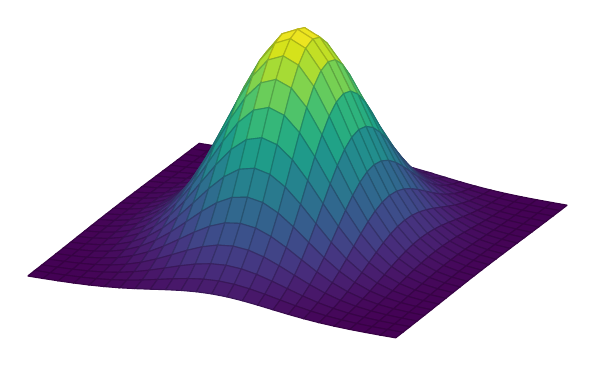
\begin{tikzpicture}
\begin{axis}[
    colormap/viridis,
  	hide axis
]
\addplot3[
    surf,
]
{(exp(-(x^2)/5-(y^2)/9))*1/4};
\end{axis}
\end{tikzpicture}
\centering
                        \includegraphics[width=200px]{pics/ellenv.png}
\caption{Representation of an ellipse (right) defined by an hyperplane intersecting the multi variate gaussian (left). Green samples are regular, red ones are outliers}
\end{figure}




\section{Dimensionality reduction}
Dimensionality reduction is a common task while dealing with datasets. It can be helpful for different reasons: time/space complexity reduction,  simpler models can be built, observability of the dataset is increased and so on. Suppose that we have datapoints with $d$ feature. If we want to reduce them to $k$ feature, we can just discard $d-k$ (\textbf{feature selection}) or we can project the original $d$ dimension to a new space with $k$ dimensions (\textbf{feature  extraction}).
Dimensionality reduction can be performed while considering the class associated to each datapoint (\textbf{supervised} or not (\textbf{unsupervised}).
\subsection{Principal Component Analysis (PCA)}
\textbf{PCA} is an \textbf{unsupervised} dimensionality reduction technique. The idea behind this method is to project datapoints into a slower-dimension space while \textbf{minimizing} the information loss. Now, consider the following assumptions:\begin{itemize}
    \item We have a dataset $\overline{X}=\{\overline{x}_1,\overline{x}_2...\overline{x}_n\}$ of $n$ datapoints, 
    \item The \textbf{dimension} of the generic datapoint $\overline{x}$ is  $\textrm{dim}(\overline{x})=d $,
    \item We wish to reduce dimension from $d$ to $k$, with $k<d$.
\end{itemize}
Therefore, we can consider the projection of $\overline{x}$ in the new space as $\overline{z}$:\[
\overline{z}=\overline{W}^\top\overline{x}
\]
Where $\overline{W}$ is  the \textbf{projection matrix}. Remember that:\[
\begin{aligned}
&\textrm{dim}(\overline{x})=d\\
&\textrm{dim}(\overline{z})=k\\
&\textrm{dim}(\overline{W})=d \times k
\end{aligned}
\]The resulting projected dataset is indicated with $\overline{Z}=\{\overline{z}_1,...\overline{z}_n\}$. The projection matrix that maximizes the \textbf{sample variance} of the dataset $Var(\overline{Z})$ is the one that minimize the \textbf{information loss}. \\ Indicating with $\overline{M}_x$ the \textbf{sample mean} of the dataset $\overline{X}$ and (with misuse of notation) with $\overline{W}^\top\overline{X}$,  the \textbf{projection} of each datapoint $\overline{x}_i\in\overline{X}$ in the new space $\overline{Z}$,we can write :\[
\begin{aligned}
Var(\overline{Z})&=Var(\overline{W}^\top\overline{X})=E\left[(\overline{W}^\top\overline{X}-\overline{W}^\top\overline{M}_x)^2\right]\\
&=E\left[\overline{W}^\top(\overline{X}-\overline{M}_x)(\overline{X}-\overline{M}_x)^\top\overline{W}\right]\\
&=\overline{W}^\top \underbrace{E\left[(\overline{X}-\overline{M}_x)(\overline{X}-\overline{M}_x)^\top\right]}_{\substack{\displaystyle\Sigma_x\\\textrm{(Covariance matrix of $\overline{X}$)}}}\overline{W}\\
\end{aligned}
\]
Remember that the \textbf{covariance matrix} represent the \textbf{variance} of a \textbf{multi-dimensional} random variable (or the \textbf{sample} variance of a set of \textbf{observations}, i.e. a dataset).
Thus, we can formalize the goal of the \textbf{PCA} as:\[
\begin{cases}
\textrm{Maximize:}\quad Var(\overline{Z})\\
\textrm{Subject to:} \quad \nrm{\overline{W}}=1
\end{cases}
\]
Now consider the vector $\overline{w}_1 \mid \textrm{dim}(\overline{w}_1)=k$ for which it holds:\[
\Sigma_x\overline{w}_1 = \lambda_1w_1
\]
Thus, $\overline{w}_1$ is an \textbf{eigenvector} for $\Sigma_x$ with $\lambda_1$ as \textbf{eigenvalue}. The eigenvector associated with the largest eigenvalue is the one along whose direction the dataset has the \textbf{highest variance}, therefore the loss of information is minimal. Thus, we can procedurally choose \textbf{eigenvectors} with decreasing \textbf{eigenvalues} (starting from the greatest) as the new basis for the space onto which we want to project the dataset. Considering that $\Sigma_x$ has $d$ eigenvectors and we have to pick the $k$ ones with the \textbf{greatest eigenvalues}, a key aspect is to evaluate how to choose $k$. A metric related to this aspect is the \textbf{Proportion of Variance Explained}, indicated with $\mathcal{P}_v$. If we consider \[
\begin{aligned}
\lambda_1>\lambda_2...>\lambda_d
\end{aligned}
\]Then $\mathcal{P}_v$  can be computed as:\[
\mathcal{P}_v=\frac{\overbrace{\lambda_1+\lambda_2+...\lambda_k}}{\underbrace{\lambda_1+\lambda_2+...\lambda_k}+\lambda_{k+1}+...\lambda_d}
\]
Typically, $k$ is chosen so as to have $\mathcal{P}_v \geq 0.9$.
\begin{figure}[H]
                \centering                       \includegraphics[width=0.80\textwidth]{pics/AI/pov.png} 
                        \caption{Eigenvectors and eigenvalues in decreasing order (a) and the value of $\mathcal{P}_v$ (b) plotted in function of $k$ (number of eigenvectors chosen for the new basis)} 
\end{figure}
\subsection{Fisher Linear Discriminant Analysis (LDA)}
\textbf{Fisher LDA} is a \textbf{supervised}   dimensionality reduction technique. In this section will be shown an example of application of \textbf{LDA} on a 2-dimensional space projected into a mono-dimensional space, but the procedure is also valid from $d$ to $k$ dimension, with $d>k$. 
Now, lets'start considering:\begin{itemize}
    \item $\overline{X}=\{(\overline{x}_i, c_i)_i\}$, with $i=1...n$ is the \textbf{dataset} made of  $n$ couples;
    \item For each couple $(\overline{x}_i, c_i)_i$ we have $\overline{x}_i \in \R^2$ which is the \textbf{observation} (datapoint) and $c_i$ which is the \textbf{class label};
    \item We have 2 possible classes $C_1$ and $C_2$. Thus, for each observation-label pair, it holds:\[
    \begin{cases}
        \overline{x}_i \in C_1\quad\longrightarrow c_i=1\\
        \overline{x}_i \in C_2 \quad \longrightarrow c_i=0 
    \end{cases}
    \]
    \item The \textbf{means} of the two sets of datapoints belonging to $C_1$ and $C_2$ are respectively $\overline{\mathcal{M}}_1$ and $\overline{\mathcal{M}}_2$.
    
\end{itemize}
The key idea behind the \textbf{LDA} is to project datapoints $\overline{x}_i$ into a new space in which the the distance between \textbf{class averages} is maximized and the \textbf{variance} of each class is minimized: with these 2 criteria we ensure that we can \textbf{distinguish} as easily as possible points belonging to different classes. Therefore, consider:\begin{itemize}
        \item $z=\overline{w}^\top\overline{x}$ is the generic datapoint projected in a \textbf{monodimensional} space, with $\overline{w}$ as \textbf{projection vector},
        \item In this new space, the \textbf{means} of the two sets of datapoints belonging to $C_1$ and $C_2$ become $\mu_1$ and $\mu_2$,
        \item In this new space, we indicate with $\sigma_1^2$ and $\sigma_2^2$, the \textbf{variances} of the two set of datapoints belonging to $C_1$ and $C_2$ respectively
    \end{itemize}
\begin{figure}[H]
                \centering                       \includegraphics[width=0.80\textwidth]{pics/AI/LDA.png} 
                        \caption{Representation of \textbf{LDA} applied for a 2-dimensional space turning into a mono-dimensional space} 
\end{figure}
Thus, we can compute:\[
\begin{aligned}
&\sigma_1^2=\sum_{\overline{x}_i\in C_1}(\overline{w}^\top\overline{x}_i-\mu_1),\quad \sigma_2^2=\sum_{\overline{x}_i\in C_2}(\overline{w}^\top\overline{x}_i-\mu_2),\\
&\phantom{aaa}\\
&\mu_1=\frac{\displaystyle\sum_{\overline{x}_i\in C_1}\overline{w}^\top \overline{x}_i}{\displaystyle\sum_{\overline{x}_i\in C_1}c_i},\phantom{aaaaaaa}
\mu_2=\frac{\displaystyle\sum_{\overline{x}_i\in C_2}\overline{w}^\top \overline{x}_i}{\displaystyle\sum_{\overline{x}_i\in C_2}(1-c_i)},\\
\end{aligned}
\]
For reasons outlined above, we can consider the following \textbf{cost function}:\[
J(\overline{w})=\frac{(\mu_1-\mu_2)^2}{\sigma_1^2+\sigma_2^2}
\]
The $\overline{w}^*$ which is a \textbf{minimum} of the \textbf{cost function} is the solution of the problem that allows us to reduce dimensionality.
\subsection{Stochastic Neighbor Embedding (SNE)}
\textbf{Stochastic Neighbor Embedding\footnote{Geoffrey Hinton and Sam Roweis, \href{https://citeseerx.ist.psu.edu/viewdoc/download?doi=10.1.1.441.8882&rep=rep1&type=pdf}{Link to the paper} }} is an \textbf{unsupervised} dimensionality reduction technique. It allows turns a $d$ dimensional space in a $k$ dimensional space, where $k$ is usually $2$ or $3$. The idea behin this approach is to \textbf{preserve} local configurations of the datapoints while \textbf{disregarding} peripheral configurations. This criteria is called \textbf{neighborhood pressuring embedding}.
\begin{figure}[H]
                \centering                       \includegraphics[width=0.50\textwidth]{pics/AI/SNE_1.png} 
                        \caption{Representation of the \textbf{neighborhood pressuring embedding} criteria. Local distances like $d_l$ and $d_l^*$ are preserved while going from $d$ to $2$ dimensions, peripheral distances like $d_p$ and $d_p^*$ are not.} 
\end{figure}
\noindent Now, consider the dataset $\overline{X}=\{\overline{x}_1,\overline{x}_2,...\overline{x}_n\}$, where each datapoint $\overline{x}$ is $d-$dimensional. At the same time, consider $\overline{Y}=\{\overline{y}_1,\overline{y}_2,...\overline{y}_n\}$ the \textbf{embedded} $2$(or $3)$-dimensional mapping of $\overline{X}$. Our goal is to define the analytical rule that allows us to \textbf{build} $\overline{Y}$ given $\overline{X}$ while respecting the \textbf{criteria} expressed before. 
\\ For each couple of points $\overline{x}_i,\overline{x}_j$ belonging to $\overline{X}$ we can define the following \textbf{elliptic conditional distribution}:\[
p_{j|i}=\frac{e^{\displaystyle\left(-\frac{\nrm{\overline{x}_i-\overline{x}_j}^2}{2\sigma_i}\right)}}{\displaystyle\sum_{k\not=i}e^{\displaystyle\left(-\frac{\nrm{\overline{x}_i-\overline{x}_k}^2}{2\sigma_i}\right)}}
\]
Where $\sigma_i$ quantifies the contribution of the \textbf{around} of $\overline{x}_i$ to the calculation. The denominator is a \textbf{normalization} term.
\noindent We can also define, for each couple $\overline{y}_i,\overline{y}_j$ the \textbf{conditional distribution}:\[
q_{j|i} = \frac{e^{\left(\displaystyle-\nrm{\overline{y}_i-\overline{y}_j}^2\right)}}{\displaystyle\sum_{k\not=i}e^{\left(\displaystyle-\nrm{\overline{y}_i-\overline{y}_k}^2\right)}}
\]
Where, again, the denominator is a \textbf{normalization} term.
The mathematical tool that allows us to find an \textbf{embedded} representation of $\overline{X}$, i.e. $\overline{Y}$, that meets the above criteria is the \textbf{Kullback-Leibler Divergence} (described in Section ...). Specifically, our goal is to find a representation $\overline{Y}$ such that the following quantity $\mathcal{C}$ is maximized:\[
\mathcal{C}=\sum_j\sum_ip_{j|i}\log\left(\frac{p_{j|i}}{p_{j|i}}\right)=\sum_i\textrm{KL}(P_i||Q_i)
\]
Therefore, we can evaluate the following \textbf{gradient}:\[
\frac{\delta \mathcal{C}}{\delta \overline{y}_i}=2\sum_j(\overline{y}_i-\overline{y}_j)(p_{j|i}+p_{i|j}-q_{j|i}-q_{i|j})
\]
There is not a solution in closed form  for the maximum of $\mathcal{C}$, but there is a non linear iterative \textbf{rule} for the estimation of the generic $\overline{y}$:\[
\overline{y}^{(t)}=\overline{y}^{(t-1)}+\psi \frac{\delta \mathcal{C}}{\delta \overline{y}}+\alpha\left(\overline{y}^{(t-1)}-\overline{y}^{(t-2)}\right)
\]
Where:\begin{itemize}
    \item $\psi$ is called \textbf{learning hyperparameter}, and regulate the weight of the gradient. This parameter is \textbf{mandatory}.
        \item $\alpha$ is the \textbf{difference hyparameter}, that regulate the weights of the values in the previous iterations. This parameter is \textbf{not} mandatory(i.e. it can be $0$).

\end{itemize}
\section{Introduction to Deep Learning} 
Artificial neural networks (ANNs), usually simply called neural networks (NNs), are computing systems inspired by the biological neural networks that constitute animal brains.\textbf{Deep learning} is the discipline that studies different neural network architectures. 
A generic NN is based on a collection of \textbf{connected units} or nodes, which loosely model the \textbf{neurons} in a biological brain. Each connection, like the synapses in a biological brain, can transmit a signal to other neurons. An artificial neuron that receives a signal then processes it and can signal neurons connected to it.
\begin{figure}[H]
                \centering
                        \includegraphics[width=0.75\textwidth]{pics/AI/Neuron3.png} 
                        \caption{Biological structure of neurons that inspires the architecture of neural networks. Each neuron has $n$ inputs coming from \textbf{dendites}. The output is propagated through $m$ \textbf{axon terminals}} 
\end{figure}
\noindent 
A neural network usually has $\approx10^5$ connection per processing unit (neuron), that are $\approx 10^{10}$, resulting in a total of $10^{15}-10^{18}$ connections. This kind o architecture grants \textbf{noise-failure robustness} while distributing computation/memory and allowing parallel processing. 
There are many architectures and models of neural networks, which are used to solve the a lot of different tasks. Research in this field is quite fervent and new architectures are being designed all the time. The family of models that has historically had the most importance is that of the \textbf{Convolutional Neural Networks} (CNN), contextualised to the \textbf{image classification} task (recent studies have documented the possibility of adapting them also to solve other tasks).
\subsection{Perceptron}
The smallest processing unit used in many neural networks (including CNNs) is the \textbf{Rosenblatt's perceptron}.
This unit is capable of solving \textbf{linearly separable problems}.
In order to describe it, consider:\begin{itemize}
    \item $\overline{x}_{IN}={[x_1,x_2...x_N]^\top}$ as the \textbf{input vector},
    \item The constant $x_0=1$, useful to introduce the \textbf{bias term}. Note that $x_0$ \textbf{is not} part of the input vector, it's just introduced in order to simplify notation.
    \item  In accordance with the previous notation, we can write then $\overline{x}=[x_0,\overline{x}_{IN}]^\top$. Thus, $\overline{x}$ contains the constant $x_0=1$ and the elements of the \textbf{input vector},
    \item $\overline{w}={[w_0,w_1...w_N]^\top}$ is the \textbf{weight vector}, where $w_0$ is the \textbf{bias term}. Note that $\text{dim}(\overline{w})=\text{dim}(\overline{x})=N+1$,
    \item The model of the "cell body" perform a sum of the components of the \textbf{input vector}, weighted by the \textbf{weight vector}, plus the \textbf{bias term}. In accordance with this notation we can write: \[
    \sum_{\textcolor{red}{j=1}}^N\underbrace{w_jx_j}_{\substack{\textrm{weighted}\\\textrm{input}}}+\underbrace{x_0w_0}_{\substack{\textrm{bias term,}\\\textrm{n.b $x_0=1$}}}=\overline{w}^\top\overline{x}
    \]
    \item The outoput $y$ is regulated by an \textbf{activation function} $f_{att}$ that takes as input the \textbf{sum} performed by the "cell body". This output is sent to the other perceptrons and it will be a component ofthe input vector of those perceptrons. We can write then:\[
    y=f_{act}(\overline{w}^\top\overline{x})
    \]
\end{itemize}
\begin{figure}[H]
                \centering
                        \includegraphics[width=0.85\textwidth]{pics/AI/perceptron.png} 
                        \caption{Rosenblatt's perceptron} 
\end{figure}
There are different functions that can be used as activation function. Usually, the activation function is satutrated between 2 values that indicated whether the perceptron is sending signal or not.
\fastpic{pics/AI/actvfunct.png}{Different activation functions. The nonlinearity introduced by these functions is fundamental to the final behaviour of the entire architecture}{1}
\begin{comment}
\begin{figure}[H]
    \begin{tikzpicture}
	\begin{axis}[
		xlabel=$x$,
		ylabel={sigmoid}
	]
	    \addplot[mark=none,color=red,domain=-8:8] {1/(1+e^(-x))};
	    \end{axis}
    \end{tikzpicture} 
    \begin{tikzpicture}
	\begin{axis}[
		xlabel=$x$,
		ylabel={tanh}
	]
	    \addplot[mark=none,color=red,domain=-8:8] {tanh(x)};
	    \end{axis}
    \end{tikzpicture}    
    \begin{tikzpicture}
	\begin{axis}[
		xlabel=$x$,
		ylabel={linear function}
	]
\addplot[domain=-9:-2,red]{0};
\addplot[domain=-2:3,red]{(x+2)/5};
\addplot[domain=3:9,red]{1};

\end{axis}
    \end{tikzpicture}    
    \begin{tikzpicture}
	\begin{axis}[
		xlabel=$x$,
		ylabel={step function}
	]
\addplot[domain=-9:9,red]
{
(x<=0) * 0 +
(x>0)  * 1
};
\end{axis}
    \end{tikzpicture}    
    \begin{tikzpicture}
	\begin{axis}[
		xlabel=$x$,
		ylabel={ReLu}
	]
    \addplot[domain=-9:0,blue]{0};
    \addplot[domain=0:9,blue]{x/2};	    \end{axis}
    \end{tikzpicture}    
    \caption{Different activation functions. On the y axis, the name of the function} 
\end{figure}
\end{comment}


\noindent The perceptron can be used to solve \textbf{both} simple linear regression and classification for linearly separable problems with 2 classes.

For regression problems, suppose having:\begin{itemize}
    \item A dataset $\mathcal{D}=\{(\overline{x}^{(t)}_i,r^{(t)}_i)\}$, $i=1...D$ where each pair is made by an input vector $\overline{x}^{(t)}_i$ and real value $r^{(t)}_i\in \R$ as output. The $(t)$ stands for \textbf{training}
    \item Without loss of generality, assume having a \textbf{ReLu} as activation function, thus\[
y=\textrm{ReLu}(\overline{w}^\top\overline{x})=\begin{cases}
    0 \quad\textrm{for:  }\overline{w}^\top\overline{x}<0  \\
    k\overline{w}^\top\overline{x} \quad\textrm{for:  }  \overline{w}^\top\overline{x} \geq 0
\end{cases}
\]
\item A cost function $L(\overline{w})$. For this example assume an $L_2$ distance without loss of generality:\[
L(\overline{w}) = \sum_{i=1}^D\frac{1}{2}\left(\overline{w}^\top\overline{x}^{(t)}_i-r^{(t)}_i\right)^2
\]
That measures the distance between the \textbf{labeled value} and the \textbf{predicted outcome}.
\end{itemize} 
The goal then is to find the $\overline{w}^*$ such that:\[
\overline{w}^*=\underset{\overline{w}}{\textrm{argmin}}\left[L(\overline{w})\right]
\]
In order to do it, we need to compute $\nabla_{\overline{w}}\left[L(\overline{w})\right]$ from the cost function, then we can use the following \textbf{iterative rule}:\[
\begin{aligned}
&\overline{w}^{(0)}=\textrm{random}\\
&\overline{w}^{(k)}=\overline{w}^{(k-1)}+\eta\left[L(\overline{w}^{(k-1)})\right]
\end{aligned}
\]
Where $\eta$ is the \textbf{learning hyperparameter} and $k$ is the \textbf{step} of the iteration.
This method is called \textbf{gradient descent}. \\
The perceptron can also be used to solve classification tasks with 2 classes that are linearly separable. Assume that we have:\begin{itemize}
    \item A perceptron that handles $\overline{x}_{IN}=[x_1,x_2...x_N]^\top$ as \textbf{input vector}, where $x_0=1$ is used to introduce the bias (according to the notation used previously), 
    \item As previously, $\overline{x}=[x_0,\overline{x}_{IN}]$,
    \item A \textbf{weight vector} $\overline{w}=[-\theta,w_1,w_2...w_N]^\top$ , where $\theta$ is the \textbf{bias term},
    \item Assume $\textrm{Step}(x)$ as \textbf{activation function} for this example:\[
    \textrm{Step}(x)=\begin{cases}
        0 \quad\textrm{for}\quad  x<0\\
        1 \quad\textrm{for}\quad  x\geq0
    \end{cases}
    \]
\end{itemize}

\begin{figure}[H]
                \centering
                        \includegraphics[width=0.70\textwidth]{pics/AI/classperc.png} 
                        \caption{Representation of a perceptron used in a classification task. Observe  how the components of $\overline{x}$ affect the output: the \textbf{bias term} $\theta$ regulates the \textbf{threshold} and the weighted sum of the \textbf{input vector} appears as variable on the $x$ axis} 
\end{figure}
\noindent Thus, the output $y$ will be:\[
y(\overline{x})=\textrm{Step}(\overline{w}^\top\overline{x})
\]
If we consider the output as function the \textbf{input vector} only, $\overline{x}_{IN}=[x_1,x_2...x_N]^\top$ we can see that we have:\[
y(\overline{x}_{IN})=\begin{cases}
    0 \quad \textrm{for: } \quad \displaystyle\sum_{\textcolor{red}{j=1}}^Nx_jw_j<\theta\\
    1 \quad \textrm{for: } \quad \displaystyle\sum_{\textcolor{red}{j=1}}^Nx_jw_j\geq\theta
\end{cases}
\]
Thus, we can write:\[
y=\textrm{Step}_{\theta}\left(\sum^N_{j=1}x_jw_j\right)
\]
where $\textrm{Step}_\theta(x)$:\[
\textrm{Step}_\theta(x)=\begin{cases}
    0 \quad \textrm{for: } \quad x<\theta\\
    1 \quad \textrm{for: } \quad x\geq\theta
\end{cases}
\]
We can see that we have defined a \textbf{separation hyperplane} between \textbf{input vectors} whose weighted sum \textbf{exceeds} $\theta$ and those whose not. The output of the perceptron will be 1 having the first ones 1 as input and 0 with the others.  Again, the best choice of $\overline{w}$ is found iteratively with the   \textbf{Gradient Descent} technique.
\begin{figure}[H]
                \centering
                        \includegraphics[width=0.80\textwidth]{pics/AI/classperc2.png} 
                        \caption{Graphical representation of the hyperplane defined by a classification perceptron. Remind similarities with the SVM.}
\end{figure}
\subsection{Fully connected layer}
If we wish to solve a multi-regression or a \textbf{k-classes} classification problem, we can use the \textbf{fully connected} configuration. For a $K$ class classification or a K-values regressions, we have $K$ perceptrons, where each one receives all the components of $\overline{x}$ as input. In order to describe this configuration, let's consider:\begin{itemize}
\item $\overline{x}_{IN}=[x_1,x_2...x_N]^\top$ as \textbf{input vector} and $\overline{x}=[x_0,x_1...x_N]^\top$, with $x_0=1$
\item $\overline{\gamma}=[\gamma_1,\gamma_2...\gamma_K]^\top$ the vector that contains the \textbf{activity level} $\gamma_j$ of each perceptron.
\item A \textbf{weight matrix} $\overline{W}^{(N+1)\times K}$ the regulates the weighted relationship between the $N$ features of the input vector (+ $x_0=1$ for the bias regulation) and the $K$ perceptrons,
\item The output vector $\overline{y}=[y_1,y_2...y_K]$
\end{itemize}
 Each row vector $\overline{w}_n^{(r)}=[w_{n0},w_{n1}...w_{nK}],\,\,n=1...N$ contains the weights for a given feature $x_n$  when acting as input for each one of the $K$ perceptrons. The row vector  $\overline{w}_0^{(r)}=\overline{\theta}$ is the vector that contains the \textbf{bias terms} (i.e. the weights for the input feature $x_0=1$). Remind that $x_0=1$ in order to introduce the bias in a perceptron. Vice-versa, each column vector $\overline{w}_k^{(c)}=[w_{0k},w_{1k}...w_{Nk}]^\top$ describes the weights that the $k$-th \textbf{perceptron} associates with the \textbf{input vector}. Therefore, each \textbf{scalar weight} $w_{nk}$ represents \textbf{the weight of the connection} between the input $x_n$ and the $k-$th perceptron. \[
 \overline{W}^{(N+1)\times K}=
 \begin{blockarray}{*{5}{c} l}
    \begin{block}{*{5}{>{\footnotesize}c<{}} l}
      \overline{w}_1^{(c)} & \overline{w}_2^{(c)} & \overline{w}_3^{(c)} &  & \overline{w}_K^{(c)} & \\
    \end{block}
    \begin{block}{[*{5}{c}]>{\footnotesize}l<{}}
      \textcolor{blue}{w_{01}} & \textcolor{blue}{w_{02}} & \textcolor{blue}{w_{03}} & \textcolor{blue}{...} & \textcolor{blue}{w_{0K}}\bigstrut[t]&\textcolor{blue}{\overline{w}_0^{(r)}=\overline{\theta}} \\
w_{11} & w_{12} & w_{13} & ... & w_{1K}& \overline{w}_1^{(r)}\\
...&...&...&w_{nk}& ...& \\
w_{N1} & w_{N2} & w_{N3} & ... & w_{NK}& \overline{w}_N^{(r)}\\
\end{block}
  \end{blockarray}
 \]
\begin{figure}[H]
                \centering
                        \includegraphics[width=0.75\textwidth]{pics/AI/fully.png} 
                        \caption{Representation of a \textbf{fully connected} layer. Each $\overline{w}_K^{(c)}$ represent the weights that each perceptron gives to each input. Thus, each scalar weight $w_{nk}$ represents t\textbf{he weight of the connection} between the input $x_n$ and the $k-$th perceptron} 
\end{figure}
\noindent Thus, we can write:\[
\begin{aligned}
&\overline{\gamma}=\overline{W}^\top\overline{x};\\
&\gamma_k=\overline{w}_k^{(c)\top}\overline{x}
\end{aligned}
\]
It's common to have an activation function that regulates the output acording to the activity level.
In the example, each output $y_k$ (i.e. the whole \textbf{output vector}) is regulated by the \textbf{SoftMax} function, that is:\[
y_k=\frac{e^{\gamma_k}}{\displaystyle\sum_{k=1}^Ke^{\gamma_k}}
\]
There are different ways to manage a K-class classification problem, for example we can consider the output class as $C_k$ when:\[
C_k\quad\textrm{if }\quad y_k=\underset{K}{\text{max}}(y_k)
\]
Or we can also use the \textbf{one-hot encoding} to represent classes: the k-th class membership is represented by a vector $\overline{r}$:\[
\overline{r}\in C_k\longrightarrow\begin{cases}
    r_i=0 \quad\textrm{if }\quad i\not=k\\
    r_i=1 \quad\textrm{if }\quad i=k
\end{cases}
\]
Thus, we can use \textbf{one hot encoded} vectors as labels for \textbf{training set} while placing an activation functions that gives 1 for $y_k=\underset{K}{\text{max}}(y_k)$ and 0 otherwise.\\
The weight matrix $\overline{W}$, again, is found using the \textbf{gradient descent} technique suitably adapted to the \textbf{fully connected} architecture.
Suppose to have a training set $\mathcal{D}=\{(\overline{x}^{(t)},\overline{r}^{(t)})^{(t)}\}$ made of $T$ pairs.
Each pair is made by the \textbf{datapoint} $\overline{x}^{(t)}\,,\textrm{dim}(\overline{x}^{(t)})=N$ and the label vector $\overline{r}^{(t)}\,,\textrm{dim}(\overline{r}^{(t)})=K$ that represents the \textbf{ground truth}. The value $(t)$ indicates the index of the training sample, which means that $t\in\{1,2,...T\}$. Suppose for simplicity that the output of the k-th perceptron is $y_k=\gamma_k$, (the \textbf{activity level} is the output, i.e. we have no activation function). We can define a \textbf{cost function}, which can be evaluated for any training entry  $(\overline{x}^{(t)},\overline{r}^{(t)})$, :\[
\frac{1}{2}L_t(\overline{W})=\sum_{k=1}^K\left(r_k^{(t)}-y_k\right)^2
\]
It represent, for any training sample $(t)$, the sum of the $K$ \textbf{distances} between the $K$ components $r_k^{(t)}$ of the \textbf{ground truth} and the corresponding output of the K perceptrons $y_k$. Remember that, for assumption:\[
y_k=\gamma_k=\overline{w}_k^{(c)\top}\overline{x}
\]
Thus, we can compute the following \textbf{derivative}:\[
\frac{\partial L_t(\overline{W})}{\partial w_{nk}}=\nabla L_t(w_{nk})=(r_k^{(t)}-y_k)x_n^{(t)}
\]
Therefore, we can write the \textbf{gradient descent} rule for this case:\[
    \begin{aligned}
        &w_{nk}^{(0)}=\textrm{random};\\
        &w_{nk}^{(m+1)}=w_{nk}^{(m)}-\eta\nabla L_t(w_{nk}^{(m)})
    \end{aligned}
\]
The last term is the \textbf{update term} and can be seen as: \[
\begin{aligned}
&\eta\nabla L_t(w_{nk}^{(m)})=\eta(r_k^{(t)}-y_k)x_n^{(t)}\\
=\text{LearnFactor}&\textrm{(Desired Output-Actual Output)Input}
\end{aligned}
\]

\noindent As we said, our dataset has $T$ pairs of entries. There are 2 ways to use this data for learning:\begin{itemize}
    \item \textbf{Online learning}.\\ 
    In this approach we provide \textbf{one entry at time}, and for each one we perform a complete \textbf{update loop}: we compute the $\nabla L_t(w_{nk}^{(m)})=(r_k^{(t)}-y_k)x_n^{(t)}$ (n.b. $t$ represent the training entry pair ), and then we can apply the \textbf{gradient descent} rule in order to update the $w_{nk}^{(m+1)}$ of the \textbf{weight matrix}
    \item \textbf{Batch learning}:\\
    In this approach we provide the \textbf{entire dataset} all at once: the \textbf{update term} is computed for each entry but it is \textbf{averaged} before to apply the \textbf{gradient descent} update rule. The presentation of the entire dataset is called \textbf{epoch}, and usually more epochs are required in order to obtain the convergence of $\overline{W}$.
\end{itemize} 
 Convergence is considered to have been achieved when the loss is less than a certain value ($10^{-3}$) or when the weights $w_{nk}$ do not change from one epoch to the next. 
\subsection{MLP Layer}
As we saw, with a single perceptron we can solve simple \textbf{linear problems}: linear regressions and 2-class classification problems. With the \textbf{fully connected} layer the complexity of the problems that can be solved grows: we can solve multi regressions and k-class classification problems.
The solution method is the same in both cases: using iterative \textbf{gradient descent} techniques, the weight matrix/vector that minimizes the \textbf{cost function} is sought.
A single perceptron, if properly configured, can simulate an OR or an AND function. But this cannot be done for the XOR function, that is a non linear one. Non-linear problems can be solved by the  \textbf{Multi-Layer-Perceptron (MLP)} layer.
\begin{figure}[H]
                \centering
                        \includegraphics[width=0.8\textwidth]{pics/AI/multiLayer.png} 
                        \caption{\label{fig:mlp:arch}Representation of a \textbf{Multi-layer} perceptron. The weight $w_{nh}$ regulates the connection between the n-th input and the h-th perceptron of the hidden layer, whereas the $v_{hk}$ weight regulates the connection between the h-th perceptron of the hidden layer and the k-th perceptron of the output layer.} 
\end{figure}
\noindent In this schema, we have the following components:\begin{itemize}
    \item The \textbf{input vector}: as always, we have $x=[x_0,x_1...x_N]$, where $x_0=1$.
    \item The \textbf{hidden layer}: this layer is made of $H$ perceptrons. The connection between the n-th \textbf{input} and the h-th \textbf{hidden perceptron} is regulated by the weight $w_{nh}$. Thus, we have a $\overline{W}^{(N+1)\times H}$ weight matrix (the +1 is required for the bias). After the weighted sum, the activity value is fed to an \textbf{activation function} ($f_{act1}(\cdot)$ in the schema) that produces the \textbf{output} of this layer, called $z_h$ for the h-th perceptron. 
    \item The \textbf{output layer}, that is similar to the hidden layer: this layer is made of $K$ perceptrons. The connection between the h-th peceptron of the \textbf{hidden layer} and the k-th \textbf{output perceptron} is regulated by the weight $v_{hk}$. Thus, we have a $\overline{V}^{(H+1)\times K}$ weight matrix (the +1 is required for the bias) . After the weighted sum, the activity value is fed to an \textbf{activation function} ($f_{act2}(\cdot)$ in the schema) that produces the \textbf{output} of this layer, called $y_k$ for the k-th perceptron. 
\end{itemize}

%\begin{figure}[H]
%                \centering
%                        \includegraphics[width=0.6\textwidth]{pics/AI/PercLayers.png} 
%                        \caption{A possible implementation of the 2 activation %functions} 
%\end{figure}
\noindent In this configuration, the activation functions are the \textbf{hyperparameters} of the system, while the weight matrices are the \textbf{parameters}.\\
In accordance with this notation, the  output of the h-th perceptron of the \textbf{hidden layer } $z_h$ will be:\[
z_h=f_{act1}\left(\overline{w}_h^{(c)\top}\overline{x}\right)
\]
Remind that:\[
\overline{w}_h^{(c)\top}\overline{x}=\sum_{n=1}^Nw_{hn}x_n+w_{h0}
\]
Consequently, the  output of the k-th perceptron of the \textbf{output layer} $y_k$ will be:\[
y_k=f_{act2}\left(\overline{v}^{(c)\top}_k\overline{z}\right)
\]
Again, remind that:\[
\overline{v}^{(c)\top}_k\overline{z}=\sum_{h=1}^Hv_{kh}z_h+v_{k0}
\]
It should be noted that since the two activation functions have no linearity constraint, the \textbf{MLP} is highly \textbf{non-linear} and can solve even non linearly separable problems.
\begin{figure}[H]
                \centering
                        \includegraphics[width=0.7\textwidth]{pics/AI/nonLin.png} 
                        \caption{The MLP can solve non linear problems. It can correctly classify and infer information coming from datasets like above, that are clearly non-linear.} 
\end{figure}
\noindent The architecture presented in this paragraph, in which we have in cascade \textbf{input} layer - \textbf{hidden} layer - \textbf{output} layer is only a possible implementation of a MLP schema: there is \textbf{no universal rule} that defines the \textbf{number} and \textbf{size} of the \textbf{hidden} layers interspersed \textbf{between} the \textbf{input} and the \textbf{output} layer, usually the design of the layers is done \textbf{empirically} and specific to the case study. When hidden layers tend to generate outputs that are dimensionally \textbf{smaller} than the input they receive they are called \textbf{embdedding} layers. Vice versa, they're called \textbf{expansion} layers.
\subsection{Convolution layer}
This layer is typical (but not only) of \textbf{CNN}s. In \textbf{image-classssification}, it plays a fundamental role in that it makes it possible to recognise \textbf{patterns} and \textbf{structures} typical of certain \textbf{classes} that one wishes to identify (for example, the presence of a certain animal species).
The \textbf{convolution layer} is so called because it performs \textbf{convolution} between the \textbf{input} and one or more \textbf{filters}. Let's start by defining the \textbf{Hadamard product}:
\begin{customTheo}\textbf{Hadamard product}:\\
The \textbf{Hadamard product} $\odot$ is an operation between two matrices having the \textbf{same dimension},. If assume $A^{n\times m}$ and $B^{n\times m}$, $A \odot B$ can be defined as:\[
A \odot B = \begin{bmatrix}
a_{11}b_{11} && a_{12}b_{12} & ... & a_{1n}b_{1n} \\
a_{21}b_{21} && a_{22}b_{22} & ... & a_{2n}b_{2n} \\
... && ... & ... &... \\
a_{m1}b_{m1} && a_{m2}b_{m2} & ... & a_{mn}b_{mn} \\
\end{bmatrix}
\]
\end{customTheo}
\noindent
For ease of exposition and notation, suppose the input is an \textbf{image}. Consider an image as a matrix of scalar $X$:\[
X:=\begin{bmatrix}
x_{11} & x_{12} & ... &x_{1J}\\
x_{21} & x_{22} & ... &x_{2J}\\
... & ... & ... &...\\
x_{I1} & x_{I2} & ... &x_{IJ}\\
\end{bmatrix}
\]
Consider a \textbf{convolution filter} of \textbf{radius} $r$ as the matrix of scalars $W^{(r)}$:\[
W^{(r)}:=\begin{bmatrix}
w_{11} & w_{12} & ..  & w_{1R}\\
w_{21} & w_{22} & ... &w_{2R}\\
... & ... & ... &...\\
w_{R1} & x_{R2} & ... &x_{RR}\\
\end{bmatrix}
\]
Where $R=2r+1$. Assume $R$ always \textbf{odd} for simplicity of notation, without loss of generality.
The \textbf{convolution} between $X$ and the filter $W^{(r)}$ is done as follows:\begin{itemize}
    \item For each component $x_{ij}$, choose an \textbf{around} from $X$ \textbf{centered} $x_{ij}$ of \textbf{radius} $r$, that is  a \textbf{matrix} of size $R=2r+1$ (same as $W^{(r)}$), called $I^{(r)}_{ij}$. 
    \item \textbf{Compute} $H_{ij}^{(r)}=W^{(r)}\odot I_{ij}^{(r)}$.
    \item \textbf{Sum} all the components of $H_{ij}^{(r)}$, the result will be a \textbf{scalar} called $h^{(r)}_{ij}$.
\end{itemize}
\begin{figure}[H]
                \centering
                        \includegraphics[width=0.4\textwidth]{pics/AI/convolution.png} 
                        \caption{
Diagram of the procedure for obtaining the components of an \textbf{activation map}. }
\end{figure}
The resulting matrix composed of the various $h^{(r)}_{ij}$, let's  simply say $Y$, is called  \textbf{activation map}. Note that the filter is \textbf{invariant} during the convolution. Anyway, more filters can be used to obtain more \textbf{activation maps}. 
While working in practice with images, we have to handle 3 input matrices, because we have 3 \textbf{color channels}. The convolution between the \textbf{3-channel }image and a given filter $W^{(r)}$ will still produce only one \textbf{activation map}, which will be the result of the \textbf{sum} of the \textbf{individual} activation maps obtained from the simple convolution between the \textbf{filter} and \textbf{each one} of the 3 \textbf{colour channels} matrices.
\begin{figure}[H]
                \centering
                        \includegraphics[width=0.9\textwidth]{pics/AI/convolution_2.png} 
                        \caption{
Convolution between a given filter (not shown) with an image with 3 color channels. The yellow one is the final \textbf{activation map} }
\end{figure}
\noindent Thus, a \textbf{convolution layer} implements the convolution between the \textbf{input} (suppose an image) and more filters, each one giving as result a single activation map. 
The scalar values contained in the filters are \textbf{parameterised}: during the \textbf{backpropagation} phase, the parameters of the filters will be selected so as to optimise the loss function. This will bring out the filters that best isolate the \textbf{micro/macro structures} with the most information for our problem. 
A convolution layer usually has 4 basic \textbf{hyperparameters}: \begin{itemize}
\item The number of filters to be applied, $n_f$,
    \item The \textbf{size} of the \textbf{filter} $R$, described previously,
    \item The \textbf{stride} $s$: this parameter indicates the \textbf{"jump"} to be made in choosing an $x_{ij}$ component on which to build the \textbf{neighbourhood} on which to apply the \textbf{filter}. In the examples discussed so far, the \textbf{stride} was always 1. \textbf{At each iteration}, with a stride of $s$, we \textbf{move} $s$ pixels and construct the next neighbourhood. You can also specify a different \textbf{vertical} stride $s_v$ and a different \textbf{horizontal} stride $s_h$,
    \item The \textbf{Padding} $p$: a padding of $p$ adds a \textbf{"border"} of $p$ pixels to the input of the convolution layer. Padding pixels contain an \textbf{arbitrary} value (usually $0$). In the absence of \textbf{padding}, it is \textbf{impossible} to select a \textbf{neighbor} for pixels that are on the \textbf{edge} of the image. \textbf{Padding} allows neighbor to be chosen for those pixels as well. It is called \textbf{full padding} when it is set so that the pixels on the \textbf{outermost edge} can also be analysed.
\end{itemize}
Once these \textbf{hyper-parameters} have been set, it is possible to calculate both the total \textbf{number} of parameters in the layer and the \textbf{size} of the output activation maps, (knowing the size of the input). 
To know the total number of parameter of a layer, it's sufficient to know $R$ and $n_f$:\[
\#(\text{parameters})= n_f(3R^2+1) 
\]
This formula is valid for an \textbf{image processing} problem: the 3 represent the \textbf{channels}. We also have the \textbf{bias} parameter (the $+1$).
Assuming an input image $N\times N\times3$, an activation map generated by a \textbf{single} filter will have size $K$:\[
K=\frac{N+p-R}{s}+1
\]
Thus, if we apply $n_f$ \textbf{filters}, the \textbf{output} $Y$ of a convolution layer  will have \textbf{dimension}:\[
\textrm{dim}(Y)=K\times K \times n_f
\]
This means that $n_f$ becomes the new \textbf{channel size}.
It is common practice to cascade \textbf{several} \textbf{convolution} layers, gradually \textbf{increasing} the number of filters and thus the '\textbf{depth}' (or 'number of channels') of the output. The channels then \textbf{stop} representing colours and begin to represent the \textbf{number} of \textbf{activation} \textbf{maps} generated by the previous layer. Since the single filter must be applied to \textbf{each} channel and the various results are then \textbf{combined} into a \textbf{single} activation map, conventionally the third dimension of the filter is indicated \textbf{consistently} with the \textbf{depth} of the channels, even if the filter can be seen as \textbf{two-dimensional}. 
\begin{figure}[H]
                \centering
                        \includegraphics[width=1\textwidth]{pics/AI/convolution_3.png} 
                        \caption{
Diagram representing the input and output \textbf{sizes} of various cascaded \textbf{convolution} \textbf{layers}. It is evident that the depth of the \textbf{filters} must be consistent with the depth of the \textbf{input}, while the depth of the \textbf{output} equals the number of \textbf{activation maps} generated (and therefore the \textbf{number} of different \textbf{filters} used).}
\end{figure}
\noindent A special case of convolution is with a $1\times1$ filter, \textbf{padding} $p=0$ and \textbf{stride} $s=1$.
Assuming we have a volume of size $H\times W \times D$ as \textbf{input}, the \textbf{output} of the convolution just described will be an \textbf{activation map} $H\times W \times 1$.
This operation can be seen as a \textbf{fully connected configuration} that acts on the \textbf{depth} of the data: the pixel of coordinate $H,W$ of the output map will represent the \textbf{weighted sum} of the $D$ pixels in the input volume had the \textbf{first two} coordinates $H,W$.
The weights in this case are represented by the $D$ components of the $1\times1\times D$ filters.
This technique is widely used (for example in \textbf{inception networks}) to strategically \textbf{resize} data at certain points in the network: using $D^*$ filters that perform the operation just described, as many activation maps are generated, therefore the input volume is \textbf{resized} \textbf{from} $H\times W\times D$ \textbf{to} $H\times W\times D^*$

\begin{figure}[H]
                \centering
                        \includegraphics[width=0.8\textwidth]{pics/AI/shrink.png} 
                        \caption{
Diagram representing the input and output \textbf{sizes} of a \textbf{resizing} convolution layer}
\end{figure}
\subsection{Transposed convolutional layer (TODO)}
\subsection{Pooling layer}
The \textbf{pooling layer} is a type of \textbf{layer} that \textbf{downsamples} the input. In addition to the intuitive \textbf{performance} advantages (the size of the input \textbf{decreases}), it makes \textbf{pattern detection} more robust. The pooling layers \textbf{do not} have trainable parameters, they have only the \textbf{hyper-parameters} $R$, $s$ and $p$, related respectively to the \textbf{dimension} of the observation window, the \textbf{stride} and the \textbf{padding} (\textbf{full padding} is a common choice). As we did for the \textbf{convolution}, for ease of notation, suppose the input is an \textbf{image}. Consider \textbf{each channel} of an image as a matrix of scalar $X$:\[
X:=\begin{bmatrix}
x_{11} & x_{12} & ... &x_{1J}\\
x_{21} & x_{22} & ... &x_{2J}\\
... & ... & ... &...\\
x_{I1} & x_{I2} & ... &x_{IJ}\\
\end{bmatrix}
\]
Then, consider a pooling \textbf{observation window} of size $R\times R$, where $R=2r+1$. Assume $R$ always \textbf{odd} for simplicity of notation, without loss of generality.
For \textbf{each} channel, the pooling phase consist in the following operations: \begin{itemize}
    \item For certain components $x_{ij}$ (according to the stride parameter $s$, all of them when  $s=1$ with a \textbf{full padding}), choose an \textbf{around} from $X$ \textbf{centered} in $x_ij$ of the \textbf{same size} of the observation window ($R\times R$). 
    \item To this $R\times R$ \textbf{around-matrix}, apply a function $\phi: \R^{R^2}\longrightarrow   \R$ that returns a \textbf{single} scalar value $h_ij$,
    \item As we did in the convolution, build a new matrix (a new \textbf{channel}) with all the $h_{ij}$.
\end{itemize}
\textbf{Unlike} convolution, the output matrices generated by each channel \textbf{are not} summed into a single activation map, but are kept \textbf{separate}. For this reason, the depth of the output will always be \textbf{consistent} with that of the input (note that in the case of pooling the observation window has \textbf{no} depth).
A common choice for the $\phi$ function is the  $\textrm{max}(\cdot)$ function, that return the \textbf{maximum} of the $R\times R$ scalars. In this case, the layer is called \textbf{max-pooling}. Another choice could be the \textbf{average} function, in this case we talk about \textbf{average pooling}.
\begin{figure}[H]
                \centering
                        \includegraphics[width=0.6\textwidth]{pics/AI/pooling.png} 
                        \caption{
Diagram representing the operation performed by a \textbf{pooling layer}, with \textbf{window} \textbf{size} $3\times 3$}
\end{figure}


\subsection{Backpropagation}
Even in the most complex architectures, the optimisation of the parameters of a neural network (the \textbf{weight matrices}) is often based on \textbf{iterative gradient-based} techniques. When more than one layer is present, we speak of \textbf{backpropagation}. Let's consider, for example, the schema in (Figure \ref{fig:mlp:arch}) of a \textbf{MLP}. With that configuration, a possible cost function could be:\[
\begin{aligned}
\label{eqn:bck:loss}
J(\overline{W},\overline{V})&=\sum_{t=1}^T\sum_{k=1}^K\frac{1}{2}(y_k^{(t)}-r_k^{(t)})^2\\
&=\sum_{t=1}^T\frac{1}{2}\nrm{\overline{y}^{(t)}-\overline{r}^{(t)}}^2
\end{aligned}
\]
Which we can refer to as $J$ \textbf{for simplicity of notation}. In the previous statement:\begin{itemize}
    \item $\overline{W},\overline{V}$ are the \textbf{weight matrices},
    \item The index $t\in\{1,2...T\}$ represents the entry of the \textbf{labeled dataset}. Each one of the $T$ entries is a pair $\{\overline{x}^{(t)},\overline{r}^{(t)}\}$ where $\overline{x}^{(t)}$ is the \textbf{datapoint} and $\overline{r}^{(t)}$ is the \textbf{label} (ground truth)
    \item With misuse of notation, in order to simplify reading, we shall denote by $\overline{y}^{(t)}$ the \textbf{output vector} returned by the system having $\overline{x}^{(t)}$ as input.  

\end{itemize}
\begin{figure}[H]
                \centering
                        \includegraphics[width=0.8\textwidth]{pics/AI/backprop.png} 
                        \caption{\label{fig:bp:costJ}
Diagram that represents how the cost function $J$ is obtained. In this case, $J$ is function of the two weight matrices $\overline{V}$ and $\overline{W}$.Thus $J$ is the shortened notation of $J(\overline{W},\overline{V})$ }
\end{figure}
Anyway, for the following analysis, \textbf{we can omit the supescript} "$(t)$" \textbf{without loss of generality}, since the following reasoning is valid for all datapoint-label pairs \textbf{regardless of their index}.
Let's give a look to the last layer by considering an iterative rule for the weight matrix $\overline{V}$:
\[
\overline{V}^{(m+1)}=\overline{V}^{(m)}+\Delta\overline{V}
\]
The update term $\Delta\overline{V}$ is :\[
\Delta\overline{V}=-\eta_v\nabla_{\overline{V}}[J]
\]
Where:\begin{itemize}
    \item $\eta_v$ is the \textbf{learning hyperparameter} ,
    \item $\nabla_{\overline{V}}[J]$ is a matrix with the \textbf{same dimension} of $\overline{V}^{(H+1)\times K}$ , that describes how much $J$ varies as the individual component $v_{hk}$. Its explicit representation is:\[
    \nabla_{\overline{V}}[J]=
\begin{bmatrix}
\displaystyle\frac{\partial J}{\partial v_{01}} & \displaystyle\frac{\partial J}{\partial v_{02}}  &...& \displaystyle\frac{\partial J}{\partial v_{0K}}\\
\displaystyle\frac{\partial J}{\partial v_{11}} & \displaystyle\frac{\partial J}{\partial v_{12}} & ...& \displaystyle\frac{\partial J}{\partial v_{1K}}\\
...&...&\displaystyle\frac{\partial J}{\partial v_{hk}}&...&\\
\displaystyle\frac{\partial J}{\partial v_{H1}}&\displaystyle\frac{\partial J}{\partial v_{H2}}&...&\displaystyle\frac{\partial J}{\partial v_{HK}}
\end{bmatrix}
\]
\end{itemize} 
Thus, for the single component of this matrix, we can write:\[
\label{eqn:bp:partialV}
\frac{\partial J}{\partial v_{hk}}=\underbrace{\frac{\partial J}{\partial y_k}}_{\circled{1$v$}}\cdot\underbrace{\frac{\partial y_k}{\partial \text{net}_k}}_{\circled{2$v$}}\cdot\underbrace{\frac{\partial \textrm{net}_k}{\partial v_{hk}}}_{\circled{3$v$}}
\]
Where $\text{net}_k$ is a notation to indicate the result of the \textbf{weighed sum}.
The \ref{eqn:bp:partialV}
 is an application of a rule called \textbf{chain rule}. (observe the position of these terms in Figure \ref{fig:bp:costJ}).
For \textbf{two given generic indices} $h^*$ and $k^*$, we can rewrite the 3 terms appearing  in the \ref{eqn:bp:partialV} as follow :\begin{itemize}
    \item $\circled{1$v$}:$\[
    \label{eqn:bp:term1bp}
    \begin{aligned}
    \frac{\partial J}{\partial y_{k^*}}&=\frac{\partial}{\partial y_{k^*}}\left[\frac{1}{2}\nrm{\overline{y}-\overline{r}}^2\right]\\
    &=\frac{\partial}{\partial y_{k^*}}\left[\frac{1}{2}\sum_{k=1}^K(y_k-r_k)^2 \right]=(y_{k^*}-r_{k^*})
    \end{aligned}
    \]
    The result is trivial since only the term having index $k=k^*$ will have a \textbf{non-zero derivative} with respect to $y_{k^*}$.
    \item $\circled{2$v$}:$\[
    \label{eqn:bp:term2bp}
    \frac{\partial y_{k^*}}{\partial \textrm{net}_{k^*}}=\frac{\partial f_{act2}(\textrm{net}_{k^*})}{\partial \textrm{net}_{k^*}}=f^{\,'}_{act2}(\textrm{net}_{k^*})
    \]
    For example, if we have \[
    f_{act2}(x):=\textrm{sigmoid}(x)=\frac{1}{1+e^{-x}}\]
    then, this term will be :\[
     \frac{\partial y_{k^*}}{\partial \textrm{net}_{k^*}}=y_{k^*}(1-y_{k^*})
    \]
    \item $\circled{3$v$}:$\[
    \label{eqn:bp:term3}
    \frac{\partial \textrm{net}_{k^*}}{\partial v_{h^*k^*}}=\frac{\partial}{\partial v_{h^*k^*}}\left[\sum_{h=0}^Hv_{hk^*}z_h\right]=z_{h^*}
    \]
    Again, the result is trivial since only the term having index $h=h^*$ will have a \textbf{non-zero derivative} with respect to $v_{h^*k^*}$
\end{itemize}
Therefore, putting together the results obtained for \circled{1$v$},\circled{2$v$}, and \circled{3$v$} , we get:\[
\frac{\partial J}{\partial v_{hk}}=\underbrace{(y_k-r_k)}_{\circled{1$v$}}\underbrace{f^{\, '}_{act2}(\textrm{net}_k)}_{\circled{2$v$}}\underbrace{z_h}_{\circled{3$v$}}
\] 
Thus, the \textbf{iterative update rule} for the generic component of $\overline{V}$ can be written as:\[
v_{hk}^{(m+1)}=v_{hk}^{(m)} + \eta_v\frac{\partial J}{ \partial v_{hk}}
\]
Now, we can go deeper and look at the even \textbf{earlier layer} considering an iterative rule for the weight matrix $\overline{W}$:
\[
\overline{W}^{(m+1)}=\overline{W}^{(m)}+\Delta\overline{W}
\]
Again, the update term $\Delta\overline{W}$ is :\[
\Delta\overline{W}=-\eta_w\nabla_{\overline{W}}[J]
\]
By applying the \textbf{chain rule}, we can write the generic component of the \textbf{gradient matrix}  as:\[
\label{eqn:bp:partialW}
\frac{\partial J}{\partial w_{nh}}=\underbrace{\frac{\partial J}{\partial z_h}}_{\circled{1$w$}}\underbrace{\frac{\partial z_h}{\partial \textrm{net}_h}}_{\circled{2$w$}}\underbrace{\frac{\partial \textrm{net}_h}{\partial w_{nh}}}_{\circled{3$w$}}
\]
For \textbf{two given generic indices} $n^*$ and $h^*$, we can rewrite the 3 terms appearing  in the \ref{eqn:bp:partialW} as follow :\begin{itemize}
\item \circled{1$w$}: Applying again the \textbf{chain rule} (observe Figure \ref{fig:bp:costJ}), we get:\[
    \frac{\partial J}{\partial z_h^*}= \sum_{k=1}^K\underbrace{\frac{\partial J}{\partial y_k}}_{\circled{A}}\underbrace{\frac{\partial y_k}{\partial \text{net}_k}}_{\circled{B}}\underbrace{\frac{\partial \text{net}_k}{\partial z_{h^*}}}_{\circled{C}}
\]
The terms \circled{A} and \circled{B}, were computed respectively in \ref{eqn:bp:term1bp} and \ref{eqn:bp:term2bp}.For the term \circled{C} we have:\[
\deinde{\textrm{net}_k}{z_{h^*}}=\deinde{}{z_{h^*}}\left[\displaystyle\sum_{h=0}^Hv_{hk}z_h\right]=v_{h^*k}
\]
Since only the term having index $h=h^*$ will have a \textbf{non-zero derivative} with respect to $v_{h^*k^*}$. Therefore the result is:\[
\deinde{J}{z_h^*}=\sum_{k=1}^K\underbrace{(y_k-r_k)}_{\circled{A}}\underbrace{f^{\,'}_{act2}(\textrm{net}_k)}_{\circled{B}}\underbrace{v_{h^*k}}_{\circled{C}}
\]
\item \circled{2$w$}: Similarly as in \ref{eqn:bp:term2bp}, this term depends on the activation function that was chosen for this layer. Thus:\[
\frac{\partial z_{h^*}}{\partial \textrm{net}_{h^*}}=\frac{\partial f_{act\textcolor{red}{1}}(\textrm{net}_{h^*})}{\partial \textrm{net}_{h^*}}=f^{\,'}_{act\textcolor{red}{1}}(\textrm{net}_{h^*})
\]
\item \circled{3$w$}: Similarly as \ref{eqn:bp:term3} :\[
\deinde{\textrm{net}_{h^*}}{w_{n^*h^*}}=\deinde{}{w_{n^*h^*}}\left[\sum_{n=0}^Nw_{nh^*}x_n \right]=x_{n^*}
\]
Since, again, only the term having index $n=n^*$ will have a \textbf{non-zero derivative} with respect to $w_{n^*h^*}$
\end{itemize}
Putting together these results, the \ref{eqn:bp:partialW} become:\[
\label{eqn:bp:rulew}
\deinde{J}{w_{nh}}=\underbrace{\sum_{k=1}^{K}\left[(y_k-r_k)f^{\,'}_{act2}(\textrm{net}_k)v_{hk}\right]}_{\circled{1$w$}} \underbrace{f^{\,'}_{act1}(\text{net}_h)}_{\circled{2$w$}} \underbrace{x_n}_{\circled{3$w$}}
\]
Therefore, the \textbf{iterative update rule} for the generic component of $\overline{W}$ can be written as:\[
w_{nh}^{(m+1)}=w_{nh}^{(m)}+\eta_w\deinde{J}{w_{nh}}
\]
When the information propagates forward, (generating the various \textbf{activity levels} and \textbf{output} in the different layers) from the input layers to the output layers we are performing the so-called \textbf{feed forward}. Once $J$ has been calculated, it is necessary to go \textbf{backwards} in order to obtain the partial derivatives with respect to all the parameters (which are the components of the \textbf{weight matrices}) and to obtain the \textbf{iterative rules} for the various layers, which will allow us to optimize the network step by step. From the \ref{eqn:bp:rulew} it's clear that to obtain the iterative rule for a given layer it is necessary to take into account \textbf{all the parameters} (and activation functions) that appear in the \textbf{subsequent layers}: in the calculation of the rules, we therefore proceed backwards starting from the layers\textbf{ closest to the output}, hence the name \textbf{backpropagation}.
\subsection{Computational Graphs}
The various state-of-the-art frameworks used to deign deep learning systems (such as \textbf{Pytorch} or \textbf{Pensorflow}) implement backpropagation \textbf{transparently} to the end user. For this reason, once the \textbf{model} and the various \textbf{hyperparameters} are defined, training can be performed \textbf{end-to-end} presenting a dataset for different \textbf{epochs}.
The \textbf{transparency} of backpropagation is obtained, at the lowest level, by applying the \textbf{chain} \textbf{rule} \textbf{recursively} on the various nodes of the so-called \textbf{computational graphs}. A computational graph formally describes, step by step, the various functions that are applied in transforming an \textbf{input} into a given \textbf{output}. In the context of \textbf{backpropagation}, the input is the \textbf{datapoint} (e.g. an image) while the output is the \textbf{loss function} $L$. Through the computational graphs one can easily obtain $\nabla[L]$with respect to the various parameters of the network, thus obtaining the \textbf{iterative rule} used to discover the \textbf{optimal} weights.
\\For each functional node of the computational graph, we can consider 3 different gradients:
\begin{itemize}
    \item \textbf{Upstream gradient}: this gradient describes how the output of the \textbf{system} (i.e. the $L$) varies as the output of the \textbf{node} varies. 
    \item \textbf{Local gradient}:  is the derivative of the \textbf{function} applied in the node (with respect to one of the variables). Thus, this gradient describes the \textbf{local contribution} of the node in the variability of the output $L$.
    \item \textbf{Downstream gradient}: this gradient describes the variation of the \textbf{output} $L$ with respect to the \textbf{input} of the node, it is then defined for each input variable to the analysed node.
\end{itemize}
It can be seen that, for each node, these three gradients are linked by the \textbf{chain rule}, namely:\[
\textrm{\textbf{Downstream}}=\textrm{\textbf{Upstream}}\cdot\textrm{\textbf{Local}}
\]
\begin{figure}[H]
                \centering
                        \includegraphics[width=0.9\textwidth]{pics/AI/comp_graph.png} 
                        \caption{Application of the \textbf{chain rule} to a generic node of a computational graph.} 
\end{figure}
\noindent In the first iteration, we analyze the last node of the system, and since the output of the \textbf{last node} is the output of the \textbf{entire system}, the \textbf{upstream gradient } is trivially $1$ . When we finish the \textbf{first} iteration (i.e. the analysis of the last functional node before the output $L$) we proceed recursively backwards,  considering the \textbf{downstream gradient} of the last iteration as the new \textbf{upstream gradient}. 
\begin{figure}[H]
                \centering
                        \includegraphics[width=1\textwidth]{pics/AI/comp_graph2.png} 
                        \caption{\label{fig:cmp:first2}Representation of the first 2 iterations.} 
\end{figure}
\noindent These operations are performed after \textbf{feed-forwarding} the network  with inputs, so the \textbf{activity levels} at the various layers of the network (in  fig. \ref{fig:cmp:first2}, $x_0, y_0, z_0$) are \textbf{known}. These calculations have to be carried out for the activity levels of \textbf{each functional unit} and for \textbf{each input} it receives: for this reason, even for a fairly \textbf{simple} neural network there are many calculations to be carried out in the optimisation of weights. The specific hardware (\textbf{GPU}) that is used to train the networks is optimised for this type of calculation.
%\subsection{Summary for layers and data size (TODO)}
\section{Best practices for training and modelling}
Although neural networks are systems that learn in a \textbf{data-driven} way, there are some \textbf{best practices} and some details to monitor in order for the system to be able to adapt to the problem exposed to it through the training/test \textbf{dataset}.
In addition to practices that optimise the training phase, it is very important to know the various types and sizes of models in order to choose the most suitable one for the resources available to tackle the problem.
\subsection{Weights initialization \label{txt:winit}}
The research of the \textbf{parameters} (for example the weights) of neural system uses, as we have seen, criteria that presuppose an initial \textbf{aprioristic} \textbf{initialization} of such parameters. The way in which these parameters are initialized influences in a crucial way their \textbf{convergence} towards an optimal solution through the iterative rules based on the gradient previously described.
It has been \textbf{empirically} verified that a good method of initializing parameters is to generate them using a \textbf{gaussian}. The parameters $\mu, \sigma$ of such a \textbf{gaussian} depend on several factors: the \textbf{depth} of the network, the \textbf{size} of the input and so on. 
An unsuitable choice of the $\mu,\sigma$ results in the \textbf{zeroing} of the \textbf{upstream} gradient or the \textbf{local} gradient, causing the learning process to \textbf{stall}.
Consider a generic \textbf{layer} $L$, where its parameter are referred to $\overline{w}^{(L)}$.  Also  assumes that $L$ handles $\overline{x}^{(L)}$ as input \textbf{datapoint}, where  :\[
    D_{in}=\textrm{dim}(\overline{x}^{(L)})
    \]

With these premises, we can describe two types of initializations:\begin{itemize}
    \item \textbf{Xavier's initialization}:\\
    This kind of initialization works with layers  that implement a \textbf{0-centered} activation function. This initialization consist in choosing weights \textbf{generating} you them with a \textbf{gaussian} $ \mathcal{N}(\mu,\sigma)$ having:\[
   \begin{cases}
    \mu=0,\\
    \sigma=\sqrt{\frac{1}{D_{in}}}
   \end{cases}
    \]
     \item \textbf{Kaming's initialization}:\\
     This inizialization works with layers that implement \textbf{ReLu} as activation functions. It's the same as the \textbf{Xavier's} one, but the gaussian is shaped as follows:\[
     \begin{cases}
    \mu=0,\\
    \sigma=\frac{1}{D_{in}}
   \end{cases}
     \]
\end{itemize}
Anyway, parameters initialization is an active area of research. 
There are several papers that address and explore this issue:\begin{itemize}
    \item Glorot and Bengio (2010)\footnote{\href{https://proceedings.mlr.press/v9/glorot10a/glorot10a.pdf}{Understanding the difficulty of training deep feedforward neural networks
}},
    \item Saxe et al, (2013)\footnote{\href{https://arxiv.org/abs/1312.6120}{Exact solutions to the nonlinear dynamics of learning in deep linear neural networks
}},
    \item Sussillo and Abbott (2014)\footnote{\href{https://arxiv.org/abs/1412.6558}{Random Walk Initialization for Training Very Deep Feedforward Networks
}},
    \item He et al\footnote{\href{https://arxiv.org/abs/1502.01852}{Delving Deep into Rectifiers: Surpassing Human-Level Performance on ImageNet Classification
}}, (2015)
    \item Krähenbühl et al (2015),
    \item Mishkin and Matas (2015),
    \item Zhang et al (2019),
    \item Frankle  and carbin (2019)
\end{itemize}
( TODO)
\subsection{Gradient optimization}
As we saw previosly, the ability of a neural network to \textbf{generalise} derives from the \textbf{minimization} of the loss function, obtained by calculating its \textbf{gradient} with respect to the various parameters (weights) of the architecture. Having: \begin{itemize}
    \item $T$ labeled samples $\{\overline{x}^{(t)},\overline{r}^{(t)}\},\,\,t=1...T$
    where $\overline{x}$ is the \textbf{datapoint} and $\overline{r}$ is the \textbf{label}
    \item The label prediction given by the system having $\overline{x}^{(t)}$ as input, that is $\overline{y}^{(t)}$,
    \item a \textbf{weight matrix} $\overline{W}$,
    
\end{itemize}Then we can write the \textbf{loss function} $J$\footnote{This is the same of the (\ref{eqn:bck:loss}) but with only one weight matrix, for simplicity of notation.} as:\[
J(\overline{W})=\sum_{t=1}^T \frac{1}{2}\nrm{\overline{y}^{(t)}-\overline{r}^{(t)}}
\]
Then, we saw the standard \textbf{iterative rule} used to optimize $\overline{W}$ in order to minimize $J{\overline{W}}$, :\[
\begin{aligned}
&\overline{W}^{(0)} = \textrm{Xavier, Kaming etc... (see Section \ref{txt:winit})}\\
&\overline{W}^{(m+1)}=\overline{W}^{(m)}+\eta\Delta J\\
&\Delta J=-\nabla\left[J(\overline{W})\right] 
\end{aligned}
\]
This is the \textbf{Stochastic Gradient Descent} (SGD) formula that is the \textbf{basic} gradient technique, but there are also others ones. There are several reasons that make tortuous the \textbf{convergence} of $\ overline{W}$ to an \textbf{optimal} configuration, such as the presence of \textbf{local minima} or a \textbf{saddle point}, the different \textbf{intensity} of the gradient in the various directions (the components of $overline{W}$) and the presence of \textbf{noise} on the gradient calculated on \textbf{minibatches} of data.
For these reasons, it can be inferred that the \textbf{best} choice of the rule depends on the specific \textbf{use case}. The rule itself can be set as a \textbf{hyperparameter}, which will be optimised during the different \textbf{validation runs} by choosing it from a predefined \textbf{set of rules}. Below are some of the most frequently used gradient techniques:\begin{itemize}
    \item \textbf{SGD + momentum}:\\
    The idea with this rule is to build a \textbf{momentum} $\mathbf{V}:=\mathbf{V}\left[J(\overline{W})\right]$ as a \textbf{running weighted sum} of gradients in order to avoid to being stuck in a \textbf{local minimum} or a \textbf{saddle point}. The rule used to compute $\mathbf{V}$ is:
    \[
    \begin{aligned}
    &\mathbf{V}^{(0)}=\overline{0},\\
    &\mathbf{V}^{(m+1)}=\rho\mathbf{V}^{(m)}- \eta\nabla[J(\overline{W}^{(m)})],\\
    \end{aligned}
    \]
    Where $\rho$ is the \textbf{friction hyperparameter}, that is usually $0.9 < \rho < 0.99$.
    Thus, the \textbf{update rule} for the weight matrix $\overline{W}$ is:
    \[
    \overline{W}^{(m+1)}=\overline{W}^{(m)}+\mathbf{V}^{(m+1)}
    \]
    \item \textbf{SGD + Nesterov momentum}:\\
   This is a \textbf{slight variation} of the previous momentum. In this case, \textbf{first} we apply the momentum update to the weight matrix and \textbf{after that} we compute the \textbf{gradient}:
    \[
    \begin{aligned}
    &\mathbf{V}^{(0)}=0,\\
    &\mathbf{V}^{(m+1)}=\rho\mathbf{V}^{(m)}- \eta\nabla\left[J(\overline{W}^{(m)}+\rho\mathbf{V}^{(m)})\right],\\
    \end{aligned}
    \]
The update rule for the weight matrix is the same:\[
    \overline{W}^{(m+1)}=\overline{W}^{(m)}+\mathbf{V}^{(m+1)}
    \]
    \fastpic{pics/AI/nesterov.png}{Graphical representation of the differences between the two momentum}{0.8}
    \
    \noindent Observe that $\overline{W}$ and $\mathbf{V}$ have a \textbf{coherent} dimension (can be \textbf{added} together) since $\mathbf{V}$ comes from sums of \textbf{gradients} of $J$ calculated with respect to $\overline{W}$. This fact is \textbf{explicit} in the equations of the \textbf{standard momentum} shown previously.
    \item \textbf{Adaptive Gradient (AdaGrad)}:\\
    This type of gradient was introduced to handle cases where the other techniques produce a \textbf{disproportionate} update step, which are mainly 2: when the weights are of an order of magnitude\textbf{ too high} and when the gradient must be calculated on a "\textbf{ridge}" of the loss function, i.e. at a point where the \textbf{derivative} along one variable is orders of magnitude{ out of proportion} to the others.
    The rule is implemented by building a "\textbf{running norm}" of the gradient and then using it to normalize the update rule. We shall denote that \textbf{running norm} with $\mathbf{n}$:\[
    \begin{aligned}
    &\mathbf{n}^{(0)}=0\\
    &\mathbf{n}^{(m+1)}=\mathbf{n}^{(m)}+\nrm{\nabla\left[J\left(\overline{W}^{(m)}\right)\right]}^2
    \end{aligned}
    \]
    Therefore, the \textbf{Adaptive Gradient} is: 
    \[
    \begin{aligned}
    &\mathbf{Ada}^{(m+1)}=-\eta \frac{\nabla\left[J\left(\overline{W}^{(m)}\right)\right]}{\sqrt{\mathbf{n}^{(m)}}+\varepsilon}
     \end{aligned}
    \]
    Where $\varepsilon$ is introduced to avoid \textbf{computational instability}. Finally, the update rule is:\[
    \overline{W}^{(m+1)}=\overline{W}^{(m)}+\mathbf{Ada}^{(m+1)}
    \]
    \item \textbf{RMSProp (or leaky AdaGrad)}:\\
    This technique introduces an \textbf{improvement} to \textbf{AdaGrad}: \textbf{RMSProp} keeps track of the "\textbf{history}" of the \textbf{norm} of the gradient in order to avoid the accumulation (and thus the divergence) of $\mathbf{n}^{(m)}$ as $m$ increases. Thus, the only difference from the previous technique is in the definition of $\mathbf{n}^{(m+1)}$:\[
    \mathbf{n}^{(m+1)}=\gamma\mathbf{n}^{(m)}+(1-\gamma)\nrm{\nabla\left[J\left(\overline{W}^{(m)}\right)\right]}^2
    \]
    Where $\gamma$ is the \textbf{decay hyperparameter}.
    \item \textbf{Adam}:\\
    This technique makes use both of the \textbf{momentum} and  the  \textbf{running norm}:\[
    \begin{aligned}
    &\sigma_1^{(0)}=0\\
    &\sigma_2^{(0)}=0\\
    &\sigma_1^{(m+1)}=\beta_1\sigma_1^{(m)}+(1-\beta_1)\nabla\left[J\left(\overline{W}^{(m)}\right)\right]\\
    &\sigma_2^{(m+1)}=\beta_2\sigma_2^{(m)}+(1-\beta_2)\nrm{\nabla\left[J\left(\overline{W}^{(m)}\right)\right]}^2
    \end{aligned}
    \]
    Where $\beta_1, \beta_2$ are two \textbf{decay terms}.
    Observe that, as we saw so far $\sigma_1$  has a dimension that is \textbf{coherent} with $\overline{W}$, on the other hand $\sigma_2$ is a \textbf{scalar}. They can also be seen as the \textbf{first} and \textbf{second} order momentum. The update rule for the weight matrix is: 
\[
\overline{W}^{(m+1)}=\overline{W}^{(m)}-\eta\frac{\sigma_1^{(m)}}{\sqrt{\sigma_2^{(m)}+\varepsilon}}
\]
\end{itemize}  
\subsection{Normalizations}
\textbf{ReLu} is a very common activation function in deep learning systems. The fact that it is not superiorly limited ($\text{ReLu}(x):\R\Longrightarrow \R^+$)  can make \textbf{unstable} the process of learning since the weights can diverge while \textbf{minimizing} the cost function.
The idea of the normalization process (performed by an ad hoc layer, called \textbf{normalization layer}) is to "\textbf{regularize}" the data before feeding it to the activation function. For a generic sample datapoint $\overline{x}$, the most generic way to describe its normalization  \textbf{normalization} is :\[
\label{eqn:NRM}
\textrm{NRM}(\overline{x})=\frac{\overline{x}-\textrm{E}[\overline{x}]}{\sqrt{\textrm{Var}(\overline{x})}}
\]
The \textbf{mean} and \textbf{variance} over which the data are normalized can be calculated in different \textbf{ways}. The various types of normalization are \textbf{categorized} precisely on \textbf{how} mean and variance are calculated. Let us assume that we have a \textbf{dataset} consisting of $N$ images having 3 \textbf{channels},  with dimension $W\times H$. Thus, the input datapoints have dimension $W\times H \times D$, with $D=3$.
We can distinguish 3 main kind of  normalizations:\begin{itemize}
    \item \textbf{Batch normalization}:\\
    The idea behind this approach is to divide the $N$ samples in different groups (assume that all the groups have the \textbf{same} size $B$) called \textbf{batch}. 
For a given batch, the \textbf{mean} and \textbf{variance} are calculated for each channel:  each \textbf{batch} will then be described a $D$ dimensional mean and variance \textbf{vector}. During \textbf{training}, the normalization \ref{eqn:NRM} is applied to each \textbf{channel} of each datapoint, using mean and variance calculated on the same batch to which each datapoint belong. In \textbf{test} time, batches \textbf{lose} their usefulness and a $D$-channel \textbf{moving} average and variance are calculated on the incoming datapoint \textbf{stream}. 


\item \textbf{Layer normalization}:\\
In this approach, mean and variance are two $N$-dimensional \textbf{vectors}: in this case, they describe the \textbf{internal} variability of each one of the $N$ samples. 
For qualitative purposes, applying a \textbf{layer} normalization to a set of input images as described in the introduction, means \textbf{normalizing} each image with respect to all its $D=3$ \textbf{axes} (calculating mean and variance of pixels along the axes)
    \item \textbf{Instance normalization}:\\
    With this approach, the normalization is performed for each \textbf{channel} and for each \textbf{sample}: \textbf{mean} and \textbf{variance} are computed on each \textbf{activation map} of size $H\times W$. As a consequence, the dimension of \textbf{mean} and \textbf{variance} \textbf{indicators} is $N\times D$
\end{itemize}

\begin{figure}[H]
                \centering
                        \includegraphics[width=1\textwidth]{pics/AI/normal_1.png} 
                        \phantom{a}\vspace{60px}
                \centering
                        \includegraphics[width=1\textwidth]{pics/AI/normal_2.png} 
                        \caption{\label{fig:cmp:norm}Representation of the different kind of \textbf{normalizations}. Observe that, for each approach, mean and variance computed have the same dimension of the axis that are not highlighted: $D$ for \textbf{batch}, $N$ for \textbf{layer} and $N\times D$ for \textbf{instance}  } 
\end{figure}
\begin{table}[H]
\centering
\begin{tabular}{l|l|l|l|l|l|l|}
\cline{2-7}
  & \multicolumn{3}{c|}{\textbf{Fully connected}} & \multicolumn{3}{c|}{\textbf{Convolution}} \\ \cline{2-7} 

    & {\color[HTML]{FE0000} \textbf{Batch}} & {\color[HTML]{32CB00} \textbf{Layer}} & {\color[HTML]{3166FF} \textbf{Instance}} & {\color[HTML]{FE0000} \textbf{Batch}} & {\color[HTML]{32CB00} \textbf{Layer}} & {\color[HTML]{3166FF} \textbf{Instance}} \\ \hline
    \multicolumn{1}{|l|}{dim($x$)}    & \multicolumn{3}{c|}{$N \times L$}& \multicolumn{3}{c|}{$N\times W \times H \times D$} \\ \hline
\multicolumn{1}{|l|}{dim($\mu$)}    &  $1 \times L$ & $N\times 1$ & ph & $1\times 1\times 1 \times D$ & ph & $N\times 1 \times 1 \times D$\\ \hline
\multicolumn{1}{|l|}{dim($\sigma$)} & $1 \times L$ & $N\times 1$ & ph & $1\times 1\times 1 \times D$ & ph   & $N\times 1 \times 1 \times D$      \\ \hline
\multicolumn{1}{|l|}{dim($\gamma$)} & $1 \times L$   & $1 \times L$   & ph      & $1\times 1\times 1 \times D$   & ph   & $1\times 1 \times 1 \times D$  \\ \hline
\multicolumn{1}{|l|}{dim($\beta$)}  & $1 \times L$   & $1 \times L$   & ph      & $1\times 1\times 1 \times D$   & ph   & $1\times 1 \times 1 \times D$  \\ \hline
\end{tabular}
 \caption{Table that describes the dimension of $\mu,\sigma,\gamma,\beta$ in different \textbf{architectures} and normalizations \textbf{approaches}. Input is assumed as a series of $N$ datapoints of size $W\times H \times D$. As we saw previously, in fully connected architectures each datapoint is \textbf{serielized} in a \textbf{vector}.}
\end{table}
TODO scaling hyperparameters, ensemble norm and dimensioning. CHiedi al prof
\subsection{Learning babysitting}
The term \textbf{learning babysitting} refers to a set of \textbf{best practices} to follow when \textbf{designing} and \textbf{training} a model, in order to "\textbf{accompany}" the gradient descent algorithm in finding the \textbf{best}  weights.
We can informally regroup them in 2 main cateogires:\begin{itemize}
    \item \textbf{Pre-training tips:}\\
    \begin{itemize}
        \item Evaluate if  \textbf{preprocessing} the data could be helpful, for example by applying a \textbf{normalization} to the dataset.
            \begin{figure}[H]
                        \centering
                                \includegraphics[width=0.6\textwidth]{pics/AI/preproc.png} 
                                \caption{Dataset preprocessing} 
            \end{figure}
            \item Choose an initial architecture that does not exceed in \textbf{complexity}, eventually increasing it if \textbf{empirical} \textbf{results} suggest it.
            \item Keeping the weights \textbf{unchanged}, make sure that by introducing a \textbf{regularization} hyperparameter the loss \textbf{increases} (\textbf{sanity check})
            \item Ensure that your system can \textbf{overfit} a small portion of the dataset (loss $\approx 0$ and accuracy $\approx 100\%$) with a \textbf{reasonable} amount of \textbf{epochs} (\textbf{sanity check}).
            \item Schedules accurately the research for the optimal\textbf{ learning rate}.\\ A good practice is to use a two steps \textbf{cross validation} methods: in the first step use  \textbf{coarser} "quantization step and scale" in choosing values for learning rate and test them \textbf{reduced} number of \textbf{epochs} (this step is faster); in the second step perform a \textbf{finer} search (\textbf{small} step) in the range that has given \textbf{best} result in previous step (use also much more epochs). It is also a good practice valid for any kind of \textbf{hyperparameter} to mix \textbf{grid} and \textbf{random} layouts in the different \textbf{cross validation} runs.
            \begin{figure}[H]
                        \centering
                                \includegraphics[width=0.6\textwidth]{pics/AI/grid.png} 
                                \caption{Example of \textbf{random} and \textbf{grid} layouts in the choice of the \textbf{hyperparameters} for the \textbf{cross-validation} runs} 
            \end{figure}
            \item It is often useful to \textbf{schedule} the \textbf{decay} of the learning rate as the \textbf{epochs runs} progress.
    \end{itemize}
        \item \textbf{Monitoring tips:}\\
            \begin{itemize}
                \item Monitor the \textbf{loss curve} and from the \textbf{empirical} results evaluate if the \textbf{learning rate} should be \textbf{tuned}: a \textbf{low} learning rate leads to a \textbf{slow} \textbf{decrease} of the loss, an \textbf{high} one can leads to \textbf{stalling} on a \textbf{local minimum}, and a \textbf{very high} learning rate leads to \textbf{NaN errors}
                \begin{figure}[H]
                        \centering
                                \includegraphics[width=0.4\textwidth]{pics/AI/loss_curves.png.png} 
                                \caption{Different cases-families of possible \textbf{loss curves}} 
            \end{figure}
                \item Monitor the \textbf{gap} between \textbf{training} accuracy and \textbf{validation} accuracy. If this gap it's too \textbf{big}, this means that the system is \textbf{overfitting}, when instead this gap is too \textbf{small}, it may mean that the \textbf{complexity} of the architecture must be \textbf{increased}, perhaps by adding new \textbf{layers}. In an \textbf{optimal} context, this gap must be \textbf{reasonable}.
                \begin{figure}[H]
                        \centering
                           \includegraphics[width=0.5\textwidth]{pics/AI/training_validation_acc.png} 
                                \caption{\textbf{Training} (green) and \textbf{validation}(red) accuracy curves. In this case the system is \textbf{overfittng}} 
            \end{figure}
                \item Monitor the ratio between \textbf{the variation} of the \textbf{weights} (among learning iterations) and their \textbf{magnitude}. This value should be around $\approx 10^{-3}$  to $10^{-1}$.
            \end{itemize}

\end{itemize}
\subsection{Transfer learning}
Training a network from \textbf{scratch} is not always possible. The main reason is that, to do so, you need a \textbf{suitable} dataset. The \textbf{transfer learning} is a technique of \textbf{partial} re-training that allows to "\textbf{transfer}" and re-adapt to a new task the \textbf{knowledge} acquired by a neural network. It has been empirically observed that, networks working on similar datasets, tend to learn the same \textbf{convolution} \textbf{filters} of the first layers, as they tend to highlight the same types of \textbf{low-level} structures. Therefore, if one has a reduced dataset, it is possible to retrain the last layers of a network already trained. Obviously as the size of the available dataset increases, it is preferable to retrain as many layers as possible, always \textbf{starting} from the \textbf{last} ones. 
As for the last layer, the number of fully connected output neurons must be consistent with the number of classes we want to classify.

\begin{figure}[H]
                        \centering
                                \includegraphics[width=0.7\textwidth]{pics/AI/transfer_0.png} 
                                \caption{Transfer learning used to retrain a C-classes classification network from an ImagiNet. As the size of the re-training dataset grows, the number of layers that can be re-trained increases } 
            \end{figure}
         \noindent   These \textbf{last} layers are thus \textbf{fine-tuned} using a \textbf{learning rate} that is usually around $\frac{1}{10}$ of the value used to train the \textbf{original} source network.
            According to the \textbf{size} of the \textbf{retraining} dataset and the \textbf{similarity} between it and the dataset of the \textbf{original} source network, we can distinguish 4 situations in which we could find ourselves, described by the following \textbf{table}:
\begin{table}[H]
\centering
\begin{tabular}{l|l|l|}
               & \multicolumn{1}{c|}{\textbf{Similar}}                                                         & \multicolumn{1}{c|}{\textbf{Different}}                                                                      \\ \hline
\textbf{Big}   & \begin{tabular}[c]{@{}l@{}}Use linear classifier\\ on top layers (FC \\ layers).\end{tabular} & \begin{tabular}[c]{@{}l@{}}You re in trouble!\\ Try a linear classifier\\ from different stages\end{tabular} \\ \hline
\textbf{Small} & \begin{tabular}[c]{@{}l@{}}Finetune\\ a few layers\end{tabular}                      & \begin{tabular}[c]{@{}l@{}}Finetune a larger\\ number of layers\end{tabular}                                 \\ \hline
\end{tabular}
\end{table}
\noindent Transfer learning is a particularly appreciated technique, both for the reasons described above (it can be applied with \textbf{limited} datasets and it allows to \textbf{reuse} already trained networks) but also because the \textbf{partial re-training}  of a network does not require in a so strict way all the best practices of \textbf{babysitting} described in the previous paragraph.
\subsection{Dropout regularization}
\textbf{Dropout} is a \textbf{regularization} technique that is used during the \textbf{training} . A system that has implemented this technique in the \textbf{training} phase will be more \textbf{robust} in the \textbf{ classification/genealization} phase. The \textbf{dropout} consists in \textbf{deactivating} the neurons with a probability established by a specific \textbf{hyperparameter} (or more than one if we want to associate a different \textbf{probability} to different \textbf{neurons}). This makes the classification of \textbf{partial} data more reliable. For example, while dealing with images, the system will be more robust in classifying \textbf{obliterated} items.
\begin{figure}[H]
                        \centering
                                \includegraphics[width=0.7\textwidth]{pics/AI/dropout.png} 
                                \caption{Dropout techinque. It forces the network to have a reduntant representation of data, preventing the co-adaption of features} 
            \end{figure}
\subsection{Data augmentation}
TODO LEZ 17 1:12

      
%     \chapter{Advanced Deep Architectures}
            As networks become deeper and deeper, their mathematical characterisation becomes \textbf{impractical}, and the choice of one architecture over another is often based on \textbf{intuitive} choices and \textbf{empirical} results. Some of the architectures in this section have yielded results considered to be \textbf{state-of-the-art} on specific problems. However, with appropriate modifications and caution, the same architecture / framework can be adapted to different contexts and approaches. A notable example is \textbf{CNNs}: historically they have been used to solve \textbf{supervised} problems, but with due consideration they can also be used to solve \textbf{unsupervised} problems, as demonstrated by their use in \textbf{convolutional autoencoders}.
            In the previous chapter, we have used neural networks consisting of \textbf{different} types of \textbf{layers}. All the layers used operate on \textbf{spatial data} (the main example, \textbf{images}). There are neural network architectures that are able to solve tasks that need to handle the \textbf{temporal variable},  such as when dealing with \textbf{time series} or any kind of \textbf{sequential data}.
            In this case, convolution occurs along the \textbf{time axis} and we speak of \textbf{temporal convolution};the input samples are the different \textbf{realisations} of the data source as time passes (\textbf{time series}).
            \fastpic{pics/AI/monodim_conv.png}{Representation of a 1-dimensional mono channel convolution with 3 filters. This type of model can also be used to describe the realisations of a stochastic process.}{0.8}
            \noindent
            When dealing with \textbf{multidimensional} time series, operations (e.g. \textbf{convolution}) can be performed in different ways depending on the need to capture certain \textbf{local trends} or \textbf{characteristics}. One of the first remarks to be made concerns the \textbf{nature} of the data: samples may present internal \textbf{homogeneities} or \textbf{heterogeneities}. For example, if at each instant of time we acquire the \textbf{spatial dimensions} and the \textbf{temperature} of a physical object, the first three dimensions will be \textbf{homogeneous} with each other, while the third will be \textbf{heterogeneous} with respect to the others. The \textbf{3 channels} of the time series describing the trend of the 3 spatial dimensions can be hypothetically \textbf{convolved} with the same filter, while the \textbf{fourth one} will need another one. In any case, there is nothing to prevent the use of \textbf{different} filters on each channel even when they are \textbf{homogeneous}.
            \fastpic{pics/AI/monodim_conv_2ch.png}{Representation of a 1-dimensional multi-channel convolution. Since the two input channels are homogeneous, they can be convolved with filters that are equals in pair, but this is not mandatory: as we an see, the third pair of filters are not the same.}{0.8}
            \noindent The convolution itself  can be carried out in different ways. Suppose that wee have to deal with a time series made by two \textbf{homogenous} channels. We can apply a convolution with a \textbf{pair} of filters (\textbf{independently} to the fact if they re the equals or not) in different ways: \begin{itemize}
                \item We can convolve each filter composing the pair with a channel of the input time series. In this way we will have a \textbf{dual-channel} result
                \item We can convolve the time series with the whole pair of filters as if it were a \textbf{matrix}. In this case we have a \textbf{single-channel} result.
            \end{itemize} 
            \fastpic{pics/AI/multich_example.png}{Two different ways to perform a convolution having an \textbf{homogeneous} \textbf{dual channel} input time series and a pair of \textbf{heterogeneous} filters.}{0.8}
            We can create \textbf{sets} of filters (thus having different \textbf{matrices}) as we like, in the way we consider most appropriate to analyse the historical series.
            We can also choose to \textbf{aggregate} \textbf{heterogeneous} data as we see fit. In this type of task the only \textbf{constraint} is the data \textbf{coherence} between the various layers, which can be modelled as we like.
            
            \section{Convolutional Neural Networks}
\textbf{Convolutional neural networks} marked a \textbf{break} from the technologies considered state of the art at the time for many tasks. The incredible results provided by CNNs in image classification have driven research into new NN architectures. The turning point came with the presentation of the LeNet and AlexNet networks.
\textbf{LeNet-5}, a 7-level convolutional network by LeCun et al. was developed in 1998. It was used to classify \textbf{digits}, and was applied by several banks to recognize hand-written numbers on checks (British English: cheques) digitized in 32x32 pixel images. The ability to process higher resolution images requires \textbf{larger} and \textbf{more} layers of convolutional neural networks, so this technique was constrained by the availability of \textbf{computing resources}.
\textbf{AlexNet} has similar architecture but with more layers (it also implements \textbf{ReLu} instead of a \textbf{sigmoid} activation function) due to the availability of physical computing resources.
\textbf{AlexNet} marked the beginning of the \textbf{collective} interest in neural networks because at the time (2012) it was able to \textbf{outperform} other state-of-the-art approaches (based on feature extraction and \textbf{SVM}) in classifying the \textbf{Imaginet 1000}.

\begin{figure}[H]
                        \centering
                                \includegraphics[width=0.4\textwidth]{pics/AI/alex_lenet.png} 
                                \caption{Comparison: architectures of AlexNet and Lenet-5} 
            \end{figure}
\noindent Today AlexNet has been \textbf{surpassed} by much more effective  architectures but it is a key  step from \textbf{shallow} to deep \textbf{networks} that are used nowadays. In addition to the greater number of layers and more complex ones, there were other key techniques that helped to achieve excellent performances like \textbf{dropout}, \textbf{data preprocessing} and \textbf{ReLu}
\begin{figure}[H]
                        \centering
                                \includegraphics[width=0.8\textwidth]{pics/AI/recap_cnn_res.png} 
                                \caption{Performances of different CNN} 
            \end{figure}

\subsection{Block networks: VGG and NiN}
\textbf{Block networks} are a type of network composed of several functional \textbf{blocks} in series and \textbf{ fully connected} terminal layers. There are different kind of blocks.\\
A \textbf{VGG} block usually consists of a number of standard \textbf{operations}, for example a variable number of \textbf{convolutions}, an \textbf{activation function} and a \textbf{max-pooling} layer.
\begin{figure}[H]
                        \centering
                                \includegraphics[width=0.4\textwidth]{pics/AI/blocknet.png} 
                                \caption{Diagram of a VGG block and a so-made network} 
            \end{figure}
\noindent A \textbf{NiN} (\textbf{Network in Network}) block implements a \textbf{spatial convolution} and a series of $1\times1$ convolutions: as we have seen previously, performing this type of convolution is equivalent to applying a \textbf{fully connected layer} on the data \textbf{depth}. To execute more times this type of convolution is equivalent therefore to apply an \textbf{MLP} on the data depth. For this reason, this architecture has no \textbf{fully connected layers} in output. 
\begin{figure}[H]
                        \centering
                                \includegraphics[width=0.4\textwidth]{pics/AI/Nin.png} 
                                \caption{Diagram of a NiN block and a so-made network} 
            \end{figure}
\subsection{GoogleNet and Inception module}
\textbf{GoogleNet} (or \textbf{Inception V1}) was proposed by research at Google (with the collaboration of various universities) in 2014 a research paper\footnote{\href{https://arxiv.org/abs/1409.4842}{Going deeper with convolutions}}.
The central component of this architecture is the \textbf{inception module}, which it can be seen as a kind of \textbf{NiN} block. The idea behind this module is to run \textbf{convolutions} at different \textbf{resolutions} in \textbf{parallel}. The results of each convolution are deliberately kept \textbf{consistent} with each other (at the level of spatial resolution) and are depth-wise concatenated in output to the module.
\begin{figure}[H]
                        \centering
                                \includegraphics[width=0.8\textwidth]{pics/AI/inception_2.png} 
                                \caption{Na{\"i}ve inception module. You can see how several of these blocks in series easily explode the depth of the output. The excessive number of operations is also difficult to manage } 
            \end{figure}
           \noindent Performing the operations just described in a single serially \textbf{replicated} module has two \textbf{drawbacks}: the high number of \textbf{operations} the divergence in \textbf{depth} of the data.\\
            These two problems can be \textbf{solved} by introducing within the inception module of the layers of \textbf{$1\times 1$ convolutions} that, as we have seen, allow to \textbf{resize} the data in \textbf{depth}: this allows both to keep under control the number of \textbf{channels} of the data that crosses the network and to reduce the number of \textbf{operations} performed by each inception module.
\begin{figure}[H]
                        \centering
                                \includegraphics[width=0.8\textwidth]{pics/AI/inception_1.png} 
                                \caption{Inception module with some \textbf{data reduction} control layers in purple. Data reduction blocks prevent data depth explosion if several inception modules are placed in series. In addition, they reduce to one-third the operations performed by the individual module} 
            \end{figure}
            
            \begin{figure}[H]
                        \centering
                                \includegraphics[height=\remheight-20pt ]{pics/AI/Googlenet.png} 
                                \caption{GoogleNet architecture} 
            \end{figure}
            \noindent The full \textbf{architecture} of the \textbf{GoogleNet} is therefore composed of several \textbf{inception} modules placed in series together with other operations such as normalizations, pooling and convolutions, with  a softmax in output. Another novelty introduced in this architecture are the \textbf{auxiliary outputs}: these outputs are used to handle the problem of \textbf{gradient killing} resulting from the excessive depth of the network. This is done by performing the \textbf{backpropagation} also on these outputs, making the gradient more \textbf{robust}.
            \subsection{ResNet and residual block}
            \textbf{ResNet}\footnote{\href{https://arxiv.org/abs/1512.03385}{Deep Residual Learning for Image Recognition}} refers to a family of \textbf{variable} depth architectures (from 34 to 152 layers for \textbf{ImageNet} classification)  that introduce what is known as \textbf{residual block}.
            The \textbf{residual block} arises from the need to solve the problem of \textbf{vanishing gradient}, which is quite common in medium-high architectures. For the same depth, networks that use blocks have much less of this type of problem.
            Suppose to have 2 cascaded generic layers (fully connected or convolution ones) each with its own activation function (e.g. ReLu). Let's consider:
            \begin{itemize}
                \item   $a^{[l]}$ as the \textbf{input} arriving in the residual block,
                \item $L_1(\cdot)$, $L_2(\cdot)$ the generic operations performed by the first and the second layer;
                \item $z^{[l+1]}$, $z^{[l+2]}$ the output produced by these layers,
                \item $a^{[l+1]}$, $a^{[l+2]}$ the output produced by the 2 ReLu
            \end{itemize}
            
            Therefore we can write:\[
            \begin{aligned}
                \textrm{First layer-ReLu pair}=&\begin{cases}
            z^{[l+1]}=L_1\left(a^{[l]}\right); \\
            a^{[l+1]}=\text{ReLu}\left(z^{[l+1]}\right) 
                \end{cases}\\
                \textrm{Second layer-ReLu pair}=&\begin{cases}
            z^{[l+2]}=L_1\left(a^{[l+1]}\right); \\
            a^{[l+2]}=\text{ReLu}\left(z^{[l+1]}+\textcolor{red}{a^{[l]}}\right) 
                \end{cases}
            \end{aligned}
            \]
The fact that $a^{[l]}$ is propagated to the ReLu at the \textbf{output} of the block allows the gradient to be "\textbf{revived}" and information to flow even in cases where the output neurons at $L_1$ are \textbf{off} or \textbf{inactive}. 
For the block to work properly, $a^{[l]}$ and $z^{[l+2]}$ must be \textbf{dimensioned} consistently.
            \begin{figure}[H]
                        \centering
                                \includegraphics[height=0.7\textwidth ]{pics/AI/res_block.png} 
                                \caption{Residual block} 
            \end{figure}
            \noindent The resnet marked a leap forward in the \textbf{depth} of architectures, as it introduced an effective way of handling the \textbf{vanishing gradient}  problem.
            \subsection{Improving ResNet:}
            TODO ResNext 1.16 - 1:43
            \subsection{SENet: Squeeze and excitation Networks}
            TODO (LEZ16 - 1:10)
            \subsection{DenseNet}
            TODO (LEZ 17 fino a min 40)
            \subsection{EfficientNet}
            TODO (LEZ 17 40:00)
            \subsection{Siamese Neural Network}
            TODO (LEZ 17- dopo densenet, integra com materiale su internet)
            \subsection{Complexity recap}
            TODO
            \begin{figure}[H]
                \centering
                        \includegraphics[width=0.8\textwidth]{pics/AI/complexity1.png} 
                \centering
                        \includegraphics[width=0.8\textwidth]{pics/AI/complexity2.jpg} 
                        \caption{Performances and complexity of different architectures. Source: "\href{https://arxiv.org/abs/1605.07678}{An Analysis of Deep Neural Network Models for Practical Applications
}" }
            \end{figure}
            \section{Recurrent Neural networks}
            A \textbf{recurrent neural network} (\textbf{RNN}) is an extension of a conventional feedforward neural network, which is able to handle a \textbf{variable-length} sequence input. Consider a generic input sequence $\ov{I}_x=\{\ov{x}_1,\ov{x}_2...\ov{x}_T\}$.
            An \textbf{RNN} consists of a recurring hidden state update \textbf{criterion}, $\ov{h}_t$:\[
            \ov{h}_t:=\begin{cases}
                0\text{\phantom{AAAAiAA}for \phantom{i}}t=0,\\
                \phi(\ov{h}_{t-1},\overline{x}_t)\text{\phantom{A}otherwise}
            \end{cases}
            \]
            That is, the recurring hidden state is function of the \textbf{input} and the state \textbf{itself} at the \textbf{previous instant} (iteration).
            Optionally, the RNN may have a variable length output $\overline{O}_y=\{\ov{y}_1, \ov{y}_2...\ov{y}_T,\}$.
            The different RNN architectures differ in the way $\phi$ is designed, which also differentiates them in performance and results. The potential of RNNs lies in their ability to be used as \textbf{generative models}, allowing to obtain the estimate:
            \[
            \label{est:rnn}
            \Tilde{p}(\ov{x}_{t+1}|\ov{x}_1,\ov{x}_2,...,\ov{x}_t):=f_p(\ov{h}_t)
            \]
            Where $f_p$ is a function that \textbf{transform} an hidden state to a conditional probability for the next element.\\
            The "vanilla" implementation of $\phi$ consists of: 
            \[
            \phi(\ov{h}_{t-1},\ov{x}_t):= g(W\ov{x}_t+U\ov{h}_{t-1})
            \]
            Where $g$ is a smooth, bounded function as a logistic sigmoid or an hyperbolic tangent.
                 \fastpic{pics/AI/VanillaRNN.png}{Vanilla implementation of a recurrent block.}{0.45}

            \subsection{RNN in the feature space}
            In practical applications, it is important to \textbf{limit} the size of the data processed by the recurrent blocks, so as not to affect the \textbf{performance} of the system. A standard technique to allow RNNs to handle data with an high dimension is to use a \textbf{feature extractor}, for example a classic \textbf{convolutional neural networks} without the last \textbf{softmax} layer. The feature are then fed to the \textbf{recurrent blocks}.
            In order to describe this technique, let us assume having: \begin{itemize}
                \item An \textbf{input sequence} $\ov{I}_x=\{\ov{x}_1,\ov{x}_2...\ov{x}_T\}$,
                \item A feature extractor, let's say $\text{\textbf{Enc}}(\cdot)$ that returns an \textbf{encoded} version of an $\overline{x}_t$, let's say $\overline{e}_t$:\[
                \begin{aligned}
                &\text{\textbf{Enc}}[\ov{x}_t]=\ov{e}_t;\\
                &\text{Dim}[\ov{x}_t]>>\text{Dim}[\ov{e}_t]
                \end{aligned}
                \]
                \item The \textbf{recurrent} block, to which we can formally refer with the function $\mathcal{R}(\cdot)$. We shall denote with $\overline{\Theta}$ all the parameters inside the recurrent block. The output of this block is $\overline{h}_t$. Thus, it holds:
                \[
                \label{eqn:prdblk}
                \begin{aligned}
                    &\mathcal{R}\left[\overline{e}_t,\overline{h}_{t-1}, \overline{\Theta}\right] = \overline{h}_t;\\
                    &\text{Dim}[\overline{e}_t]=\text{Dim}[\overline{h}_t]
                \end{aligned}
                \]
                 \item A \textbf{decoder} function $\text{\textbf{Dec}}(\cdot)$ used to obtain an augmented version of $\overline{h}_t$, i.e. $\overline{y}_t$, which lies in the \textbf{same space} of the original input $\overline{x}_t$:\[
                 \begin{aligned}
                 &\text{Dec}[\ov{h}_t]=\ov{y}_t;\\
                 &\text{Dim}[\overline{y}_t]=\text{Dim}[\overline{x}_t]
                 \end{aligned}
                 \]
            \end{itemize}
                 Observe that if we are using the rnn as a generative model, between the decoder and the output  of the recurrent block $\ov{h}_t$ we will have something like :\[
                 \underset{e}{\text{\textbf{max}}\left[f_p(\ov{h}_t) \right]}
                 \]
                 Where $f_p(\ov{h}_t)$, in this case, gives an esteem over the next encoded item:\[
             \Tilde{p}(\ov{e}_{t+1}|\ov{e}_1,\ov{e}_2,...,\ov{e}_t):=f_p(\ov{h}_t)
                 \]
                 so that the output $\ov{y}_t$ can be interpreted as the prediction of the next incoming input element $\ov{x}_{t+1}$.\\
            As written in the \ref{eqn:prdblk}, the \textbf{recurrent block} $\mathcal{R}(\cdot)$ generates results as a function of  $\overline{e}_t, \overline{\Theta}$  and $\overline{h}_{t-1}$. These elements are respectively the \textbf{encoded} version of the \textbf{input} (described previously), the set of (\textbf{trainable}) \textbf{parameters} and the \textbf{output} of $\mathcal{}(\cdot)$  itself obtained in the previous time instant (only one for simplicity of notation, in practical cases it may depend on up to \textbf{several} past instants).
            
            \fastpic{pics/AI/time_net.png}{Implementation of the feature extractor for a \textbf{RNN}. In the red zone we're working in the \textbf{encoded} feature space, in the yellow one with the \textbf{uncompressed} datapoints (e.g. pictures)}{1}
            
            \noindent The \textbf{encoder} and the \textbf{decoder} are the \textbf{same} block but \textbf{reversed}. For example, when dealing with images, they are both classic \textbf{convolutional} networks from which the classification/softmax layer has been removed. In this way, the block can transform the \textbf{input} in a \textbf{feature vector} that has the same dimension of the last remaining layer of standard CNN that has been chosen. Although some operations performed by CNN-based encoders are \textbf{not invertible} (e.g., pooling and some activation functions such as ReLu), there are procedures that still allow decoders to be built with a structure \textbf{almost equal} to that of the inverted encoder.
            Representing the architecture in its \textbf{time - unrolled} version makes explicit the way in which data flows through the system as time passes.
            \fastpic{pics/AI/unrolled_time_net.png}{Unrolled representation of a Recurrent Neural Network. As before, in the green zone we're working in the encoded feature space, in the yellow one with the uncompressed datapoints (e.g. pictures)}{1}
       \noindent From a \textbf{computational} point of view, \textbf{time - unrolling} is also necessary to perform the \textbf{gradient backpropagation} and thus to \textbf{optimise} the \textbf{parameters} $\ov{\Theta}$.
        Unfortunately, it has been observed it is difficult to train RNNs
        to capture \textbf{long-term} dependencies because the gradients tend to either \textbf{vanish} (most of the time) or
\textbf{explode} (rarely, but with severe effects). This makes gradient-based optimization method \textbf{struggle},
not just because of the variations in gradient magnitudes but because of the effect of long-term
dependencies is \textbf{hidden} (being \textbf{exponentially} smaller with respect to sequence length) by the effect
of short-term dependencies. There have been two dominant approaches by which many researchers
have tried to reduce the negative impacts of this issue. One such approach is to devise a \textbf{better
learning algorithm} than a simple stochastic gradient descent  for example using the very simple \textbf{clipped gradient}, by
which the \textbf{norm} of the gradient vector is \textbf{clipped}, or using second-order methods which may be less
sensitive to the issue if the second derivatives follow the same growth pattern as the first derivatives
(which is not guaranteed to be the case).
The other approach, is to design a more sophisticated $\phi(\cdot)$
activation function than a usual activation function. The earliest attempt in this direction
resulted in an activation function, or a recurrent unit, called a \textbf{long short-term memory} (\textbf{LSTM}). More recently, another type of recurrent unit, to which
we refer as a \textbf{gated recurrent unit} (\textbf{GRU}), was proposed. RNNs employing either
of these recurrent units have been shown to perform well in tasks that require capturing l\textbf{ong-term
dependencies}. Those tasks include, but are not limited to, \textbf{speech recognition} and \textbf{machine translation}\cite{DBLP:journals/corr/ChungGCB14}.
        \subsection{Long-Short Term Memory: LSTM}
        \fastpic{pics/AI/simpLSTM.png}{Simplified schema of an  \textbf{LSTM} cell\cite{DBLP:journals/corr/Graves13}}{0.7}
        The \textbf{Long Short-Term Memory} (\textbf{LSTM}) unit was initially proposed by Hochreiter and Schmidhuber
in 1997 . Since then, a number of minor modifications to the original LSTM unit have been made.
%We follow the implementation of LSTM as used in Graves [2013].
Let's consider:\begin{itemize}
    \item $\ov{\sigma}(\cdot)$ and $\ov{\text{tanh}}(\cdot)$ as the \textbf{element-wise} sigmoid function and the \textbf{e.w.} hyperbolic tangent function. For \textbf{e.w.} it's intended that the underlying function (i.e. the sigmoid or the hyperbolic tangent) is applied to each scalar component of the argument vector.
    \item $\ov{x}_t$ as the \textbf{input vector} at time $t$,
    \item $\ov{h}_t$ as the \textbf{output vector} at time $t$,
    \item $\ov{c}_t$ as the \textbf{memory cell} at time $t$,
    \item $\tilde{c}_t$ as the \textbf{new proposed memory} for the time $t$,
    \item $\ov{i}_t, \ov{o}_t, \ov{f}_t$ as the \textbf{input}, \textbf{output} and \textbf{forget} \textbf{gates} respectively.
\end{itemize}
While inputs arrive, the \textbf{gates} are:\[
\begin{aligned}
&\ov{i}_t:= \rnnlcomb{i};\\
&\ov{o}_t:= \rnnlcomb{o};\\
&\ov{f}_t:= \rnnlcomb{f};\\
\end{aligned}
\]
Therefore the following quantities can be computed: 
\[
\begin{aligned}
&\tilde{c}_t:=\ov{\text{tanh}}(\ov{W}_c\ov{x}_t+\ov{U}_c\ov{h}_{t-1}+\ov{b}_c); \\
&\ov{c}_t:= \ov{f}_t \odot \ov{c}_{t-1} + \ov{i}_t \odot \tilde{c} ;\\
&\ov{h}_t:= \ov{o}_t\odot\ov{\text{tanh}}(\ov{c}_t);\\
\end{aligned}
\]
Where all the $\ov{W},\ov{U},\ov{V},\ov{b}$ represent the \textbf{parameters} of the recurrent unit (letter $\ov{b}$ is the bias):\[
\begin{aligned}
\ov{\Theta}=\{ & \ov{W}_i,\ov{W}_o,\ov{W}_f,\ov{W}_c,\\
&\ov{U}_i,\ov{U}_o,\ov{U}_f,\ov{U}_c,\\
&\ov{V}_i,\ov{V}_o,\ov{V}_f,\\
&\ov{b}_i,\ov{b}_o,\ov{b}_f,\ov{b}_c\}\\
\end{aligned}
\]
The \textbf{LSTM} unit stores information that is deemed important in the memory cell whose content at time $t$ is, as said previously, $\overline{c}_t$. The \textbf{input gate} and \textbf{forget gate}  regulate the amount of memory that is learned and removed while the input arrives at time $t$. \textbf{Candidate memory} at time $t$ $\tilde{c}_t$ is calculated with a traditional weighted sum similar to that used in the "vanilla" implementation of RNNs. Lastly, the \textbf{output gate} regulates the amount of memory that is \textbf{exposed} at the output.     \fastpic{pics/AI/LSTM.png}{LSTM complete schema. the red dotted line at the output indicates that the result is sent to the \textbf{next} iteration. For example, while it is coming out from $\ov{h}_t$ it means that the result is sent to the next iteration. When the red dotted line is incoming, it means that the data is from the previous iteration.}{1}
\subsection{Gated Recurrent Unit: GRU}
\fastpic{pics/AI/gru_simplified.png}{\textbf{GRU} simplified schema}{0.65}

A \textbf{gated recurrent unit} (\textbf{GRU}) was proposed by Cho et al. [2014] to make each recurrent unit to
\textbf{adaptively} capture dependencies of different time scales. Similarly to the \textbf{LSTM} unit, the \textbf{GRU} has
\textbf{gating} units that modulate the flow of information inside the unit, however, \textbf{without} having a separate
memory cells.
Let's consider:\begin{itemize}
    \item $\ov{\sigma}(\cdot)$ and $\ov{\text{tanh}}(\cdot)$ as the \textbf{element-wise} sigmoid function and the \textbf{e.w.} hyperbolic tangent function (as in LSTM),
    \item $\ov{x}_t$ as the \textbf{input vector} at time $t$,
    \item $\ov{h}_t$ as the \textbf{output vector} at time $t$,
        \item $\tilde{h}_t$ as the \textbf{candidate output vector} at time $t$,
    \item $\ov{z}_t$ and $\ov{r}_t$ as the \textbf{update} and the \textbf{reset} \textbf{gates} respectively.
\end{itemize}
While inputs arrive, the \textbf{gates} are:
\[
\begin{aligned}
&\overline{z}_t=\ov{\sigma}\left(\ov{W}_z\ov{x}_t+\ov{U}_z\ov{h}_{t-1}+\ov{b}_z\right)\\
&\overline{r}_t=\ov{\sigma}\left(\ov{W}_r\ov{x}_t+\ov{U}_r\ov{h}_{t-1}+\ov{b}_r\right)
\end{aligned}
\]
Therefore the following quantities can be computed: \[
\begin{aligned}
&\tilde{h}_t:=\ov{\text{tanh}}\left[\ov{W}_h\ov{x}_t+\ov{U}_h\left(\ov{r}_t\odot\ov{h}_{t-1}\right)\right]\\
&\ov{h}_t:=(1-\ov{z}_t)\odot\ov{h}_{t-1}+\ov{z}_t\odot\tilde{h}_t
\end{aligned}
\]
The GRU, as we can see, has \textbf{no} mechanism to control the degree to which its state is exposed (which the LSTM manages via the output gate), but exposes \textbf{the entire state} every time.
When the \textbf{reset gate} is off ($\ov{r}_t=\ov{0}$) it effectively makes the unit act as if it is reading the \textbf{first symbol} of an input sequence,
allowing it to \textbf{forget} the previously computed state.
     \fastpic{pics/AI/GRU.png}{\textbf{GRU} full schema. The red dotted line has the same meaning as in the LSTM full schema.}{1}
     \subsection{LSTM and GRU: similarities and differences}
     \subsection{Mathematical models for recurrent networks}
        \section{Generative Adversarial Networks}
        With \textbf{Generative Adversarial Network} (\textbf{GAN}) it's intended a \textbf{macro-architecture} used to train a deep network that tries to solve a \textbf{generative modelling problem} (Section \ref{sub:gen_disc}). \textbf{GANs} share the same \textbf{training} approach, which consists in a \textbf{game theory-based} "\textbf{competition}" (\textbf{adversarial}) between two deep networks. \textbf{GANs} represent the state of the art for a lot of topics which require a generative modelling. Several studies have shown  their ability to generate realistic high resolution images. Before the introduction of the \textbf{GANs}, the classical generative modelling approaches were based on the \textbf{explicit} modelling of the probability density function used to generate samples. This approach worked well for \textbf{traditional statistics}. But when data come from a deep learning model the corresponding density function is usually computationally and mathematically \textbf{intractable}.
        Traditionally, there have been two dominant approaches
to confronting this \textbf{intractability} problem: \begin{itemize}
    \item \textbf{Carefully}
design the model to have a tractable density function
(e.g., Frey11),
\item Design a learning algorithm based on a computationally tractable \textbf{approximation} of an intractable
density function (e.g., Kingma and Welling15).
\end{itemize} 
Both approaches
have proved difficult, and for many applications, such as generating realistic high resolution images, researchers remain
unsatisfied with the results so far.
The usefulness of the distribution we wish to model lies in the \textbf{sample generation process} related with the distribution. The problem of analytical intractability of these distributions can be bypassed by trying to simulate only the \textbf{sample generation process}. Models that succeed in this are called \textbf{implicit generative models}: GANs fall into this category.
\subsection{GANs architecure}
Let us denote by $\ov{x}$ the generic sample related to the analysed use case and by $\mathcal{X}$ the data space.
The two main components of a GAN are the \textbf{discriminator} and the \textbf{generator}, described below:\begin{itemize}
    \item \textbf{Generator}:\\
    The generator is a function that is used to sample artificial data. We can define it as: \[
    \begin{aligned}
    &\text{\textbf{Generator}} := \mathcal{G}\left[\ov{z},\theta^{(\mathcal{G})}\right],\\
    &\mathcal{G}: Z \times \Theta^{(\mathcal{G})}:\longrightarrow \mathcal{X}
    \end{aligned}
    \]
    Where $\theta^{(\mathcal{G})}$ is the set of trainable parameters, and $\ov{z}$ is a \textbf{latent variable} serving as input for the generator ($Z$ and $\Theta^{(\mathcal{G})}$ are their associated spaces). The distribution $p(\ov{z})$ is usually a relatively \textbf{unstructured distribution}, such as a multidimensional Gaussian  or an uniform distribution over an hypercube. The role of $\ov{z}$ is similar to that of \textbf{seed} in pseudo-random generators. The set of parameters is optimized during the training process, in order to let $\mathcal{G}$ to be able to transform unstructured noise $\ov{z}$ into realistic samples. 
    \item \textbf{Discriminator}:\\
    The discriminator is the function that encloses the information on how realistic samples should be. We can define it as:\[
    \begin{aligned}
    &\text{\textbf{Discriminator}}:= \mathcal{D}\left[\overline{x},\theta^{(\mathcal{D})}\right]
    \end{aligned}
    \]
    Where $\ov{x}\in \mathcal{X}$ is a generic sample (real or coming from the generator) and $\theta^{(\mathcal{D})}$ is a set of trainable parameters.
    The target set is not specified as it depends on the encoding to be used (one hot encoding etc): the discriminator is therefore a binary classifier which will only respond with two possible values. The two values can be interpreted as the class labels "\texttt{REAL}" or "\texttt{FAKE}". At a level of a verbal, intuitive description, the discriminator tries to predicti whether the input is coming from a real dataset or it's an artificial fake.
\end{itemize} 
\fastpic{pics/AI/gan_arch.png}{Architecture of  GAN.}{0.8}
A GAN is based on the competition between the \textbf{Generator} and the \textbf{Discriminator} introduced so far, a game in the sense of the \textbf{game theory}. In this game, each player incurs in a \textbf{cost function}: \[
\begin{aligned}
&\text{Generator cost}:=J^{(G)}(\theta^{(G)},\theta^{(D)})\\
&\text{Discriminator cost}:=J^{(D)}(\theta^{(G)},\theta^{(D)})
\end{aligned}
\]
Each player attempts to minimize its own cost: the Discriminator cost encourages it to \textbf{correctly classify} data ("\texttt{REAL}" or "\texttt{FAKE}" labels) while the Generator cost encourages it to generate samples that the discriminator incorrectly classifies as real. A standard implementation is defining: \[
J^{(G)}=-J^{(D)}
\]
This kind of implementation is called \textbf{Minmax GAN} (\textbf{M-GAN}). Another solution is the \textbf{Non-Saturating GAN} (\textbf{NS-GAN}) for which the generator cost is defined by flipping the labels used by the discriminator.
The situation is not straightforward to model as an optimization problem because each player's cost is a function of both player's parameters, but each player may control only its own parameters. It is possible to reduce the situation to an optimization problem by searching for a $\theta^{(G)}$ and a $\theta^{(D)}$ that satisfy:\[
\begin{aligned}
\underset{\theta^{(G)}}{\text{\textbf{argmin}}}\Bigg\{J^{(G)}\bigg(\theta^{(G)},\underset{\theta^{(D)}}{\text{\textbf{argmin}}}\Big[J^{(D)}\left( \theta^{(G)},\theta^{(D)} \right) \Big]\bigg)\Bigg\}
\end{aligned}
\]
\section{Attention networks}
\section{Autoencoders}
\subsection{Variational Autoencoders } 
\subsection{Vector-quantized Variational Autoencoders}

\section{Restricted Boltzmann Machines}
\subsection{Deep belief networks (Fully visible*)}
 \section{Siamese neural network}
        \section{Spiking neural network}
\nocite{*}
%\bibliographystyle{IEEEtran} % BIBLIOGRAFIA
%\bibliography{biblio/reference} % Entries are in the reference.bib file
\end{document}
